% -*- coding: utf-8 -*-

% -*- coding: utf-8 -*-

% \documentclass[a4paper, english,12pt]{article}
\documentclass[a4paper,12pt,twoside,openright]{memoir}
\usepackage[
    backend=biber,
    %style=authoryear-icomp,% numeric-comp, %
    style=numeric-comp,
    %style=numeric,
    sortlocale=none,%de_DE,
    autocite=superscript,
   % natbib=true,
    url=false,
    doi=true,
    eprint=false,
    sortcites   = true,
    citetracker
    ]{biblatex}
\addbibresource{biblio.bib}

\usepackage[rmargin=3cm,tmargin=3cm,bmargin=3cm]{geometry}		% Ændring af margener
\usepackage[utf8]{inputenc} 		% Skal passe til editorens indstillinger - specificerer input encoding
\usepackage[english]{babel}			% danske orddelinger
\usepackage[T1]{fontenc} 			% fonte (output)
\usepackage{lmodern} 				% vektor fonte
\usepackage{color}

% \setlength{\parindent}{0pt}			% Intet indryk i nye afsnit
\usepackage{mathtools} 				% matematik - understøtter muligheden for at bruge \eqref{}
%\mathtoolsset{showonlyrefs,showmanualtags} %Viser kun formelnumre der er refereret til!
\usepackage{amsmath,amssymb,bm} % Husk disse pakker når du laver matematik!

\usepackage[linesnumbered,ruled,vlined]{algorithm2e}
\let\oldnl\nl% Store \nl in \oldnl
% Remove line number for one line
\newcommand{\nonl}{\renewcommand{\nl}{\let\nl\oldnl}}

%multiple columns on a page
\usepackage{multicol}

% for figures
\usepackage[font={small,it},labelfont={sc, bf}]{caption}
\usepackage{graphicx, subcaption}
% for matplotlib2tikz
\usepackage{pgfplots}
\usepackage{pgfplotstable}
%\usepackage{fontspec} % XeTex eller LuaTeX krævet
\newlength\figureheight
\newlength\figurewidth
\pgfplotsset{compat=newest}
\usepgfplotslibrary{groupplots}

\usepackage{placeins}               % \FloatBarrier
\usepackage{tikz}
% \usetikzlibrary{external}
\usetikzlibrary{shapes,arrows,positioning,external}
\tikzexternalize[prefix=build/]
\usepackage{tikzscale}
\usepackage[]{mdframed}
\usepackage{multirow} % for tables
\usepackage{chngcntr} % reset numbering after each section
\usepackage{import}
\usepackage{listings}

\usepackage[acronym,nomain,toc,nonumberlist]{glossaries} % ,xindy
\makeglossaries
\usepackage[]{hyperref}

% rækkefølge til billedformat
\DeclareGraphicsExtensions{.pdf,.png,.jpg,.tikz}
\graphicspath{{./fig/}} 			% stivej til bibliotek med figurer


\newcounter{infobox}[section]
\newenvironment{infobox}[1][]{%
    \refstepcounter{infobox}
    \begin{mdframed}[%
        frametitle={Infobox \theinfobox\ #1},
        skipabove=\baselineskip plus 2pt minus 1pt,
        skipbelow=\baselineskip plus 2pt minus 1pt,
        linewidth=0.5pt,
        frametitlerule=true,
        frametitlebackgroundcolor=gray!30
    ]%
}{%
    \end{mdframed}
}

% Bemærk at "nye" kommandoer bør stå efter \usepackage

% Nedenstående tre kommandoer ændrer figur-, tabel- og ligningsnummereringen
% således at den starter forfra for hvert afsnit og tilføjer sektionsnummeret.
\renewcommand{\theequation}{\thesection.\arabic{equation}}		% \arabic{section}
\renewcommand{\thefigure}{\thesection.\arabic{figure}}
\renewcommand{\thetable}{\thesection.\arabic{table}}
\counterwithin*{equation}{section} % reset numbering after each section
\counterwithin*{figure}{section} % reset numbering after each section
\counterwithin*{table}{section} % reset numbering after each section

% show line (symbol) in text. Commands:
% \sampleline{}
% \sampleline{dashed}
% \sampleline{dotted}
% \sampleline{dash pattern=on .7em off .2em on .2em off .2em}
% \sampleline{dash pattern=on .7em off .2em on .05em off .2em}
\DeclareRobustCommand\sampleline[1]{%
  \tikz\draw[#1] (0,0) (0,\the\dimexpr\fontdimen22\textfont2\relax)
  -- (2em,\the\dimexpr\fontdimen22\textfont2\relax);%
}

\tikzset{%
  do path picture/.style={%
    path picture={%
      \pgfpointdiff{\pgfpointanchor{path picture bounding box}{south west}}%
      {\pgfpointanchor{path picture bounding box}{north east}}%
      \pgfgetlastxy\x\y%
      \tikzset{x=\x/2,y=\y/2}%
      #1
    }
  },
  sin wave/.style={do path picture={
      \draw [line cap=round] (-3/4,0)
      sin (-3/8,1/2) cos (0,0) sin (3/8,-1/2) cos (3/4,0);
    }},
  cross/.style={do path picture={
      \draw [line cap=round] (-1,-1) -- (1,1) (-1,1) -- (1,-1);
    }},
  plus/.style={do path picture={
      \draw [line cap=round] (-3/4,0) -- (3/4,0) (0,-3/4) -- (0,3/4);
    }}
}

% Lav cirkel uden om bogstav. Kræver pakken \usepackage{tikz}. Benyttes med fx. \mycirc{A}
\newcommand*\mycirc[1]{
  \tikz[baseline=(C.base)]\node[draw,circle,inner sep=0.5pt](C) {#1};\! }

% Laver Lapace L ved \L.
\renewcommand{\L}[1]{\ensuremath{\mathcal{L} \{ {#1} \} }}
%\renewcommand{\*}{\cdot}
\newcommand{\p}{\ensuremath{\partial}}
\renewcommand{\d}[1]{\ensuremath{\operatorname{d}\!{#1}}}
\renewcommand{\O}{\ensuremath{\mathcal{O}}}
\renewcommand{\d}[1]{\ensuremath{\operatorname{d}\!{#1}}}
\renewcommand{\d}{\ensuremath{\operatorname{d}\!}}
% \renewcommand{\(}{\ensuremath{\left( }}
% \renewcommand{\)}{\ensuremath{\right) }}
\renewcommand{\Re}{\textup{Re}}
\renewcommand{\Im}{\textup{Im}}
\newcommand{\degreeC}{\ensuremath{^\circ \mathrm{C}}}
\newcommand{\norm}[1]{\left\lVert #1 \right\rVert}

\DeclareMathOperator{\sign}{sign}

\newcommand{\Arch}{\operatorname{\mathit{A\kern-.06em r}}} % http://wikipedia.org/wiki/Archimedes-Zahl
\newcommand{\Biot}{\operatorname{\mathit{B\kern-.06em i}}} % http://wikipedia.org/wiki/Biot-Zahl
\newcommand{\Cauc}{\operatorname{\mathit{C\kern-.07em a}}} % http://wikipedia.org/wiki/Cauchy-Zahl
\newcommand{\Damk}{\operatorname{\mathit{D\kern-.06em a}}} % http://wikipedia.org/wiki/Damk%C3%B6hler-Zahl
\newcommand{\Eule}{\operatorname{\mathit{E\kern-.03em u}}} % http://wikipedia.org/wiki/Euler-Zahl
\newcommand{\Four}{\operatorname{\mathit{F\kern-.10em o}}} % http://wikipedia.org/wiki/Fourier-Zahl
\newcommand{\Frou}{\operatorname{\mathit{F\kern-.07em r}}} % http://wikipedia.org/wiki/Froude-Zahl
\newcommand{\Gras}{\operatorname{\mathit{G\kern-.05em r}}} % http://wikipedia.org/wiki/Grashof-Zahl
\newcommand{\Karl}{\operatorname{\mathit{K\kern-.11em a}}} % http://wikipedia.org/wiki/Karlovitz-Zahl
\newcommand{\Knud}{\operatorname{\mathit{K\kern-.11em n}}} % http://wikipedia.org/wiki/Knudsen-Zahl
\newcommand{\Lewi}{\operatorname{\mathit{L\kern-.05em e}}} % http://wikipedia.org/wiki/Lewis-Zahl
\newcommand{\Mach}{\operatorname{\mathit{M\kern-.10em a}}} % http://wikipedia.org/wiki/Mach-Zahl
\newcommand{\Nuss}{\operatorname{\mathit{N\kern-.09em u}}} % http://wikipedia.org/wiki/Nusselt-Zahl
\newcommand{\Pecl}{\operatorname{\mathit{P\kern-.08em e}}} % http://wikipedia.org/wiki/P%C3%A9clet-Zahl
\newcommand{\Pran}{\operatorname{\mathit{P\kern-.03em r}}} % http://wikipedia.org/wiki/Prandtl-Zahl
\newcommand{\Rayl}{\operatorname{\mathit{R\kern-.04em a}}} % http://wikipedia.org/wiki/Rayleigh-Zahl
\newcommand{\Reyn}{\operatorname{\mathit{R\kern-.04em e}}} % http://wikipedia.org/wiki/Reynolds-Zahl
\newcommand{\Schm}{\operatorname{\mathit{S\kern-.07em c}}} % http://wikipedia.org/wiki/Schmidt-Zahl
\newcommand{\Sher}{\operatorname{\mathit{S\kern-.07em h}}} % http://wikipedia.org/wiki/Sherwood-Zahl
\newcommand{\Stro}{\operatorname{\mathit{S\kern-.07em r}}} % http://wikipedia.org/wiki/Strouhal-Zahl
\newcommand{\Webe}{\operatorname{\mathit{W\kern-.14em e}}} % http://wikipedia.org/wiki/Weber-Zahl


%%% Local Variables:
%%% mode: latex
%%% TeX-master: "report"
%%% End:


\setcounter{tocdepth}{2}

% only compile this/these(separated by comma) chapters
% \includeonly{tex/intro,biblio/bib,tex/theory, tex/newmark_int}
% \includeonly{tex/eom}


\begin{document}

% \pagenumbering{gobble}
% % -*- coding: utf-8 -*-

{\parindent0pt
  \newcommand{\HRule}{\rule{\textwidth}{1mm}}

  \HRule\\[1cm]
  \begin{center}
    \Huge{\bfseries
      Master thesis\\[0.7cm]
      \large{Nonlinear identification and ...}\\[1cm]
      }
  \end{center}
  \HRule\\[1cm]
  \begin{center}
    Technical University of Denmark\\ (DTU)
  \end{center}
}

\vspace*{\stretch{1}}
\begin{flushleft}
  %Technical University of Denmark\\
  \today
\end{flushleft}


%%% Local Variables: 
%%% mode: latex
%%% TeX-master: "../report"
%%% End: 


\pagenumbering{roman}
% 
\section*{Preface}

{\parindent0pt
Paw Møller, s082705\\
Masters Thesis 28.5 ECTS\\
October, 2017\\
Supervisors:\\
Jon Juel Thomsen; Associate professor, dr.tech.\\
Marie Brøns; Ph.d Student.\\
DTU MEK, section for Solid Mechanics(FAM)\\

Tak til Jon og Marie for jeres tålmodighed. Især Marie har haft flere problemer
med mig, end man normalt kan forlange af en vejleder. Tak.
}
%%% Local Variables:
%%% mode: latex
%%% TeX-master: "../report"
%%% End:


\tableofcontents

\chapter*{Notation}
\label{chap:notation}
\addcontentsline{toc}{chapter}{Notation}

\begin{center}
\begin{tabular}{r l}
  \hline
  $x, X$ & Scalar variable or function (italics) \\
  $\bm x$ & Vector (lowercase, bold) \\
  $x_i$ & Vector element \\
  $\bm X$ & Matrix (uppercase, bold) \\
  $X_{i,j}$ & Matrix element \\
  $\bm x^T, \bm X^T$ & Vector or matrix transpose \\
  $\bm x^*$ & Complex conjugate \\
  $\bm X_\odot = \bm X \odot I$ & Bialternate product of matrix \\
  $\bm X^\perp$ & Orthogonal complement of the subspace of $\bm X$ \\
  $\hat {\bm X}$ & Estimate of $\bm X$ \\
  $\bm X_\omega$ & Partial derivative, $\frac{\p \bm x}{\p \omega}$ \\
  $|x|$ & Absolute value \\
  $\det \bm x$ & Determinant of $\bm x$ \\
  $\norm{\bm x}_2$ & Euclidean norm of $x$ (ie. the length) \\
  $\bm X^+$ &  Moore-Penrose pseudoinverse of $\bm X$ \\
  $\dot x, \ddot x$ & Time derivatives \\
  $x^{[i]}_{[i]}$ & i'th iterate \\
  $\mathcal{O}$ & Order of magnitude \\
  $\nabla, \nabla^2$ & Gradient/Laplacian operator \\
  $\equiv$ & Assigning equality \\
  $\sign(x)$ & Sign of $x$ (sign function) \\
  $j=1,n$ & $j=1,2,...,n$ \\
  \hline
\end{tabular}
\end{center}

%%% Local Variables:
%%% mode: latex
%%% TeX-master: "../report"
%%% End:


\chapter*{Abbreviation}
\label{chap:abbreviation}
\addcontentsline{toc}{chapter}{Abbreviation}


\begin{center}
  \begin{tabular}{r l}
    \hline
    EOM & Equation of motion \\
    DOF & Degree of freedom \\
    MDOF & Multiple degree of freedom \\
    SDOF & Single degree of freedom \\
    FEM & Finite element method \\
    FEP & Frequency-energy plot \\
    FNSI & Frequency-domain nonlinear subspace identification\\
    LNM & Linear normal mode \\
    MIMO & multi-input, multi output\\
    NNM & Nonlinear normal mode \\
    NFRC & nonlinear frequency response curve\\
    PSD & Power spectral densities \\
    RFS & Restoring Force Surface. Same as Acceleration Surface Method.\\
    FRF & Frequency response function \\
    SNR & signal-to-noise ratio\\
    FT & Fourier transform. \\
    STFT & Short Time Fourier transform. \\
    MW & Morlet wavelet. (a special case of STFT with varying window) \\
    HB & Harmonic balance \\
    NR & Newton-Raphson (iterations) \\
    AFT & alternating frequency-time domain \\
    BP & Bifurcation point \\
    NS & Neimark-Sacker bifurcation \\
    PD & Period doubling bifurcation \\
    QP & Quasiperiodic oscillations \\
    \hline
  \end{tabular}
\end{center}

% \newacronym{eom}{EOM}{Equation of motion}
% \newacronym{dof}{DOF}{Degree of freedom}
% \newacronym{mdof}{MDOF}{Multiple degree of freedom}
% \newacronym{sdof}{SDOF}{Single degree of freedom}
% \newacronym{fem}{FEM}{Finite element method}
% \newacronym{fep}{FEP}{Frequency-energy plot}
% \newacronym{fnsi}{FNSI}{Frequency-domain nonlinear subspace identification}
% \newacronym{lnm}{LNM}{Linear normal mode}
% \newacronym{mimo}{MIMO}{multi-input, multi output}
% \newacronym{nnm}{NNM}{Nonlinear normal mode}
% \newacronym{nfrf}{NFRF}{nonlinear frequency response functio}
% \newacronym{psd}{PSD}{Power spectral densities}
% \newacronym{rfs}{RFS}{Restoring Force Surface. Same as ASM.}
% \newacronym{frf}{FRF}{frequency response functio}
% \newacronym{snr}{SNR}{signal-to-noise ratio}
% \newacronym{asm}{ASM}{Accelerated Surface Method. Same as RFS.}
% \newacronym{ft}{FT}{Fourier transform.}
% \newacronym{stft}{STFT}{Short Time Fourier transform.}
% \newacronym{mw}{MW}{Morlet wavelet. (Can be seen as a special case of STFT with varying window)}
% \newacronym{hb}{HB}{Harmonic balance}
% \newacronym{nr}{NR}{Newton-Raphson (iterations}
% \newacronym{aft}{AFT}{alternating frequency-time domain}
% \newacronym{bp}{BP}{Bifurcation point}
% \newacronym{ns}{NS}{Neimark-Sacker bifurcation}
% \newacronym{pd}{PD}{Period doubling bifurcation}
% \newacronym{qp}{QP}{Quasiperiodic oscillations}


%%% Local Variables:
%%% mode: latex
%%% TeX-master: "../report"
%%% End:

%\addcontentsline{toc}{chapter}{Abbreviation}
\printglossaries[title=Abbreviation,type=\acronymtype]
\clearpage

\pagenumbering{arabic}

\chapter{Introduction}
\label{sec:introduction}

In all structures, nonlinearities which will affect the dynamic behavior of the
structure are present to some extend. Depending on excitation level, the
structure will exhibit linear or nonlinear dynamics. Nonlinearities have always
existed, but are often neglected.

To get a further understanding of the nonlinear effects present, an efficient
set of tools for identification, characterization and estimation of
nonlinearities in engineering structures from experimental observations is be
useful.

The motivation for this thesis is to provide that understanding, hopefully
giving the reader a ``toolbox'' applicable to nonlinear systems. A toolbox is to
be understood as a collection of methods, applicable to nonlinear problems.
Like modal testing is one method in the linear toolbox.


To exemplify and test this toolbox, a part of the thesis is dedicated to
developing, implementing and exemplifying the methods of the toolbox
numerically.

By using such a ``numerical toolbox'', further understanding of the nonlinear
dynamics can be obtained by simulation, then what is gained by pure experiment,
and hopefully assist in virtual prototyping.

One requirement for the toolbox is that it works on experimental data, e.g. time
series, alone. Methods exists which can do identification and estimation, but
they often require either that the Equations of Motions(EOM) are assembled or a
detailed Finite Element Model(FEM) is constructed, and are thus often difficult
and time consuming to use.

Another aspect of the toolbox is to quantify the size, or importance, of
nonlinearity:

Even if the area of nonlinear identification and modeling have received a great
deal more attention within the last ten years, it is still far behind the linear
counterpart, both in theory and application. Thus a nonlinear toolbox certainly
requires some specialization to use.
If the nonlinearity is weak it might suffice with linear analysis, giving access
to all the traditional methods, with reduced time spend on the analysis as a
consequence.

% identification, characterization and modeling of localized nonlinearities in
% structural dynamics. The goal of creating such a toolbox is to get 

% Such a toolbox already exists to some degree, e.g. Ni2D \citep{Ni2D}, developed
% at Liège University.

% Even if the area of nonlinear identification and modeling have received a great
% deal more attention within the last ten years, it is still far behind the linear
% counterpart, both in theory and application. Thus a nonlinear toolbox
% usefulness is still somewhat limited and certainly requires some specialization
% to use. This is also true for the Ni2D software.

% The 
% The identification is done on experimental time data and 


\subsection{Why nonlinear modeling}
\label{sec:why-nonl-model}

For nonlinear systems, the superposition and thus invariance of modes and
uniqueness of solutions (e.g. the forced steady state response is dependent on
the initial transient behavior) does no longer hold, and many of the techniques
from linear analysis cannot be used.

Linear system is an exception. If excited hard enough, all system displays some
nonlinear behavior. But often the nonlinearity stems from joints (damping),
contact (stiffness) or geometrical nonlinearities, which is why most of the
literature today treats localized nonlinearity, assuming the location of the
nonlinearity is known.
Another reason for dealing with localized nonlinearities, is that no robust
method for localization exists. In his thesis \textcite{kragh2010a} test different
methods for localizing nonlinearity and concludes that ``it was not possible to
obtain consistent localization of the nonlinearities'' even for simple structures.

With the introduction of ever lighter structures, exotic materials, high speed
machinery, etc., nonlinear tools are needed to fully understand the dynamics.
Also to determine if nonlinear analysis is indeed needed, since this kind of
analysis requires substantial more effort than linear analysis would do.

For a general introduction to nonlinear dynamics, the textbook by
\textcite{juel2003a} can be used.



\subsection{Nonlinear system identification?}
\label{sec:nonl-syst-ident}

\textcite{kerschen2006a} proposed to regard the identification of nonlinear
structural models as a progression through three steps: {\textit detection}, {\textit
  characterization} and {\textit estimation}, as outlined in figure
\ref{fig:ident_process}

The first book on the topic was \textcite{worden2000nonlinearity}, and even
though many new methods has been introduced since then, it still gives a good
introduction to the subject as well as a overview of the common types of
nonlinearity.

A comprehensive review of the development in nonlinear system identification was
given by \parencite{kerschen2006a} and just recently by \textcite{noel2016a}. For
comparison of the many techniques in use, the reader is refereed to these
reviews. In this thesis, the choice of technique will be motivated but
alternative techniques will not necessarily be mentioned.


%\begin{infobox}]

\begin{figure}[ht!]
  \centering
  \begin{mdframed}
    \begin{enumerate}
    \item Detection: {\textit Is there?}\\
      Ascertain if nonlinearity exist in the structural behavior, e.g. yes or
      no.
    \item Characterisation: {\textit Where, what and how?}
      \begin{itemize}
      \item Localize the nonlinearity, e.g. at the joint
      \item Determine the type of nonlinearity e.g.  Coulomb friction\\
        More general: is it stiffness or damping nonlinearity or both. In the
        case of stiffness: is it hardening or softening
      \item Select the functional form of the nonlinearity, e.g.
        $f(x,\dot x) = c \sign (\dot y)$
      \end{itemize}
    \item Parameter estimation: {\textit How much?}\\
      Calculate the coefficients of the nonlinearity model, e.g. $c = 5.47$.\\
      (Ideally the uncertainty should be quantified, e.g. in a probabilistic
      sense, $c \sim N(5.47,1)$. But that is a very difficult task and not
      within the scope of this thesis)
    \end{enumerate}
  \end{mdframed}
  \caption{Identification process for nonlinear structural models}
  \label{fig:ident_process}
\end{figure}

% \end{infobox}


\subsubsection{Detection}
\label{sec:detection}

Of the three steps, detection is the easiest. During test, the structure should
be excited by a sine-sweep and a mere visual inspection of the time series will
show if nonlinearity is present. Signs includes skewness of the envelope,
discontinuity, jumps and lack of invariance with increasing force level. The
excitation level needs to be at an amplitude where the nonlinearity is
activated.

Random excitation is in general not useful, as the randomness of the amplitude
and phase of the excitation creates ``linearized'' frequency response functions
(FRFs). At least multiple test with different rms levels are required, and still
then it might be difficult to excite the nonlinearities, since the total power
of the input spectrum is spread over the band-limited frequency range used.

The use of impact excitation, as often used in linear analysis, suffers from the
same problems as random excitation. That is, the input is a broad spectrum and
the energy associated with each frequency is low.


Formal methods for detection includes

\begin{itemize}
\item Homogeneity check \\
  Comparing the response of two sweeps with different forcing and calculating
  the cross correlation. It is a test of superposition, by testing if the two FRFs
  normalized with forcing overlay as they will for linear systems.
\item (ordinary) Coherence function \\
  The coherence function compares power spectral densities (PSDs) and are
  required to be unity for all accessible frequencies for the system to be
  linear {\textit and} free of noise. The advantage is that only one test is needed,
  but the method does not distinguish between cases of noise and
  nonlinearity. Instead it is recommend do use:
\item Hilbert transforms \\
  This method detects nonlinearity by doing a Hilbert transform of the FRF,
  which is invariant for a linear FRF.
  A Hilbert transform also only requires one data set and is more sensitive to
  nonlinearity than the coherence function, but still reasonable easy to
  implement. \textcite{kragh2010a} shows that the homogeneity check is superior to
  the Hilbert transforms, having higher sensitivity to nonlinearity.
% \item Wavelet transforms \\
%   Maps a time-history to a time-frequency representation. Fourier transform
%   cannot be used, since it is a one-to-one transformation from time to frequency
%   domain.
\end{itemize}

For all of these methods it is a requirement that the nonlinearities are
activated, e.g. the forcing level end frequency interval should be chosen
adequately. Also, the methods are better at detecting nonlinear stiffness than
nonlinear damping. This is due to the fact that the resonance peak is not
shifted as with the stiffness nonlinearity case. Since the FRF is not shifted
but only lowered, the cross correlation coefficient will not decrease as much as
in the stiffness nonlinearity case. In general damping nonlinearity is difficult
to identify and will only be touched briefly in this thesis.

\subsubsection{Characterisation}
\label{sec:characterization}

The second step is the most important and also the most difficult, when
localization is not considered.
This step seeks to identify the aspects of the motion that drives the
nonlinearity, e.g. displacement or velocity and a representative functional form
to represent the nonlinearity.


The most used technique is the {\textit restoring force surface} (RFS). The RFS
provides information of restoring force in the excited range. To visualize the
functional of the restoring force and the dissipative force, two slices in the
RFS is made: at zero displacement and zero velocity. The functional form is then
found by simple inspection of the slices or fitting polynomials and perform
goodness of fit.

Another characterisation method, the Morlet wavelet transform, is used to
visualise how the frequency content changes with amplitude, a consequence of the
energy-frequency dependency for nonlinear vibrations. The visualised
instantaneous spectrum can both be used for detection of nonlinearity and help
estimating the type of nonlinearity,

% Other characterization methods include blackbox modeling, which do
% characterization without regards to the underlying physics, instead using a rich
% and flexible mathematical structure to capture all relevant dynamics.


\subsubsection{Estimation}
\label{sec:estimation}

The RFS method can be used for estimation as well, fitting the functional form
to the surface. But in order to scale the RFS correct, an estimate of the mass
(or inertia) is needed or the full EOM has to be assembled. This is often
difficult for MDOF systems and violates the ambition for the toolbox: that it
works on time series exclusively.

A newer method, introduced by \textcite{noel2013a}, is the frequency-domain
nonlinear subspace identification(FNSI). This method works on
time series alone and is able to estimate nonlinear parameters and the
underlaying linear transfer function.

% Frequency domain
% methods should generally be less sensitive to noise than time domain
% methods. {\bf men den har jeg ikke skimmet endnu. Det skulle være en lovende
%   metode}


% the parameter estimation is found  The technique requires the measurement devices (accelerometers) to be
% places as close to the nonlinearities as possible.  As already stated, the RFS
% can only estimate parameters within the excited regime.



\subsection{Beyond nonlinear system identification}
\label{sec:beyond-nonl-syst}

When the identification steps is completed, a structural model can be build from
a FEM of the underlying linear structure with the identified nonlinearities
incorporated. It shall be thought of as (larger) chunks of linear sections
connected through nonlinear elements. To reduce the computational time, the
linear model is often reduced using the Craig-Bampton reduction technique
\autocite{craig1968a}.

If the predictions from the nonlinear FEM can be verified by the
experimental results, the numerical model can be used to {\textit get further
  understanding of the nonlinear dynamics}. The latter is the whole goal of the
identification, as it allows for uncovering new nonlinear regimes of motion and
to make design modifications. The concept of using numerical experiments to
assist with the design is referred to as {\textit virtual prototyping}.


\subsubsection{Internal resonance}
\label{sec:internal-resonance}


Nonlinear resonances are investigated using an extension of linear normal modes
(LNMs) to nonlinear theory, the nonlinear normal modes (NNMs) described in
appendix \ref{sec:nonl-norm-modes}.
Where a LNM is interpreted as the deformation along the axis of the vibrating
structure or the rotation, a NNM does not have such a clear interpretation.
An NNM is said to be a periodic oscillation of the underlaying undamped and
unforced nonlinear system and depends on the frequency and energy of the
system.


\subsubsection{Bifurcation}
\label{sec:bifurcation}


Using the HB method, nonlinear forced response curves(NFRCs) for a periodic
excitation are calculated. The transition from a stable periodic solution to an
unstable solution occurs through bifurcations. The type of bifurcation is used
to qualify the type of unstable solution emerging.
% , following the outline in
% \textcite{detroux2015a}.


% \subsection{Thesis outline}
% \label{sec:thesis-outline}

% Section 2 introduces the theoretical methods used: NNMs, RFS and FNSI,

% Section 3 introduces the numerical methods: FEM discretization and model
% reduction, Newmark time integration, harmonic balance and continuation for
% calculating NNMs and NFRF.

% It also briefly discusses methods for integrating and differentiating time
% signals and filtering techniques.

% Section 4 introduce identification and simulation of benchmark data from a
% nonlinear system, the COST beam, \cite{GOLINVAL2003}, which have a cubic
% stiffening nonlinear due to geometry and a squared nonlinearity due to clamping.

% Section 5 introduces numerical experiments to investigate how the methods
% performs and their sensitivity to noise.

% Finally section 6 contains an discussion and conclusion and suggest further
% studies and implementations.

% There will not be given much attention to the detection of nonlinearity.

% \subsection{Summary}
% \label{sec:intro-summary}


% With a toolbox for detection, characterization and estimation of nonlinear
% parameters, numerical modeling will provide additional insight into the dynamics
% of the system.

%%% Local Variables:
%%% mode: latex
%%% TeX-master: "../report"
%%% End:


\section{Numerical example}
\label{sec:numerical-example}


To illustrate the methods presented, the 2-DOF system shown in figure
\ref{fig:duf_schematic} is used throughout the thesis. It will be referred to as
the coupled duffing system, with parameters listed in table \ref{tab:duf_par}
and natural frequencies and damping ratio for the two modes listed in table
\ref{tab:duf_eigen}. The equations of motion are

\begin{equation}
  \label{eq:2dof}
  \begin{aligned}
    &m_1\ddot x_1 + c \dot x_1 + kx_1 + \mu x_1^3 + d(x_1 - x_2) = p \\
    &m_2\ddot x_2 + c \dot x_2 + kx_2 + \mu x_2^3 + d(x_2 - x_1) = 0 \\
  \end{aligned}
\end{equation}
where $x_1,x_2, p$ all depends on time.

An example on how a real continous beam with different nonlinear boundary
conditions is transformed into a coupled MDOF nonlinear duffing oscillator is
given in \textcite{mhermansen2017a}


\begin{center}
  \begin{tabular}{*{6}{c}}
    \hline
    $m_1$ (kg) & $m_2$ (kg) & $k$ (N/m) & $d$ (N/m) & $c$ (N/ms) & $\mu$ (N/$m^3$) \\
    1 & 1 & 1 & 5 & 0.1 & 1 \\
    \hline
  \end{tabular}
  \captionof{table}{Linear and nonlinear parameters for the coupled Duffing
    system}
  \label{tab:duf_par}
\end{center}


\begin{center}
  \begin{tabular}{*{3}{c}}
    \hline
    Mode & Frequency (rad/s) & Damping ratio (\%) \\
    1 & 1.00 & 5.00 \\
    2 & 3.32 & 1.51 \\
    \hline
  \end{tabular}
  \captionof{table}{Linear natural frequencies and damping ratios for the
    coupled Duffing system}
  \label{tab:duf_eigen}
\end{center}


\begin{figure}[!ht]
  \centering
  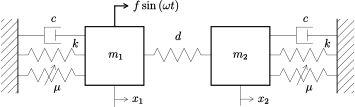
\includegraphics[width=0.5\linewidth]{2dof_duffing/2dof_duffing}
  \caption{Schematic representation of the coupled duffing system}
  \label{fig:duf_schematic}
\end{figure}

For generating data for characterisation with WT and RFS, the system is
simulated using a logarithmic sine sweep with a sweep rate of 1 oct/min.

For identification, a single band-limited (0-15 rad/s) normally distributed
random signal with 5000 points repeated 9 times and a root mean square(rms)
value of 3N is used. This signal is called a multisine. The frequencies are
chosen to include third harmonics of the highest natural frequency.


%%% Local Variables:
%%% mode: latex
%%% TeX-master: "../report"
%%% End:


\chapter{Methods for dection, characterization and estimation}
\label{chap:methods_dec_char_est}

This chapter deals with the identification process as depicted in figure
\ref{fig:ident_process}, and repeated below, treating localised nonlinearities.

\begin{figure}[ht!]
  \centering
  \begin{mdframed}
    \begin{enumerate}
    \item Detection: {\textit Is there?}\\
      Ascertain if nonlinearity exist in the structural behavior, e.g. yes or
      no.
    \item Characterisation: {\textit Where, what and how?}
      \begin{itemize}
      \item Localize the nonlinearity, e.g. at the joint
      \item Determine the type of nonlinearity e.g.  Coulomb friction\\
        More general: is it stiffness or damping nonlinearity or both. In the
        case of stiffness: is it hardening or softening
      \item Select the functional form of the nonlinearity, e.g.
        $f(x,\dot x) = c \sign (\dot y)$
      \end{itemize}
    \item Parameter estimation: {\textit How much?}\\
      Calculate the coefficients of the nonlinearity model, e.g. $c = 5.47$.\\
      (Ideally the uncertainty should be quantified, e.g. in a probabilistic
      sense, $c \sim N(5.47,1)$. But that is a very difficult task and not
      within the scope of this thesis)
    \end{enumerate}
  \end{mdframed}
  \caption{Identification process for nonlinear structural models}
\end{figure}


Methods for detection are only referred, as detection is usual deemed easy
within the framework of localised nonlinearities \autocite{noel2016a}.
Characterisation is done by wavelet transform and restoring force surface, while
estimation is done by FNSI.


%%% Local Variables:
%%% mode: latex
%%% TeX-master: "../report"
%%% End:


\section{Wavelet transform}
\label{sec:wavelet_transform}

Due to the frequency-energy dependence of nonlinear vibrations, giving time
varying frequencies for sine sweeps, the Fourier transform(FT), eq.
\eqref{eq:ft_transform} does not give useful results.
To allow for a varying frequency the Short Time Fourier transform(STFT) can be
used, eq. \eqref{eq:sft_transform}. Here the function to be transformed is
multiplied by a window function $w(t-\tau)$ which is nonzero only for a short
period of time. Practically this correspond to dividing the original signal into
shorter segments of equal length and then calculate the FT of each segments,
giving a 2D representation of the time-varying spectrum.

Often one want a window observation window that changes with frequency. A short
window gives good time resolution, allowing for identification of when frequency
content changes but poor frequency resolution. On the other hand a long window
allows the frequencies to be identified but gives poor time resolution. One such
window that gives a varying length is the Gaussian window function. Used with
STFT, the transfer is called a Morlet wavelet(MW), eq. \eqref{eq:mw_transform}


\begin{align}
  X(\omega) &= \int_{-\infty}^\infty x(t) e^{-i\omega t} \d t
              \label{eq:ft_transform}\\
  X(\omega, \tau) &= \int_{-\infty}^\infty x(t) w(t-\tau)  e^{-i\omega t} \d t
                    \label{eq:sft_transform}\\
  X(a, b) &= \frac{1}{\sqrt{a}} \int_{-\infty}^\infty x(t) \psi\left(\frac{t-b}{a} \right) \d t
            \label{eq:mw_transform}
\end{align}

For the Morlet wavelet the window function is a Gaussian windowed complex
sinusoidal, $\psi(t) = e^{-t^2/2}e^{i\omega t}$. $a$ defines the frequency
resolution by expanding/contracting the window, see figure
\ref{fig:mw_window_length} and, $b$ is the location of the observation window in
the time domain.

\begin{figure}[!ht]
  \centering
  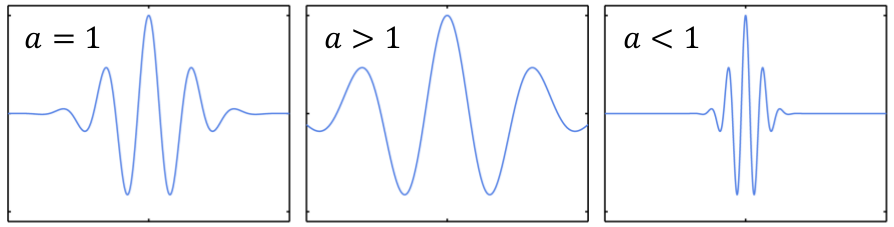
\includegraphics[width=0.8\textwidth]{wt/window_length.png}
  \caption{Influence of $a$ on the window length. Copied from slides given at
    ULG in Liege, Belgium}
  \label{fig:mw_window_length}
\end{figure}


\subsection{Example}
\label{sec:wt_example}

% Figure .. shows a simple example of FT compared to MW for free decay vibrations given by

% \begin{equation}
%   \label{eq:mw_eom}
%   \ddot x + 0.05 \dot x + 0.5 x + x^3 = 0, \quad x_0 = 10, \quad \dot x_0 = 0
% \end{equation}
Figure \ref{fig:mw_2dof}(a) shows the wavelet transform of the coupled duffing
system. Fig \ref{fig:mw_2dof}(b) shows the linear transform for comparison and
fig \ref{fig:mw_2dof}(c) the sweep. For the linear system, the two fundamental
frequencies $\omega_1$ and $\omega_2$ along with the excitation frequency is
clearly seen. Notice that the axis are chosen so the excitation frequency is
seen clearly linear.
For the nonlinear case, higher harmonics, as a multiple of the excitation
frequency, are seen as well. On a magnified plot they are clearly seen to be the
third, fifth and seventh harmonics, with decreasing intensity. This is expected
for a uneven polynomial stiffness and since the third harmonic is present, it
can be concluded that the nonlinear stiffness must be a cubic nonlinearity. Thus
MW can, besides showing that nonlinearity is present, help estimating the type
of nonlinearity. The participation factor of each of the higher harmonics is
computed in section \ref{sec:hb_example}. Fig \ref{fig:mw_2dof}(d) shows the FT
of the linear and nonlinear system. As stated, the FT fails to capture the
changing frequency content of the nonlinear system.

\begin{figure}[!ht]
  \centering
  \begin{subfigure}[b]{0.48\textwidth}
    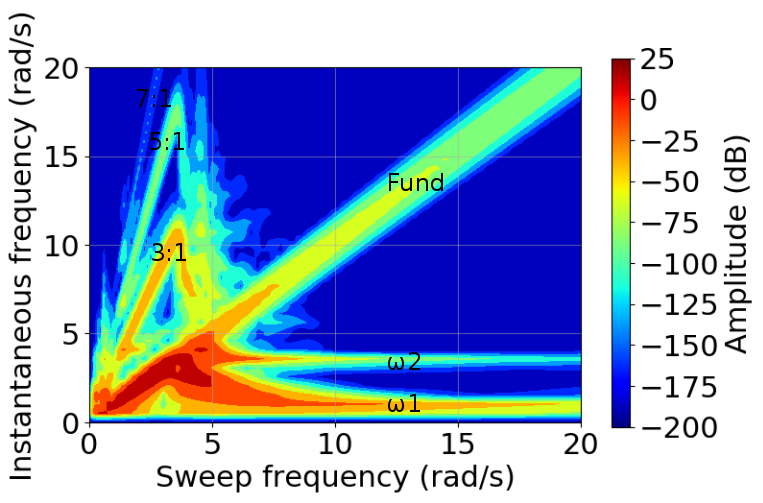
\includegraphics[width=\linewidth]{wt/2dof_wtnlin.png}
    \caption{}
  \end{subfigure}
  ~
  \begin{subfigure}[b]{0.48\textwidth}
    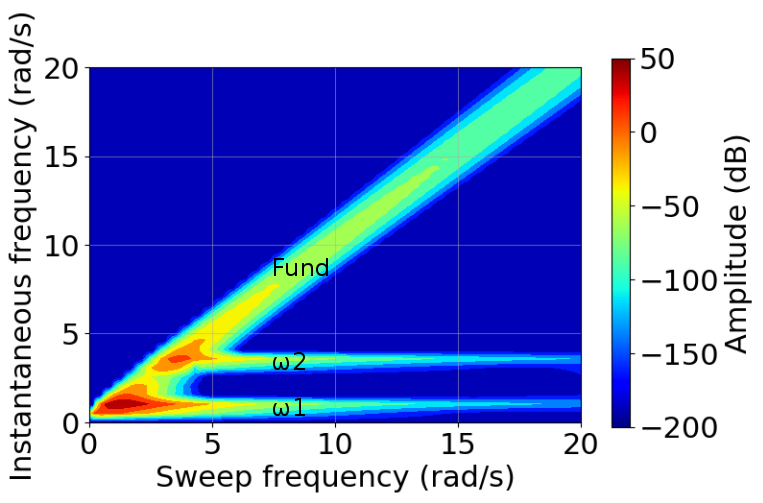
\includegraphics[width=\linewidth]{wt/2dof_wtlin.png}
    \caption{}
  \end{subfigure}
  \\
  \begin{subfigure}[b]{0.49\textwidth}
    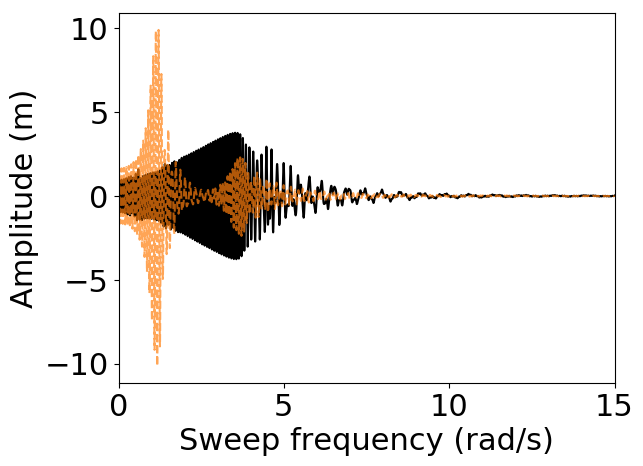
\includegraphics[width=\linewidth]{wt/2dof_wtsweep.png}
    \caption{}
  \end{subfigure}
  \begin{subfigure}[b]{0.49\textwidth}
    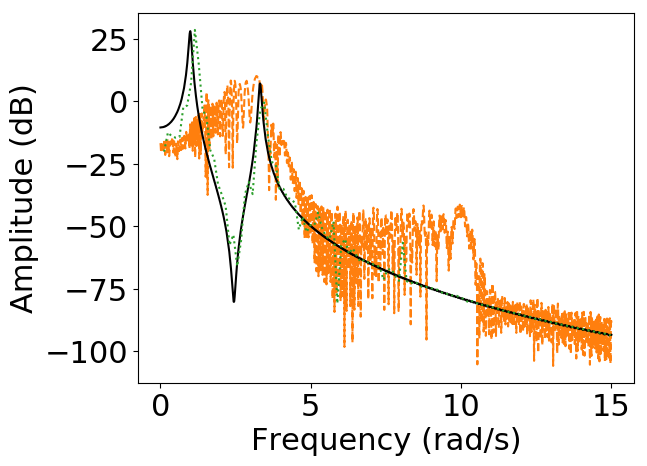
\includegraphics[width=\linewidth, height=5.5cm]{wt/2dof_wtfrf.tikz}
    \caption{}
  \end{subfigure}
  \caption{Morlet wavelet transform of a sine sweep of the coupled duffing
    system. Shown for $x_1$.
    \textbf{(a)}: MW of the nonlinear system;
    \textbf{(b)}: MM of the underlaying linear system;
    \textbf{(c)}: Sine sweep of
    \sampleline{}(nonlinear) and
    \textcolor{orange}{\sampleline{dashed}(linear)} system;
    \textbf{(d)}: Fourier transform of the
    \sampleline{}(nonlinear) and
    \textcolor{orange}{\sampleline{dashed}(linear)} system.
    \textcolor{green}{\sampleline{dotted}(nonlinear multisine)} is the FRF of a
    multisine excitation of the nonlinear system.
  }
  \label{fig:mw_2dof}
\end{figure}


\subsection{Summary}
\label{sec:wt_transform}

The WM shows the instantaneous frequency content of a time signal. Varying
frequency content is a sign of nonlinear vibration and the way the spectra
changes might give clues to the type of nonlinearity.
The frequency spectra is changed in the following way by nonlinear components:

\begin{itemize}
\item \textit{Dissipative NLs} does not affect the resonance frequencies much.
\item \textit{Hardening (softening) elastic NLs} increase (softens) the resonance
  frequencies with amplitude.
\item \textit{Assymmetric elastic NLs} generate even harmonic components.
\item \textit{Symmetric elastic NLs} generate uneven harmonic components.
\item \textit{Nonsmooth elastic NLs} generates wideband frequency components.
\end{itemize}

%%% Local Variables:
%%% mode: latex
%%% TeX-master: "../../report"
%%% End:

\section{Restoring Force Surface}
\label{sec:rfs_description}

The restoring force surface (RFS) method, introduced by \parencite{masri1979a}
and covered in details in \autocite{worden1990a}, have previously been used as a
parameter estimation technique, but is only used as a visual tool for
characterization the functional form of the nonlinearity in this report.

If RFS is used for parameter estimation, an estimation of the inertia for the
system is needed. This either requires an FE model or, for more than a few DOFs,
an complicated algebraic model.

The starting point is Newton's second law of written for a specific DOF located
next to a nonlinear structural component

\begin{equation}
  \label{eq:rfs_newton}
  \sum_{k=1}^{n} m_{i,k} \ddot x_k + f_i(\bm x, \dot{ \bm x}) = p_i
\end{equation}
where $i$ is the DOF of interest, $n$ the number of DOFs in the system, $m_{ik}$
the mass matrix elements, $\bm x$, $\dot{\bm x}$ and $\ddot{ \bm x}$ the
displacement, velocity and acceleration vectors, respectively, $\bm f$ the
restoring force vector encompassing elastic and dissipative effects, and $\bm p$
the external force vector.

Let $j$ denote another measured DOF located across the nonlinear connection, see
figure \ref{fig:rfs_schematic}, a new formulation of \eqref{eq:rfs_newton},
which accounts for the difference in displacement and velocity between the
selected DOFs, is approximated with

\begin{equation}
  \label{eq:rfs_newton2}
  m_{i,i} \ddot x_i +  f_i (x_i - x_j , \dot x_i - \dot x_j) \approx p_i
\end{equation}
where all inertia and restoring force contributions not related to the nonlinear
component are discarded.

\begin{figure}[ht!]
  \centering
  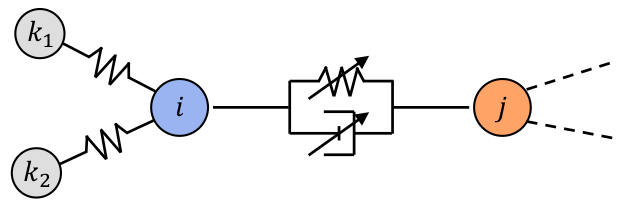
\includegraphics[width=0.5\textwidth]{rfs/rfs_schematic.png}
  \caption{Nonlinear connection between node $i$ and $j$. The linear connections
    $k_{1,2}$ are discarded.}
  \label{fig:rfs_schematic}
\end{figure}

It is further assumed that no external force is applied directly at DOF $i$
(eg. the external force is applied at a different location on the structure), a
rearrangement leads to
\begin{equation}
  \label{eq:rfs}
  f_i (x_i - x_j , \dot x_i - \dot x_j) \approx -m_{i,j} \ddot x_i
\end{equation}

Thus by dropping the constant mass, the nonlinearities can be visualized as the
negative acceleration at one side of the connection, as a function of the
relative displacement and velocity across this connection. From this an adequate
mathematical model can be found.

The shape of $f$ is visualized by plotting the triplet $(x_{i} - x_{j}, \dot
x_{i} - \dot x_{j}, \ddot x_{i})$ The form of elastic (dissipative)
nonlinearities in the connection is visualized by making a slice along the axis
of the zero velocity (displacement) of the restoring force surface plot. Either
prior knowledge about the physics or a least square fit can be used to find the
functional that best represent the nonlinearity.

%The velocity and displacement are found by numerical integration, see section
%\ref{chap:signals}.


The advantages of RFS as presented here, is that it relies exclusively on measured
time series and have a visual understanding. It is not commonly used for
parameter estimation for MDOF systems, due to the need for direct fitting of
Newton's second law.
RFS is also called Accelerated Surface Method (ASM) at times in literature.


The major limitations of the RFS method in general is
\begin{itemize}
\item Requires the nonlinear dynamics to be excited
\item Shows the total restoring force:
  \begin{itemize}
  \item with multiple nonlinearities it is not possible to distinguish them
    uniquely.
  \item If the nonlinear force is of the same magnitude as the linear force, it
    might be necessary to remove a linear trend from the RFS to visualise the
    nonlinear force.
  \end{itemize}
\item Works best swept-sine excitation.
\item Damping characterisation is difficult due to the low numerical magnitude.
\end{itemize}


\subsection{Example}
\label{sec:rfs_example}

Using a sine sweep excitation on the coupled duffing system \eqref{eq:2dof} and
the RFS methodology,
\begin{equation}
  \label{eq:rfs_tol}
  f_i (x_i - x_j , \underbrace{\dot x_i - \dot x_j}_\text{<tol}) \approx - \ddot x_i
\end{equation}
where \textit{tol} determines the slice thickness, the restoring force is
visualised in figs \ref{fig:rfs_full} and \ref{fig:rfs_stiff} for $x_0$ and
$x_1$. A hardening stiffness is seen, without any offset, which correspond to a
uneven nonlinear polynomial stiffness. In this case a third order polynomial for
both DOFs.

\begin{figure}[!ht]
  \centering
  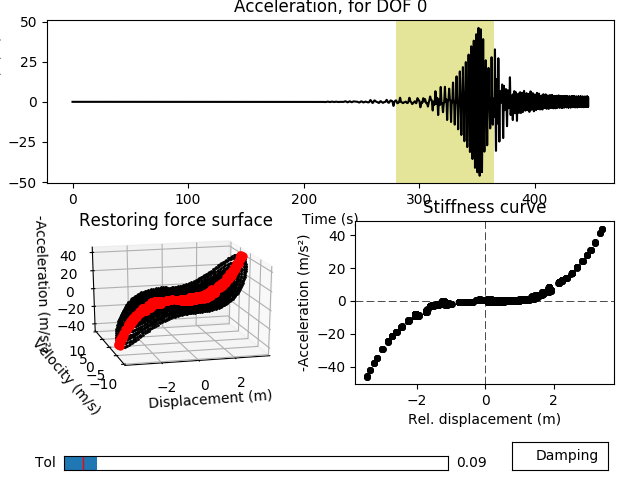
\includegraphics[width=0.8\textwidth]{rfs/sweepvrms3dof0_rfs.png}
  \caption{Interface for selecting the part of the signal used for
    visualising the restoring force of the coupled duffing system
    \eqref{eq:2dof}. Here shown for $x_1$.
    \textbf{upper}: The relevant part of the signal is selected by dragging or
    resizing the yellow rectangle;
    \textbf{left}: Restoring force surface for the selected part of the signal.
    The red line shows the slice;
    \textbf{right}: The visualised stiffness. The slice thickness can be changed
    by dragging the tolerance slider. Damping is visualised by clicking on
    \texttt{damping}.
  }
  \label{fig:rfs_full}
\end{figure}


\begin{figure}[!ht]
  \centering
  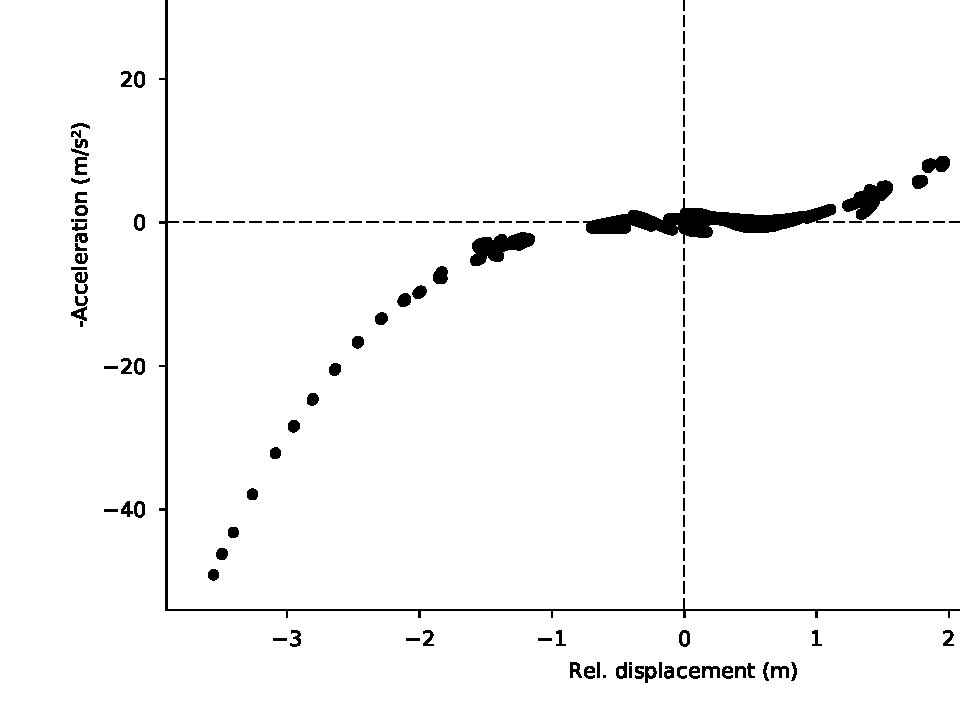
\includegraphics[width=0.6\linewidth, height=6cm]{rfs/sweepvrms3dof1_stiff}
  \caption{The visualised stiffness for $x_2$ from the coupled duffing system
    \eqref{eq:2dof}.
    The figure is extracted from the interface shown in fig. \ref{fig:rfs_full};
    just for $x_2$ instead}
  \label{fig:rfs_stiff}
\end{figure}

\subsection{Summary}
\label{sec:rfs_summary}

The RFS provides a direct visualization of the nonlinear stiffness and, to
lesser extend, damping curve using a SDOF simplification of the EOMs. The steps
are:
\begin{itemize}
\item Instrument the nonlinear connection with two accelerometers and use swept
  sine excitation.
\item Integrate and filter to obtain displacement and velocity.
\item Calculate the 3D acceleration surface over a single connection.
\item Make surface slides to obtain stiffness and damping curve.
\end{itemize}

The success of parameter estimation step is conditional upon an accurate
characterization of all observed nonlinearities.



%%% Local Variables:
%%% mode: latex
%%% TeX-master: "../../report"
%%% End:

 \section{Frequency-domain subspace identification}
\label{sec:freq-doma-subsp}

This section describes a methods for estimation of the underlying linear
frequency response function and nonlinear coefficients for nonlinear systems.
The method is an (nonlinear) extension of linear subspace methods which are able
to deal with multiple-input, multiple-output(MIMO) systems.

The nonlinear subspace methods interpret nonlinearities as unmeasured internal
forces, ie. nonlinearities are seen as cause of distortion on the linear FRF
matrix. Two main nonlinear methods exist, one in time domain: time-domain
subspace identification (TNSI)\autocite{marchesiello2008a} and one in frequency
domain: frequency-domain subspace identification (FNSI)\autocite{noel2013a} .
Both performs equally well in identification and robustness, but the main
benefit of FNSI is that the input time series, when converted to frequency
domain, can be truncated to a frequency interval of interest and thus reduce the
computational time. FNSI is the method used here.



Given the equation of motion for a dynamical system with nonlinearities:

\begin{equation}
  \label{eq:EOM_fnsi}
  \bm M \ddot{\bm q}(t) + \bm C \dot{\bm q}(t) + \bm K \bm q(t) +
  \bm f_{nl} \left( \bm q(t), \dot{ \bm q}(t) \right) = \bm p (t)
\end{equation}

where $\bm M$, $\bm C$ and $\bm K \in \mathbb{R}^{n \times \, n}$ are the
mass, linear viscous damping and linear stiffness matrices; $\bm q(t)$ and
$\bm p(t) \in \mathbb{R}^{n}$ are the generalised displacement and external
force vectors; $\bm f_{nl}(t) \in \mathbb{R}^{n}$ is the essentially nonlinear,
i.e. nonlinearisable, restoring force vector comprising elastic and dissipative
contributions; $n$ is the number of DOFs.


The notation of \eqref{eq:EOM_fnsi} assumes that all linear components of the
restoring forces in the system are included in the matrices $\bm K$ and $\bm
C$. The nonlinear restoring force is expressed by a linear combination of $s$
lumped nonlinearities

\begin{equation}
  \label{eq:nonlin_fnsi_lummped}
  \bm f_{nl} \left( \bm q(t), \dot{\bm q}(t) \right) =
  \sum_{i=1}^s \mu_i \bm b_i \bm g_i \left( \bm q(t), \dot{\bm q}(t) \right)
\end{equation}
where $\mu_i$ is the unknown nonlinear coefficient and $\bm g_i \left( \bm q(t),
  \dot{\bm q}(t) \right)$ is the the corresponding known (identified by eg. RFS)
functional form (or basis function). The location of the nonlinearity is
specified by the boolean vector, $\bm b_i \in \mathbb{R}^{n}$.


Moving the nonlinear terms of \eqref{eq:EOM_fnsi} to the right-hand side

\begin{equation}
  \label{eq:EOM_fnsi_final}
  \bm M \ddot{\bm q}(t) + \bm C_v \dot{\bm q}(t) + \bm K \bm q(t) = -
  \sum_{i=1}^s \mu_i \bm b_i \bm g_i(t) + \bm p(t)
\end{equation}
the system may be viewed as the underlying linear system subjected to the
external force $\bm p(t)$ and the internal feedback force due to nonlinearities,
as shown in figure \ref{fig:fnsi_feedback}.

\begin{figure}[!ht]
  \centering
  % \import{fig/fnsi/}{fnsi_feedback.pdf_tex}
  % 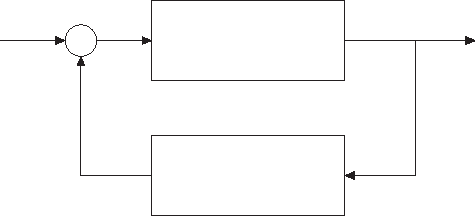
\includegraphics[width=0.5\textwidth]{fnsi/fnsi_feedback}
  \tikzstyle{block} = [draw, fill=white, rectangle, minimum height=3em, minimum width=6em]
  \tikzstyle{sum} = [draw, fill=white, circle, node distance=1.5cm, plus]
  \tikzstyle{input} = [coordinate]
  \tikzstyle{output} = [coordinate]
  \begin{tikzpicture}[auto, node distance=2cm,>=latex']
    \node [input, name=input] {};
    \node [sum, right of=input] (sum) {};
    \node [block, right=1cm of sum, align=left] (system)
      {Underlying linear\\ system: $\bm M, \bm C, \bm K$};
    \node [output, right=2cm of system] (output) {};
    \node [block, below of=system, align=left] (feedback)
      {Nonlinear feedback:\\ $c_a, \bm g_a(\bm y_{nl}(t), \dot{\bm y}_{nl}(t))$};
    \draw [draw,->] (input) -- node {$\bm u(t)$} (sum);
    \draw [->] (sum) -- node {} (system);
    \draw [->] (system) -- node [name=y] {$\bm y, \dot{\bm y}$}(output);
    \draw [-] (y) |- (feedback);
    \draw [->] (feedback) -| node [near end] {} (sum);
  \end{tikzpicture}
  \caption{Feedback interpretation of nonlinear structural dynamics.}
  \label{fig:fnsi_feedback}
\end{figure}


Using the state vector $\bm x = [\bm q, \dot{\bm q}]^T\in\mathbb{R}^r$, the
system \eqref{eq:EOM_fnsi_final} is rewritten as the state space formulation
\begin{equation}
  \label{eq:fnsi_c_state_space}
  \begin{split}
    &\dot{\bm x}(t) = \bm A_c \bm x(t) + \bm B_c \bm e(t) \\
    &\bm y(t) = \bm C \bm x(t) + \bm D \bm e(t)
  \end{split}
\end{equation}
where subscript $c$ denotes {\textit continuous time} and $r=2n$. $\bm e(t) =
\bm p(t)^T, g_1, \dots , g_s]^T \in \mathbb{R}^{n+s}$ is the extended input
vector which concatenates external and nonlinear terms.

State-space and physical matrices have the relations
\begin{equation}
  \label{eq:state_to_physical_mat}
  \begin{split}
  \bm A_c =
  \begin{bmatrix}
    \bm O^{r \times r} & \bm I^{r \times r} \\
    -\bm M^{-1}K     & -\bm M^{-1} \bm C \\
  \end{bmatrix}
  \in \mathbb{R}^{2r \times 2r} , \\
  \bm B_c =
  \begin{bmatrix}
    \bm 0^{r \times 1} & \bm 0^{r \times 1} & ... &
    \bm 0^{r \times 1} & \bm 0^{r \times 1} \\
    -\mu_1 \bm M^{-1} \bm b_1 & -\mu_2 \bm M^{-1} \bm b_2 & ... &
    -\mu_s \bm M^{-1} \bm b_S & -\mu_1 \bm M^{-1} \bm b_1 & \\
  \end{bmatrix}
  \in \mathbb{R}^{(n \times \sigma)} \\
  \bm C =
  \begin{bmatrix}
    \bm I^{n\times n} & \bm I^{n\times n}
  \end{bmatrix}
  \in \mathbb{R}^{(n \times n)} \,\quad
  \bm D = \bm 0^{n\times\sigma}
\end{split}
\end{equation}
The state matrices are: $\bm A$ and $\bm B$ the input and nonlinear coefficients
matrix, the output matrix $\bm C$ and the direct feed through matrix $\bm D$.

This way of characterizing the system above is the same as with TNSI. Using a
Fourier transform, the system is

\begin{equation}
  \label{eq:fnsi_freq_state}
  \begin{aligned}
    z_k \bm X &= \bm A_d \bm X(k) + \bm B_d \bm E(k) \\
    \bm Y(k) &= \bm C \bm X(k) + \bm D \bm E(k)
\end{aligned}
\end{equation}
where $z_k = e^{(2i\pi k/N_s)}$ is the Z-transform variable for discrete time
models and $N_s$ the number of recorded samples in the time series. $\bm X, \bm
Y$ and $\bm E$ are the discrete Fourier transforms of $\bm x, \bm y$ and $\bm e$.

\textbf{Noget om at fitte en discrete time model til continuous time for sikre
  good conditioning}

\subsection{The output-state-input equation}

The extended input $\bm E$ and output $\bm Y$ is known. The system matrices $\bm
A_d, \bm B_d, \bm C$ and $\bm D$ needs to be determined along with the system
order $r$. Frequency-domain subspace methods estimates these matrices based on a
reformulation of the state-space eqs. \eqref{eq:fnsi_freq_state} in matrix form.
The matrix of the measured output spectra is

\begin{equation}
  \bm Y_i =
  \begin{bmatrix}
    \bm Y(1) & \bm Y(2) & \dots & \bm Y(N) \\
    z_1\bm Y(1) & z_2\bm Y(2) & \dots & z_F\bm Y(N) \\
    z^2_1\bm Y(1) & z^2_2\bm Y(2) & \dots & z^2_F\bm Y(N) \\
    \vdots \\
    z^{i-1}_1\bm Y(1) & z^{i-1}_2\bm Y(2) & \dots & z^{i-1}_F\bm Y(N)
  \end{bmatrix}
\end{equation}
which by defining $\xi = \text{diag}(z_1, z_2, \dots, z_N)$ is recast to

\begin{equation}
  \begin{aligned}
    \bm Y_i =
    \begin{bmatrix}
      \bm Y^T & (\bm Y \xi)^T & \dots & (\bm Y \xi^{i-1})^T
    \end{bmatrix}^T \\
    \bm E_i =
    \begin{bmatrix}
      \bm E^T & (\bm E \xi)^T & \dots & (\bm E \xi^{i-1})^T
    \end{bmatrix}^T
  \end{aligned}
\end{equation}
where $i$ is the user-defined number of block rows in $\bm Y_i$ and $N$ the
number of frequency lines used for identification.

Introducing the extended observability matrix
\begin{equation}
  \bm \Gamma_i =
  \begin{bmatrix}
    \bm C^T & (\bm C \bm A)^T & \dots & (\bm C \bm A^{i-1})^T
  \end{bmatrix}^T
\end{equation}
and the lower-block triangular Toeplitz matrix

\begin{equation}
  \bm H_i =
  \begin{bmatrix}
    \bm D                   & \bm 0                   & \bm 0                   & \dots & \bm 0 \\
    \bm C \bm B             & \bm D                   & \bm 0                   & \dots & \bm 0 \\
    \bm C \bm A \bm B       & \bm C \bm B             & \bm D                   & \dots & \bm 0 \\
    \vdots \\
    \bm C \bm A^{i-2} \bm B & \bm C \bm A^{i-3} \bm B & \bm C \bm A^{i-3} \bm B & \dots & \bm D
  \end{bmatrix}^T
\end{equation}

By recursive use of eq. \eqref{eq:fnsi_freq_state} \autocite{noel2013a}, the
output-state-input matrix equation, which is used for estimation in the subspace
method, is obtained
\begin{equation}
  \label{eq:fnsi_state_matrix}
  \bm Y_i = \bm \Gamma_i \bm X + \bm H_i \bm E_i
\end{equation}


\subsection{Estimation of state matrices}

The subspace method is applied to eq. \eqref{eq:fnsi_state_matrix} in order to
estimate $\bm \Gamma_i$ and the system order $n_s$. When $\bm \Gamma_i$ is
estimated, the state matrices of eq. \eqref{eq:fnsi_freq_state} are extracted
and calculated.

The method have two main steps:
\begin{itemize}
\item Eliminate the term depending on nonlinearities and forces in eq.
  \eqref{eq:fnsi_state_matrix}. This is done by projecting the equation onto the
  orthogonal complement of $\bm E_i$,
  \begin{equation}
    \bm Y_i / \bm E_i^\perp = \bm \Gamma_i \bm X / \bm E_i^\perp = \mathcal{P}
  \end{equation}
  The geometrical interpretation of this is shown in figure
  \ref{fig:fnsi_geometric} for the 2d case.

  $\Gamma_i$ is then estimated from a singular value decomposition(SVD) of the
  projection $\mathcal{P}$
\item When $\Gamma_i$ is estimated, the four state space matrices ($\bm A, \bm
  B, \bm C, \bm D$) are calculated. See figure \ref{fig:fnsi_methodolgoy} for a
  overview and \autocite{noel2013a} for more details.
\end{itemize}

\begin{figure}[!ht]
  \centering
    %\def\svgwidth{3cm}
  \import{fig/fnsi/}{fnsi_geometric2.pdf_tex}
  \caption{Geometric interpretation of eq. \eqref{eq:fnsi_state_matrix} in two
    dimensional space. The orthogonal complement of $\bm E_i$, $\bm E_i^\perp$,
    is the set of all vectors that are orthogonal to every vector of $\bm E_i$
    (thus it is also the null space of $\bm E_i$).
    In the 2d case, $\bm E_i^\perp$ is simply the vector perpendicular to $\bm
    E_i$, and the projection of $\bm Y_i$ cancels the extended input term $\bm
    H_i \bm E_i$. In 3d the orthogonal complement of the plane spanned of two
    vectors $\bm u$ and $\bm v$, is the subspace formed by all normal vectors to
    that plane.
  }
  \label{fig:fnsi_geometric}
\end{figure}


\begin{figure}[!ht]
  \centering
  \begin{mdframed}
    \begin{enumerate}
    \item Choose the index $i$ and the number of processed frequency lines N
    \item Concatenate external forces and nonlinearities to form the extended
      input spectra $E_i$
    \item Compute the orthogonal projection
      \begin{equation*}
        \mathcal{P} = \bm Y_i / \bm E_i^\perp
      \end{equation*}
      using QR-decomposition.
    \item Compute the SVD of $\mathcal{P}$
      \begin{equation}
        \label{eq:fnsi_svd}
        \mathcal{P} = \bm U \bm S \bm V
      \end{equation}
    \item Determine model order $n_s$ from singular values in $\bm S$ or from a
      stabilisation diagram. Truncate $\bm U$ and $\bm S$ accordingly to define
      $\bm U_1$ and $\bm S_1$.
    \item Estimate the extended observability matrix $\bm \Gamma_i$
      \begin{equation*}
        \hat{\bm \Gamma}_i = \bm U_1 \bm S_1^{1/2}
      \end{equation*}
    \item Estimate $\bm A$ using the shift property of $\bm \Gamma_i$,
      \begin{equation*}
        \underline{\bm \Gamma_i} \hat {\bm A} = \overline{\bm \Gamma_i}
        \iff
        \hat {\bm A} = \underline{\bm \Gamma^+_i} \overline{\bm \Gamma_i}
      \end{equation*}
      where $\underline{\bm \Gamma_i}$ and $\overline{\bm \Gamma_i}$ are the
      matrix $\bm \Gamma_i$ without its first and last $l$ rows.
      $\bm C$ is extracted as the first block row of $\bm \Gamma_i$.
    \item Estimate $\bm B$ and $\bm D$ by defining the transfer function matrix
      $\bm G_s$,
      \begin{equation*}
        \bm G_s(k) = \bm C(z_k \bm I - \bm A)^{-1} \bm B + \bm D
      \end{equation*}
      and minimise the difference between the measured and modelled output
      spectra in a linear least square sense, i.e.
      \begin{equation*}
        \hat {\bm B}, \hat {\bm D} = \arg \min_{\bm B, \bm D} \sum_{k=1}^F |\bm Y(k) - \bm G_s(k) \bm E(k)|^2
      \end{equation*}
    \item Convert $\bm A, \bm B, \bm C$ and $\bm D$ into continuous-time
      matrices and form the extended FRF $\bm H^e(\omega)$.
      \begin{equation}
        \label{eq:extend_FRF_He}
        \bm H^e(\omega) = \bm C_c \left(j \omega \bm I^{n \times n} - \bm A_c \right)^{-1} \bm B_c^e + \bm D_c^e
        \in \mathbb{C}^{(l \times \sigma)}
      \end{equation}
    \item Estimate the nonlinear coefficients $\mu_j$ and the linear FRF matrix
      $\bm H(\omega)$.
      The FRF matrix of the underlying linear system $\bm H(\omega) \in \mathbb{C}^{(l
        \times l)}$ and the nonlinear coefficients $\mu_s$ are found from
      \eqref{eq:extend_FRF_He} as
      \begin{equation}
        \label{eq:FRE_H}
        \bm Q(\omega) = \bm H(\omega)
        \begin{Bmatrix}
          \bm I^{l\times 1} & -\mu_1\bm b_1 & ... & -\mu_s \bm b_s
        \end{Bmatrix}
        \bm E (\omega)
        =
        \bm H^e(\omega) \bm E(\omega)
      \end{equation}
    \end{enumerate}
  \end{mdframed}
  \caption{Overview of the FNSI methodology}
  \label{fig:fnsi_methodolgoy}
\end{figure}



Three assumptions are assumed to be fulfilled for the subspace methods,
\begin{enumerate}
\item All the linear modes of vibration in the frequency band of interest are
  excited or, alternatively, they are all observable in input-output data.
\item The row space of the states $\bm X$ and of the extended input spectra
  matrix $\bm Y_i$ does not share information,
  \begin{equation*}
    \text{span}_{\text{row}} (\bm X) \cap \text{span}_{\text{row}}(\bm E_i) = 0
  \end{equation*}
\item The extended inputs $\bm E_i$ are of full rank, i.e.,
  \begin{equation*}
    \text{rank}(\bm E_i) = \sigma i
  \end{equation*}
  Excitations and the nonlinearities have to be such that the inversion of the
  problem is well-posed
\end{enumerate}

To expand on the second assumption:
The state term $\bm A \bm X$ contains linear stiffness and damping information.
If constant and/or linear terms are introduced in the nonlinear basis functions,
the intersection between the states and the extended inputs $\bm E_i$ is no
longer empty, which violate the assumption.
This requires nonlinear basis functions to be nonlinearisable, i.e. they should
be zero and have zero slope at the origin.



{\textbf Dimension:}

$\bm b_s \in \mathbb{R}^l$ is a boolean vector specifying the location of the
nonlinearity $\mu_s$.
$\sigma = m + s$, where $s$ is the number of lumped nonlinearities and $m \leq
r$ is the number of {\textit measured applied forces}. $l \leq r$ is the number of
{\textit measured applied displacement}.
$n$ is the model order, not $n=2r$ as used in the beginning of the article, and
$r$ is number of DOFs.



\subsection{Types of nonlinear functional}
\label{sec:fnsi_functional}


As stated, the nonlinear basis functions should be zero and have zero slope at
the origin. For continuous nonlinear restoring force, polynomial functions with
order chosen from RFS-plots can be used. For discontinuous systems, e.g. contact
polynomials might not be well suited, for instance higher order polynomials
exhibit oscillations around the origin. An alternative is to use piecewise cubic
spines instead. Even if they cannot realise a perfect fitting (they are
continuous by nature), they are appropriate for representing sudden events,
like sharp changes in stiffness/damping curves.

In order to get the basis functions from cubic splines, the abscissas of knots
is specified on beforehand and the ordinate as free parameters. FNSI then
estimate the ordinate.
Choosing the number of knots and their abscissas should rigorously be sought by
minimising the difference in some metric between the predictions of the
non-linear model and measured data. In reality it is still done by trial and
error.

Using cubic splines might be termed \textit{gray box} identification where using
polynomials is \textit{white box}. The difference is that with gray box, the
nonlinearities are described by functionals that may represent a vast variaty of
nonlinear behaviour and thus requiring less specific knowledge of the underlying
physics.


\subsection{Estimating model order}

In the presence of non-linearities, the model order translates the number of
underlying linear modes excited in the output data. This implies that, similarly
to linear system identification, a stabilisation analysis can be utilised as
decision-making tool instead of looking at the singular values of $\bm S$,
\eqref{eq:fnsi_svd}. The stabilisation diagram shows the stabilisation of the
estimated linear parameters: stabilisation in frequency, stabilisation in
damping and stabilisation of the mode. If all three parameters are stabilised
the mode is full stabilised. Stabilisation is compared to the same mode for one
model order higher. Stabilisation for the mode is calculated by the modal
assurance criterion(MAC) \autocite{Allemang2003},

\begin{equation}
  MACX(r,q) = \frac{|\bm \psi^T_r \bm \psi^*_q|^2}
  {\left( \bm \psi^T_r \bm \psi^*_r \right)\left( \bm \psi^T_q \bm \psi^*_q \right)}
\end{equation}

% For simulated data without noise, tolerances for frequency, damping and mode
% stabilisation are $0.5\%, 2\%, 0.98$ respectively.


If the model order is chosen too low, it will result in unmodelled dynamics,
whereas too large orders lead to overmodelling issues such as an increase of the
noise sensitivity of the model. It should be noted that model selection requires
that adequate basic functions are used.

Without anticipating the example, a stabilisation diagram for the coupled
duffing system is shown in figure \ref{fig:fnsi_stab} along with singular values
of $\bm S$ in figure \ref{fig:fnsi_svg}. The two modes are clearly seen.
From the stabilisation diagram a model order of four is chosen. This gives
stabilisation in the linear parameters. The plot of the singular values shows a
jump of six orders magnitude between model order four and five, verifying the
chosen model order.
In general only the stabilisation diagram is used; the singular value plot is
only used if a stabilisation diagram is not implemented.

\begin{figure}
  \centering
  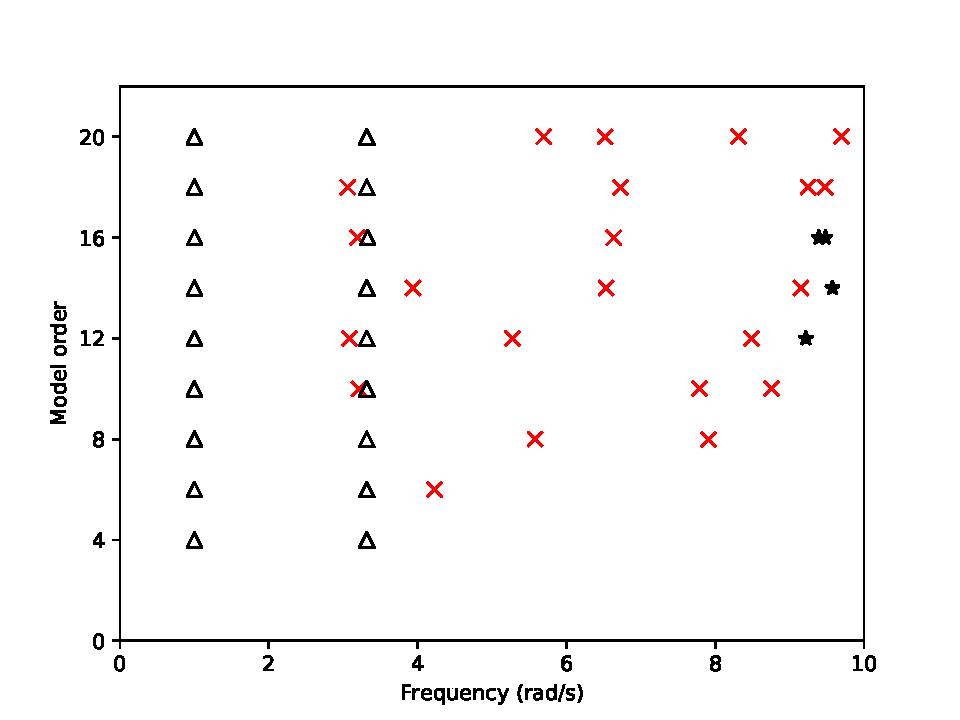
\includegraphics[width=0.8\linewidth]{fnsi/vrms3_stab.tikz}
  \caption{Estimation of model order. Stabilisation diagram with linear FRF overlayed.
    $\pmb\times$(red): new pole;
    $\pmb\star$: stabilisation in natural frequency;
    $\pmb\square$: extra stabilisation in damping ratio;
    $\pmb\circ$: extra stabilisation in MACX;
    $\pmb\triangle$: full stabilisation.
    Stabilisation thresholds in natural frequency, damping ratio and MACX value
    are $0.5\%, 2\%, 0.98$, respectively. Not all types of stabilisation are
    present here.
  }
  \label{fig:fnsi_stab}
\end{figure}

\begin{figure}
  \centering
  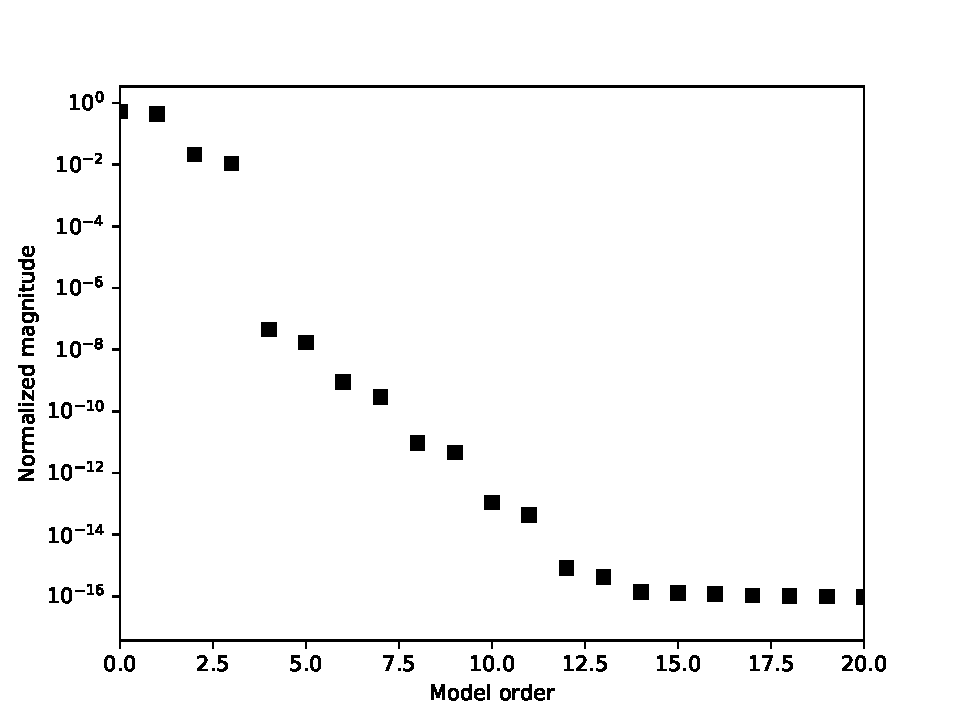
\includegraphics[width=0.6\linewidth, height=6cm]{fnsi/vrms3_svg.tikz}
  \caption{First tventy singular values. A jump of six orders magnitude is seen
    between model order four and five.}
  \label{fig:fnsi_svg}
\end{figure}

The determination of the model order is very simple and clear here. For larger system this
might not be the case, as seen with the more involved examples in section
\ref{cha:application}.

\subsection{Example}
\label{sec:fnsi_example}


Figure \ref{fig:periodicity} shows the periodicity of the recorded signal. The
signal of the last recorded period is compared to previous periods. For
identification, multiple periods can be used but transient effects should not be
present; which is indicated by a low periodicity.

\begin{figure}[!ht]
  \centering
  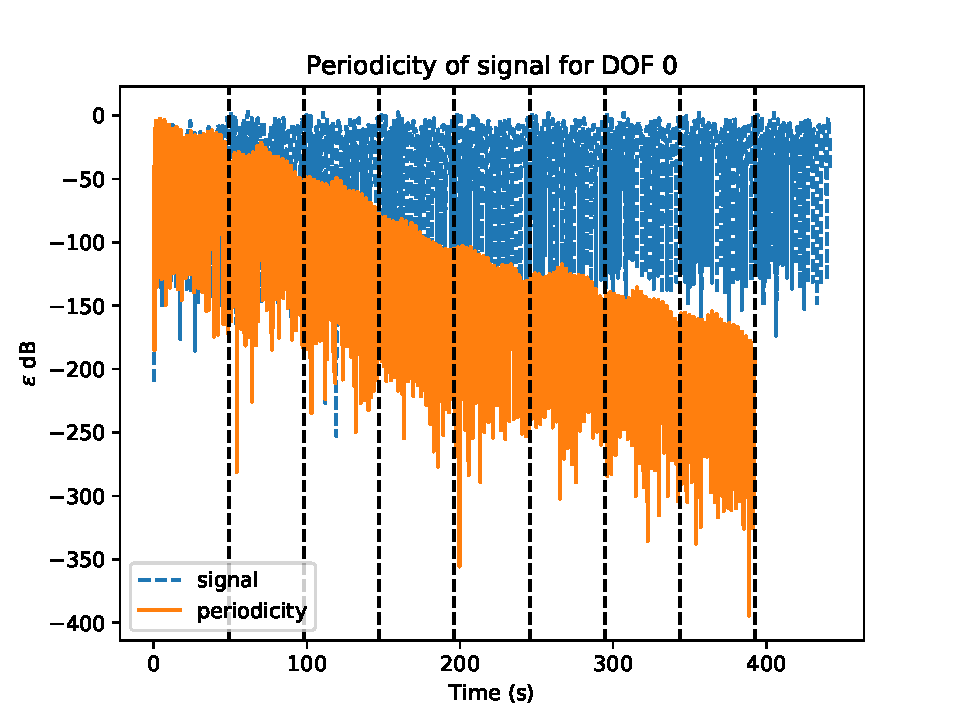
\includegraphics[width=0.7\linewidth]{signal/frf_per}
  \caption{Periodicity of recorded signal at DOF 0. Vertical lines indicate
    periods. A low periodicity shows that transient effects have died out}
  \label{fig:periodicity}
\end{figure}


The estimation of the nonlinear parameters of the coupled duffing system is
shown in figure \ref{fig:fnsi_knl} for model order four. The variation of the
real part of$\mu$ is shown in a 1\% interval, with very little frequency
dependency in the frequency range of interest. The imaginary part is about three
orders of magnitude smaller. Both indicates a good quality of the estimation.
The spectral averages are
\begin{equation}
  \begin{aligned}
    \Re (\mu_1) = 1.000, \quad \Im (\mu_1) = 1.09 \times 10^{-4} \\
    \Re (\mu_2) = 1.000, \quad \Im (\mu_1) = 7.73 \times 10^{-4}
  \end{aligned}
\end{equation}
matching the simulated values well.

\begin{figure}[!ht]
  \centering
  \begin{subfigure}[b]{0.45\textwidth}
    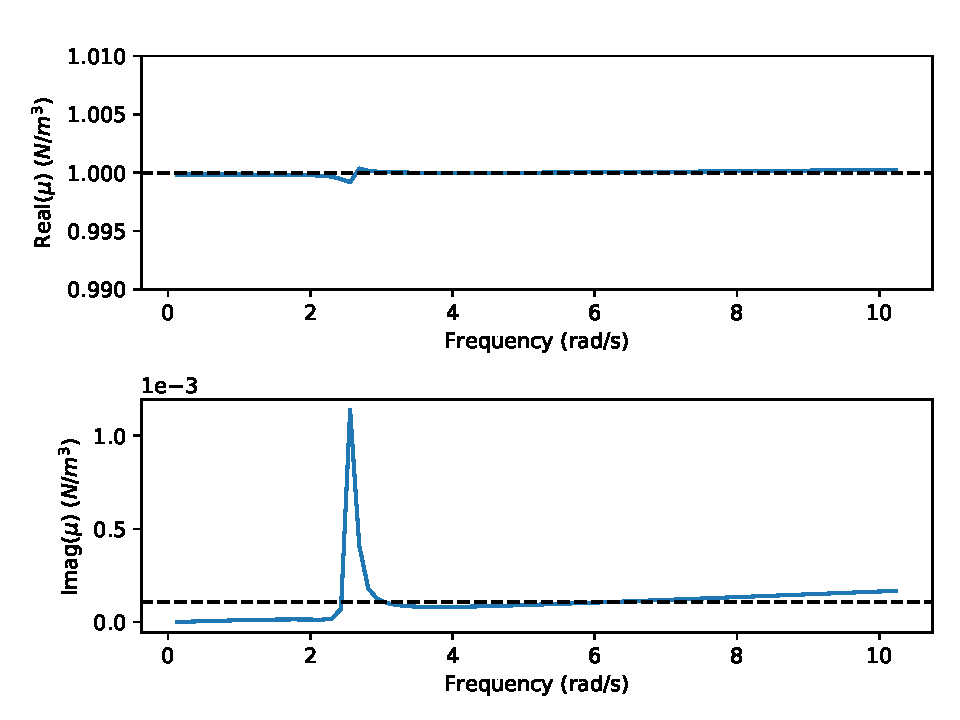
\includegraphics[width=\linewidth]{fnsi/vrms3_knl0.tikz}
    \caption{}
  \end{subfigure}
  ~
  \begin{subfigure}[b]{0.45\textwidth}
    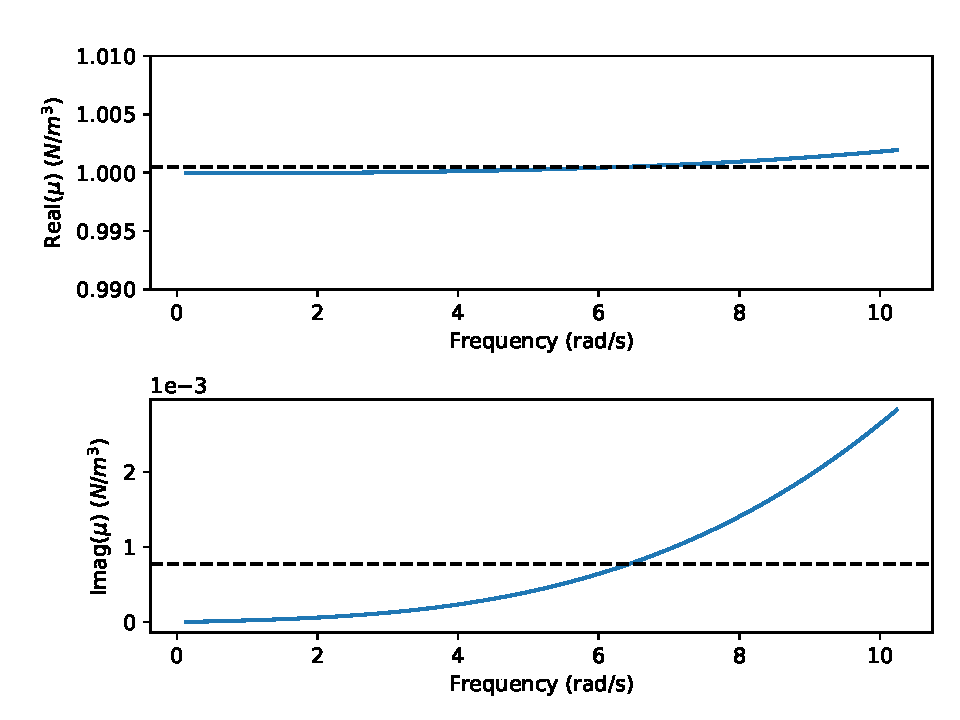
\includegraphics[width=\linewidth]{fnsi/vrms3_knl1.tikz}
    \caption{}
  \end{subfigure}
  \caption{Real and imaginary part of estimated nonlinear coefficients $\mu_1$
    and $\mu_2$. The variation of Re($\mu$) is shown in a 1\% interval, with
    very little frequency dependency in the frequency range of interest.
    The imaginary part is about three orders of magnitude smaller. Both
    indicates a good quality of the estimation.
    \textbf{(a)}: $\mu_1$;
    \textbf{(b)}: $\mu_2$.
  }
  \label{fig:fnsi_knl}
\end{figure}

The FNSI method also estimate the underlaying linear properties. As seen from
table \ref{tab:fnsi_eigen}, the linear parameters are identified correctly.
Ensuring that linear parameters are identified, also shows that nonlinear
coefficients are identified correct.

\begin{center}
  \begin{tabular}{*{3}{c}}
    \hline
    Mode & Frequency (rad/s) & Damping ration (\%) \\
    1 & 1.00 & 5.00 \\
    2 & 3.32 & 1.51 \\
    \hline
    1 & 1.19 & 3.96 \\
    2 & 3.40 & 1.41 \\
    \hline
  \end{tabular}
  \captionof{table}{Estimated linear natural frequencies and damping ratios for
    the coupled Duffing system.
    \textbf{(upper)}: Nonlinear identification with FNSI;
    \textbf{(lower)}: Linear identification
  }
  \label{tab:fnsi_eigen}
\end{center}

Figure \ref{fig:fnsi_H1} shows the transfer function. The linear transfer
function found by FNSI match the theoretical linear transfer function.

\begin{figure}[!ht]
  \centering
  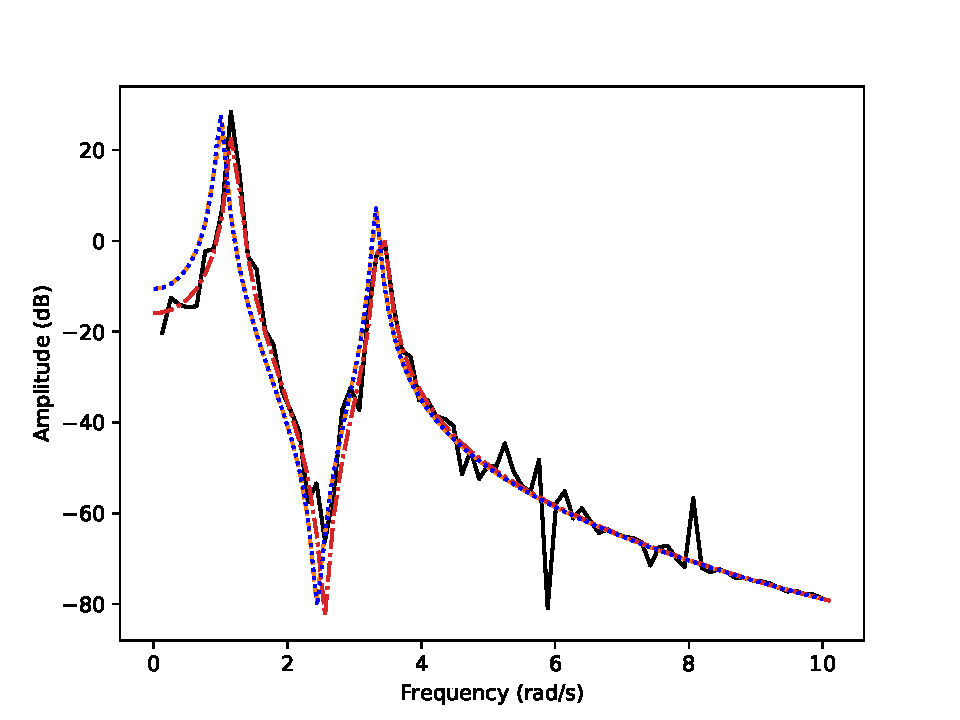
\includegraphics[width=0.8\linewidth]{fnsi/vrms3_H1.tikz}
  \caption{Transfer function $H_1$ for the coupled duffing system.
    \sampleline{}(black): H1 from signal;
    \sampleline{dash pattern=on .7em off .2em on .2em off .2em}\textcolor{red}{(red)}: Linear identified;
    \sampleline{dashed}\textcolor{orange}{(orange)}: Linear identified from FNSI;
    \sampleline{dotted}\textcolor{blue}{(blue)}: Theoretical linear
    % \sampleline{dash pattern=on .7em off .2em on .05em off .2em}
  }
  \label{fig:fnsi_H1}
\end{figure}

\subsection{Estimation error}
\label{sec:fnsi-estimation-error}

It seems that the FNSI method works quite well - both nonlinear and linear
parameters are estimated with high accuracy - and indeed it does work well. But
it is not exact, as will be shown here: the method introduce spurious undesired
terms, and even if they are small in magnitude, they still alters the
identified model.



\subsection{Summary}
\label{sec:summary-fnsi}

The FNSI method is able to identifying multiple nonlinear parameters for system
with many DOFs. It differs from time domain methods, with the ability to
truncate measured signals to the frequency intervals of interest making
computations faster for large systems.

Characterisation of the nonlinearity is important to get a good identification.
If there is limited knowledge about the nonlinearity, cubic splines can be used
instead of polynomials.
In general the following steps can be used to check the validity of the
identification:

\begin{itemize}
\item Check the stabilisation of the first mode.
\item Check the modal parameters compared to linear identification.
\item Check the stability of the nonlinear coefficients versus frequency.
\item Check the magnitude of the imaginary parts of the coefficients.
\end{itemize}


% \begin{table}[h]
% % scale down the table to the textwidth
% \resizebox{\textwidth}{!}{
% %  \begin{tabularx}{\textwidth}{XXX}
%   \begin{tabular}{lll}
%     \hline
%     Property              & TNSI & FNSI \\
%     \hline
%     Domain & Time & Frequency \\
%     MIMO  & Yes & Yes \\
%     Iterative & No & No \\
%     Data exploited & Transient & Steady State \\
%     Data pre-processing & No & DFT \\
%     Frequency-domain data reduction & Not possible & User-selected bands \\
%     Characterization capability & Multiple-term model and {\textit a posteriori}
%                                   discrimination & Identification error criterion\\
%     Stabilization diagram &  Yes & Yes \\
%     Accuracy of the linear parameter estimates   & High, with larger errors on
%                                                    damping ratios & High, with larger
%                                                                     noise variability\\
%     Accuracy of the nonlinear parameter estimates & High, with larger noise variability & High, with larger
%                                                                                           frequency dependence\\
%     Computational burden & Moderate & Low\\
%     \hline
%   \end{tabular}}
%   \caption{Summary of the properties and identification capabilities of the TNSI
%     and FNSI methods, \citet{noel2014a}}
%   \label{tab:tnsi_fnsi_comparison}
% \end{table}


% Question.
% Dear Jean-Philippe,

% I was at your Nolinsys course in september and would like to demonstrate to my
% supervisor, Jon Juel Thomsen, DTU, how you do parameter estimation.
% So following your paper:
%     Method by J.P Noel. Described in article
%     "Frequency-domain subspace identification for nonlinear mechanical systems"
%     http://dx.doi.org/10.1016/j.ymssp.2013.06.034

% I have done steps up till 10, ie. I can estimate/calculate \hat{E, B, C ,D}
% in step 9 but then I don't know what to do about equation (45).
% I have copied t equations, with dimensions, from your article. See the attached pdf.

% So my question is:
% How do I extract H and \mu from eq. 1.2 (45)? I have calculated H^e, but do not
% understand how to proceed.

% Here is a snippet from my code:

% # step 10
% (loop over omegas: I know it is a bit inefficient, this is just to understand your paper.)
% omegas = range(0,100) # just some range of interest
% for idx, omega in enumerate(omegas):
%     He = C.dot(linalg.inv(np.eye(n,dtype=complex)*1j*omega - A).dot(B)) + D
%     # Calculate H, extract mu's and save in matrix
%     H = ?
%     mu[:,idx] = 



% JUST a note:
% I have also looked at your ph.d thesis. There the formulation seems a bit
% different than in the article, ie:
% Q = H [I^(n,n)  -mu_1 * I^(n,n)  ...  -mu_s * I^(n,n)] E = H^e E

% ie. H is just extracted as the first n columns, as you also write.



%%% Local Variables:
%%% mode: latex
%%% TeX-master: "../../report"
%%% End:



\chapter{From identification to design}
\label{chap:ident_to_design}

This chapter deals with the prediction of behaviour of nonlinear system, after
nonlinear components have been determined. Paraphrased it could be called
\textit{virtual prototyping}. Here methods to detect bifurcations, stability and
internal resonance are presented. The long-term ambition is to use this
knowledge to understand and improve design, taking nonlinear behaviour into
account.


This chapter represent a change of methodology. Where the methods for
identification in the previous chapter relied exclusively on time signals, the
methods of this chapter relies exclusively on FE models.
The information from identification is used to build
an accurate computer model.

Two methods are treated: Harmonic balance(HB) continuation, used for computation
of NFRC and detecting and identifying bifurcations, and nonlinear normal
modes(NNM) continuation, used to detect internal resonance.

Before presenting the methods, the concept of NNMs is reviewed.



% Måske til opsummering:
% (This is a step forward from the traditional methods used today where designs are
% based on shaping resonance(by solving eigenvalue problems) and validated with
% modal responses from experimental data.)


%%% Local Variables:
%%% mode: latex
%%% TeX-master: "../report"
%%% End:



\section{Periodic solution}
\label{sec:periodic-solution}

Before turning to the methods themselves, a few concepts will be revisited.
Computing the periodic solution of a nonlinear system means searching for a
solution $\bm x$ to

\begin{equation}
    \label{eq:per_eom}
  \bm M \ddot{\bm x}(t) + \bm C \dot{\bm x}(t) + \bm K \bm x(t) +
  \bm f_{nl} \left( \bm x(t), \dot{ \bm x}(t) \right) = \bm p (t)
\end{equation}
that satisfies a periodicity condition
\begin{equation}
  \label{eq:per_condtion}
  \bm x(t+T) = \bm x(t)
\end{equation}
where $T$ is the period. This is a boundary value problem(BVP). By periodic
solution, steady state conditions are implied. Stability of the periodic
solution will also be addressed.


There are at least three ways to describe such a periodic solution.

\begin{itemize}
\item Provide initial condition $\left[\bm x_0, \dot{\bm x}_0 \right]$ and the
  period $T$. Then do time integration over $T$.
\item Use Fourier series and the period $T$
\item Use piecewise polynomial functions and the period $T$
\end{itemize}

In this section methods for finding the first and second representations of a
periodic solution is described. They are denoted the shooting method and
harmonic balance method respectively. The one not covered is called
Orthogonal collocation. The shooting method is used as part of calculating NNMs
and harmonic balance is used for bifurcation analysis. Both methods could be
used for either tasks, but as both are popular it is instructive to present
both.

\subsection{Shooting method}
\label{sec:shooting_method}

With the shooting method one finds, in an iterative way, the initial state $\bm
z = [\bm x, \dot{\bm x}]^T$ and period $T$ that describes a periodic
motion \autocite{nayfeh2008applied}.

One start by guessing on a periodic steady state(ie. initial state
and period) and then \textit{shoots} forward one period with the hope of
arriving close to the guessed initial state. The difference between the initial
and final states is used to correct the initial state, and the method
\textit{shoots} forward another period and continue until final and initial
state match.
The final state is found by time integration, see appendix
\ref{chap:newmark-integration} for details on the nonlinear Newmark integration.
The corrections are done by Newton-Rahpson iterations.

The eom \eqref{eq:per_eom} is recast into state space form. Since this method is
used for NNMs, they are recast in undamped and unforced form, ie. the underlaying
hamiltonian structure.

\begin{equation}
  \label{eq:sm_state}
  \dot{\bm z} = \bm h_{ham} (\bm z) =
  \begin{bmatrix}
    \dot{\bm x} \\
    -\bm M^{-1}(\bm K \bm x  + \bm f_{nl})
  \end{bmatrix}
\end{equation}


A solution $\bm z_p(t, \bm z_0)$ is a periodic solution of the autonomous system
eq. \eqref{eq:sm_state} if $\bm z_p(t, \bm z_{0}) = \bm z_p(t+T, \bm z_{0})$
where $T$ is the minimal period. Unlike forced motion, the period is not known a
priori. The notation is written as $\bm z(t)=\bm z(t, \bm z_0)$ to indicate the
dependence on initial conditions $\bm z(0, \bm z_0) = \bm z_0$.
From above, the periodic condition is

\begin{equation}
  \label{eq:sm_per_cond}
  \bm h(\bm z_{p0},T) \equiv \bm z(T, \bm z_{p0}) - \bm z_{p0} = \bm 0
\end{equation}
where $\bm h$ is called the shooting function.


To make the solution $\bm z(t)$ uniquely defined, the phase must be fixed. If
$\bm z(t)$ is a solution to \eqref{eq:sm_state} then $z(t + \Delta t)$ is
geometrically the same solution in state space for any $\Delta t$. Ie. the
initial condition $\bm z_{0}$ can be arbitrarily chosen anywhere on the
periodic solution. To prevent this, a phase condition $g(\bm z_{0})=0$ is set
as a additional condition. Most phase conditions imposes one of the unknowns to
be set to 0, e.g. the initial displacement or velocity of a DOF(often velocity).
See figure \ref{fig:sm_phase} for a illustration of different phases for the
periodic solution.

\begin{figure}[!ht]
  \centering
  \begin{subfigure}[b]{0.45\textwidth}
    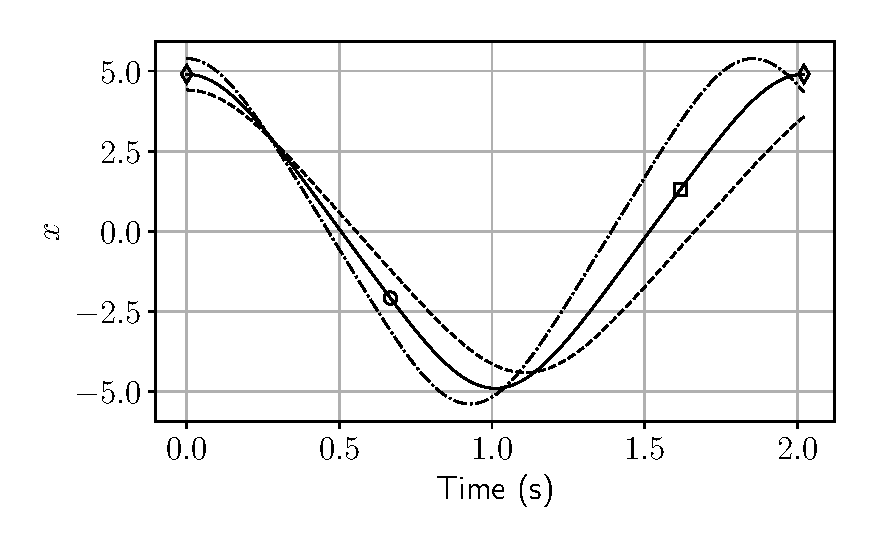
\includegraphics[width=\textwidth, height=5cm]{nnm/duff_per_time}
  \end{subfigure}
  ~
  \begin{subfigure}[b]{0.45\textwidth}
    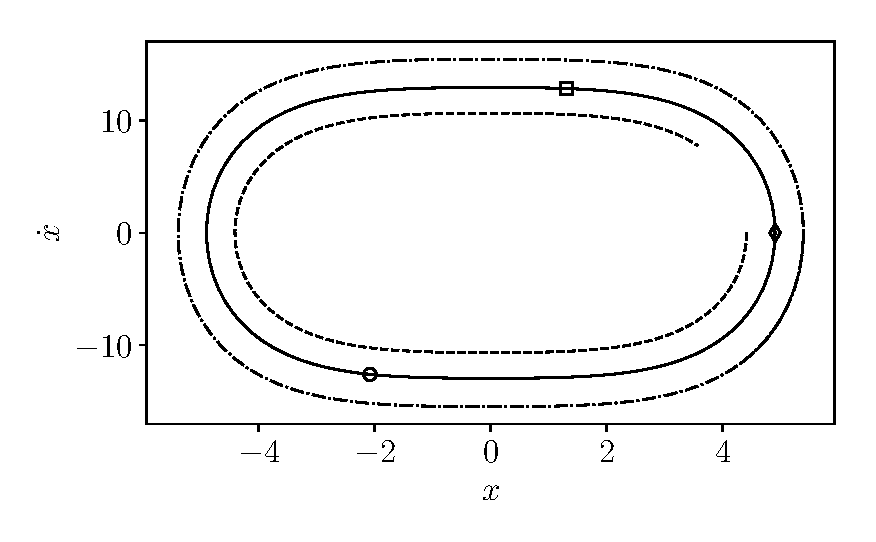
\includegraphics[width=\textwidth, height=5cm]{nnm/duff_per_space}
  \end{subfigure}
  \caption{Solution of the duffing eq. $\ddot x + x + 0.5x^3=0$ for different
    initial conditions and $T=2.0215$s.
    \textbf{(a)}: time series;
    \textbf{(b)}: phase space.
    Initial conditions for different line styles:
    \sampleline{}: [4.9009, 0];
    \sampleline{dashed}: 0.9$\cdot$[4.9009, 0];
    \sampleline{dotted}: 1.1$\cdot$[4.9009, 0];
    Markers represent different initial conditions for the periodic solution.
    $\diamond$: [4.9009, 0];
    $\square$: [1.308, 12.8764];
    $\circ$: [-2.0825, -12.6177]
  }
  \label{fig:sm_phase}
\end{figure}


In summary, the periodic solution is found by solving
\begin{equation}
  \label{eq:sm_bvp_problem}
  \bm h_{NNM} =
  \begin{bmatrix}
    \bm h(\bm z_{p}, T) = 0 \\
    g(\bm z_{p} ) = 0
  \end{bmatrix}
\end{equation}

The solution is found by corrections to the initial guess, done by
Newton-Raphson iterations. The shooting function is expanded in a Taylor series
% around increments $\Delta \bm z_{p0}$ and $\Delta T_{p0}$

\begin{equation}
  \label{eq:sm_nr}
  \bm h +
  \bm h_{\bm z} \Delta \bm z_{p} +
  \bm h_{T} \Delta T
  + H.O.T. = 0
  % Jeg har glemt mixede product herunder:
  %\mathcal{O}(\Delta \bm z_{p0}^2, \Delta T_{p0}^2) = 0
\end{equation}
where all terms are evaluated at $(z_0,T)$ and $H.O.T.$ the neglected higher
order terms. Thus the corrections are found by solving the linear equation

\begin{equation}
  \label{eq:sm_nr_sol}
  \begin{bmatrix}
    \bm h_{\bm z} & \bm h_{T} \\
    g_{\bm z} & 0
  \end{bmatrix}
  \begin{bmatrix}
    \Delta \bm z_{p} \\
    \Delta T
  \end{bmatrix}
  = -
  \begin{bmatrix}
    \bm h \\
    g
  \end{bmatrix}
\end{equation}

Since $\bm h_{NNM}$ have the transformation $\mathbb{R}^{2n+1} \rightarrow
\mathbb{R}^{2n+1}$ the Newton system is over determined, ie. the matrix to
invert is not square, and have to be solved in a least square sense.

The state is updated as

\begin{equation}
  \label{eq:sm_nr_update}
  \bm z^{k+1}_{p} = \bm z^k_{p} + \Delta \bm z^k_{p}, \quad
  T^{k+1} = T^k + \Delta T^k
\end{equation}
where $k$ is iteration number. The iteration is stopped when $\bm h_{nnm} = 0$
to some tolerance. Newmark-Raphson is a local algorithm. Convergence is
guarantied when the initial guess is close to solution, otherwise not. The
initial guess could for instance be the first linear mode and corresponding
period. If the Jacobian matrix $\bm J = [\bm h_{\bm z}, \bm h_T] $ is exact, the
convergence is second order.


The partial derivatives of the shooting function are found as:
\begin{align}
  \label{eq:sm_jac1}
  \bm h_{\bm{z}}&=
  \frac{\p \bm z(t, \bm z_0)}{\p \bm z_0}\bigg|_{t=T} - \bm I \\
  \bm h_T &=
  \frac{\p \bm z(t, \bm z_0)}{\p t}\bigg|_{t=T} =
  \bm h_{ham}(\bm z(T, \bm z_0))
  \label{eq:sm_jac2}
\end{align}
where $\bm h_{T}$ is a $2n$ vector, $\bm h_{\bm z_{0}}$ is $2n\times 2n$ matrix.


% The NR converges to a single solution depending on initial conditions. If
% It should be mentioned that for some forcing parameters, where a nonlinear
% system might have multiple solutions, the NR will, depending on the initial
% conditions, converge towards only one of them. Methods relying on the homotopy
% method or Groebner bases can be employed to find multiple solution - not that I
% know anything about these methods.

\subsubsection{Sensitivity analysis}
\label{sec:sm_sens_ana}

The Jacobian matrix $\p \bm z(t,\bm z_0) / \p \bm z_{0}$ from eq.
\eqref{eq:sm_jac2}, which represent the variation of the solution $\bm z(t,\bm
z_0)$ at time $t$ to pertubated initial conditions $\bm z_0$, is normally
calculated in two ways. Either by finite difference: successively pertubation of
each of the $2n$ initial condtion and integrating over the period. This is
computationally expensive and gives slower NR convergence since the Jacobi
matrix is only approximate.

Instead sensitivity analysis is used. The state space formulation
\eqref{eq:sm_state} is differentiated with respect to initial conditions $\bm
z_0$

\begin{align}
  &\frac{\p}{\p \bm z_0} \left[ \dot{\bm z}(t, \bm z_0) \right] =
    \frac{\p}{\p \bm z_0} \left[ \bm h_{ham}(\bm z) \right] \implies
  \nonumber \\
  &\frac{\d}{\d t} \left[  \frac{\p \bm z(t, \bm z_0)}{\p \bm z_0} \right] =
    \frac{\p \bm h_{ham}(\bm z)}{\p \bm z}\bigg|_{\bm z(t,\bm z_0)}
    \frac{\p \bm z(t, \bm z_0)}{\p \bm z_0}
    \label{eq:sm_sens}
\end{align}
with initial condition
\begin{equation}
  \label{eq:sm_sens_init}
  \frac{\p \bm z(0,\bm z_0)}{\p \bm z_0} = \bm I
\end{equation}
since $\bm z(0,\bm z_0) = \bm z_0$.

Then eq. \eqref{eq:sm_sens} is integrated over $T$ to obtain the Jacobian matrix
at time $t=T$. This integration is linear and carried out at the same time as
the Newmark integration of the periodic solution. In practise the eom
formulation eq. \eqref{eq:per_eom} is used for the sensitivity analysis. See
appendix \ref{sec:newmark_sens} for a derivation. The sensitivity analysis
requires the nonlinear forces to be smooth. If they are nonsmooth, finite
difference have to be used.

\subsubsection{Stability}
\label{sec:sm_stab}

The stability of a periodic solution is found from the Jacobian matrix evaluated
at $t=T$, called the \textit{monodromy matrix}

\begin{equation}
  \label{eq:sm_stab}
  \Phi = \frac{\p \bm z(t, \bm z_0)}{\p \bm z_0}\bigg|_{t=T}
\end{equation}
From it, it is determined whether a small initial perturbation decays or grows.
The stability is found from the eigenvalues $\sigma_i$ of $\Phi$, the Floquet
multipliers. If an Floquet multiplier is larger than one (i.e., $|\sigma_i|>
1$), the orbit is unstable. Conversely, the periodic orbit is stable if
$|\sigma_i| \leq 1, \forall i$

Equivalently the Floquet exponents $\lambda$ could be used. If there is at least
one Floquet exponents with a real part larger than 0 the solution is unstable.
They are related through the relation

\begin{equation}
  \label{eq:floquet_relations}
  \sigma_i = e^{\lambda_i T}
\end{equation}

Both variants are depicted on the complex plane and either compared to the unit
circle or the imaginary axis, respectively. See section \ref{sec:bifurcations},
fig \ref{fig:bifurcation} for a graphical representation.

\subsection{Harmonic balance}
\label{sec:harmonic_bal}

Where the shooting method finds a periodic solution by solving the system in
time domain, HB finds the periodic solution in frequency domain. The method is
described in \textcite{detroux2016a}.

A periodic solution to the damped and forced eom eq. \eqref{eq:per_eom} is
sought.
As the signal $\bm x$ and forces $\bm f(\bm x, \dot{\bm x}, \omega ,t) = \bm
p(\omega, t)- \bm f_{nl}(\bm x, \dot{\bm x})$ are assumed periodic, they are
approximated by Fourier series truncated to the $N_H$-th harmonic

\begin{align}
  \label{eq:hb_x_expansion}
  \bm x(t) &= \frac{\bm c^x_0}{\sqrt{2}} \sum_{k=1}^{N_H} (s^x_k \sin(k\omega t) +
          c^x_k \cos(k\omega t)) \\
  \label{eq:hb_f_expansion}
  \bm f(t) &= \frac{\bm c^f_0}{\sqrt{2}} \sum_{k=1}^{N_H} (s^f_k \sin(k\omega t) +
          c^f_k \cos(k\omega t))
\end{align}
where $\bm s_k$ and $\bm c_k$ represent the vectors of the Fourier coefficients
related to sine and cosine terms. The Fourier coefficients of the force $\bm f(t)$,
$\bm s^f_k$ and $\bm c^f_k$ depends on the Fourier coefficients of the
displacement $\bm x(t)$, $\bm s^x_k$ and $\bm c^x_k$ which are the new unknowns.
Gathering the coefficients into vectors

\begin{align}
  \label{eq:hb_coeffz}
  &\bm z =
    \begin{bmatrix}
      (\bm c^x_0)^T & (\bm s^x_1)^T & (\bm c^x_1)^T & \cdots &
      (\bm s^x_{N_H})^T & (\bm c^x_{N_H})^T
    \end{bmatrix}^T \\
  \label{eq:hb_coeffz}
  &\bm b =
    \begin{bmatrix}
      (\bm c^f_0)^T & (\bm s^f_1)^T & (\bm c^f_1)^T & \cdots &
      (\bm s^f_{N_H})^T & (\bm c^f_{N_H})^T
    \end{bmatrix}^T
\end{align}
then using a compact notion, the displacement and force is written as

\begin{align}
  \label{eq:hm_x_compact}
  &\bm x(t) = (\bm Q(t) \otimes \bm I_n) \bm z \\
  \label{eq:hb_y_compact}
  &\bm f(t) = (\bm Q(t) \otimes \bm I_n) \bm b
\end{align}
where $\otimes$ is the Kronecker product and $\bm Q$ a vector with harmonic terms

\begin{equation}
  \label{eq:hb_Q}
  \bm Q(t) =
  \begin{bmatrix}
    \frac{1}{2} & \sin(\omega t) & \cos(\omega t) & \cdots & \sin(N_H \omega t) &
    \cos(N_H \omega t)
  \end{bmatrix}
\end{equation}

Velocities and accelerations are found using the Fourier series as
\begin{align}
  \label{eq:hb_vel}
  &\dot{\bm x} = \left( \dot{\bm Q}(t) \otimes \bm I_n \right) \bm z =
    \left( (\bm Q(t) \bm \nabla) \otimes \bm I_n \right) \bm z \\
  \label{eq:hb_acc}
  &\ddot{\bm x} = \left( \ddot{\bm Q}(t) \otimes \bm{I}_n \right) \bm z =
    \left( (\bm Q(t) \bm \nabla^2) \otimes \bm{I}_n \right) \bm z \\
\end{align}

By substituting eqs. \eqref{eq:hb_x_expansion}-\eqref{eq:hb_f_expansion} and
\eqref{eq:hb_vel}-\eqref{eq:hb_acc} into the eom \eqref{eq:per_eom} and using a
galerkin procedure, one ends up with the equations of motion in frequency
domain (see appendix \ref{sec:hb_appendix} for more details on the derivation
and definition of $\bm \nabla$(the gradient as diagonal matrix))

\begin{equation}
  \label{eq:hb_feom}
  (\bm \nabla^2 \otimes \bm M)\bm z + (\bm \nabla \otimes \bm C)\bm z +
  (\bm{I}_{2N_H} \otimes \bm K)\bm z =
  (\bm{I}_{2N_H} \otimes \bm{I}_n )\bm b
\end{equation}
or in more compact form

\begin{equation}
  \label{eq:hb_feom_compact}
  \bm h(\bm z, \omega) = \bm A(\omega) \bm z - \bm b(\bm z) = \bm 0
\end{equation}
where $\bm A$ describes the linear dynamics

\begin{equation}
  \label{eq:hb_A}
  \bm A = \bm \nabla^2 \otimes \bm M + \bm \nabla \otimes \bm C +
  \bm{I}_{2N_H} \otimes \bm K
\end{equation}

If $\bm z$ is a solution of \eqref{eq:hb_feom_compact}, then the time signal $x^*$
constructed from $z^*$ is periodic and satisfies the eom \eqref{eq:per_eom}. As
with the shooting function, eq. \eqref{eq:hb_feom_compact} is nonlinear (due to
$\bm b$ dependence on $\bm z$) and have to be solved iteratively by
Newton-Rahpson iterations. It should however be noted that $\bm h(\bm z,
\omega)$ is an (nonlinear) algebraic equation, ie. there is no need for
time integration.

\begin{equation}
  \label{eq:hb_nr}
  \bm z^{(k+1)} = \bm z^{(j)} -
  \frac{\bm h(\bm z, \omega)}{\bm h_{\bm z}(\bm z, \omega)}
\end{equation}


\subsubsection{Expression of nonlinear terms and Jacobian matrix}
\label{sec:hb_exp_nonlin_jac}

Solution of eq \eqref{eq:hb_nr} requires calculation of $\bm H$ and of the
Jacobian matrix $\bm H_{\bm z}$, which in turn requires calculation of $\bm b$
and its derivatives.

It is not known how the Fourier coefficients in $\bm b$ relates to the
coefficients in $\bm z$, ie. it is not possible to directly calculate $\bm b(\bm
z)$ due to $\bm f_{nl}$ depends on $x$. Instead a technique called the
\textit{alternating frequency-time domain}(AFT) method is used. Here $\bm b$ is
calculated through successive Fourier transformations as shown in figure
\ref{fig:hb_aft}

\begin{center}
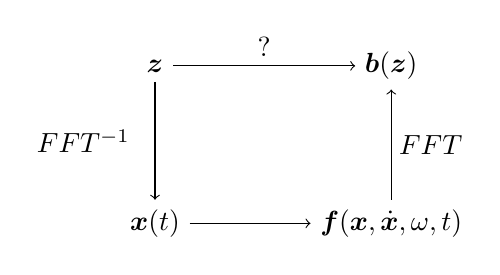
\begin{tikzpicture}[node distance=1.5cm]
  % nodes
  \node (A) at (0, 2) {$\bm z$};
  \node (B) at (0, 0) {$\bm x(t)$};
  \node (C) at (3, 0) {$\bm f(\bm x,\dot{\bm x},\omega, t)$};
  \node (D) at (3, 2) {$\bm b(\bm z)$};
  % arrows
  \draw [->]
  (A) edge node[anchor=center, text width=3.0cm] {$FFT^{-1}$} (B)
  (B) edge (C)
  (C) edge  node[anchor=center, text width=-0.2cm] {$FFT$} (D)
  (A) edge  node[anchor=center, above] {?} (D);
\end{tikzpicture}
\captionof{figure}{Graphical representation of the alternating frequency-time
  domain (AFT) method}
\label{fig:hb_aft}
\end{center}

$\bm x$ is calculated from the Fourier coefficients in $\bm z$, then the
nonlinear (and external) forces $\bm f$ are evaluated in time domain and $\bm b$
is found as the Fourier coefficients of $\bm f$.

The Jacobian matrix is given by
\begin{equation}
  \label{eq:hb_jac1}
    \bm h_{\bm z} = \frac{\p \bm h}{\p \bm z} = \bm A - \frac{\p \bm b}{\p \bm z}
\end{equation}
where the hard part is to compute $\bm b_{\bm z}$. The method for calculating
the Jacobian matrix follows the AFT method as well. To do that, the inverse
Fourier transform is written as the linear operator $\bm \Gamma(\omega)$

\begin{equation}
  \label{eq:hb_gamma}
  \begin{aligned}
    \bm \Gamma(\omega) =
    \left[
  \begin{matrix}
    \bm{I}_n \otimes
    \begin{bmatrix}
      1/\sqrt{2} \\ 1/\sqrt{2} \\ \vdots \\ 1/\sqrt{2}
    \end{bmatrix} &
    \bm{I}_n \otimes
    \begin{bmatrix}
      \sin(\omega t_1) \\ \sin(\omega t_2) \\ \vdots \\ \sin(\omega t_{t_N})
    \end{bmatrix} &
    \bm{I}_n \otimes
    \begin{bmatrix}
      \cos(\omega t_1) \\ \cos(\omega t_2) \\ \vdots \\ \cos(\omega t_{t_N})
    \end{bmatrix}&
        \cdots
  \end{matrix}
\right. \\
\left.
  \begin{matrix}
    \bm{I}_n \otimes
    \begin{bmatrix}
      \sin(N_H\omega t_{}) \\ \sin(N_H\omega t_2) \\ \vdots \\ \sin(N_H\omega t_{t_N})
    \end{bmatrix} &
    \bm{I}_n \otimes
    \begin{bmatrix}
      \cos(N_H\omega t_{}) \\ \cos(N_H\omega t_2) \\ \vdots \\ \cos(N_H\omega t_{t_N})
    \end{bmatrix}
  \end{matrix}
\right]
\end{aligned}
\end{equation}

which is used on the concatenated time series
\begin{equation}
  \label{eq:hb_time_series}
  \begin{aligned}
    \tilde{\bm x} =
    \begin{bmatrix}
      x_1(t_1) & \cdots & x_1(t_N) & \cdots & x_n(t_1) & \cdots & x_n(t_N)
    \end{bmatrix}^T\\
    \tilde{\bm f} =
    \begin{bmatrix}
      f_1(t_1) & \cdots & f_1(t_N) & \cdots & f_n(t_1) & \cdots & f_n(t_N)
    \end{bmatrix}^T
  \end{aligned}
\end{equation}

Thus the inverse and direct Fourier transform are written
\begin{equation}
  \label{eq:hb_four_transform}
    \tilde{\bm x} = \bm \Gamma(\omega) \bm z, \quad
    \bm z =( \bm \Gamma(\omega))^+ \tilde{\bm x}
\end{equation}
where $()^+$ is the Moore-Penrose pseduinverse since $\Gamma$ is not square. In
implementation the solution is found by a least square solver.

The Fourier coefficients of the external and nonlinear forces are then
\begin{equation}
  \label{eq:hb_b_coeff}
  \bm b(\bm z) = ( \bm \Gamma(\omega))^+ \tilde{\bm f}
\end{equation}
and the Jacobian is computed as
\begin{equation}
  \label{eq:hb_jac}
  \bm H_{\bm z} = \bm A - \frac{\p \bm b}{\p \bm z} =
  \bm A -
  \frac{\p\bm b}{\p \tilde{\bm f}}
  \frac{\p \tilde{\bm f}}{\p \tilde{\bm x}}
  \frac{\p \tilde{\bm x}}{\p \bm z} =
  \bm A - \bm \Gamma^+ \frac{\p \tilde{\bm f}}{\p \tilde{\bm x}} \bm \Gamma
\end{equation}

It should be noted that the concatenated time series vectors $\tilde{\bm x}$ and
$\tilde{\bm f}$ are newer used. They are only used in the derivation for the
expression for the Jacobian. Only the Fourier operator $\bm \Gamma$ and
extracted Fourier coefficients $\bm x$ are used.


\subsubsection{Stability}
\label{sec:hb_stab}

Unlike the shooting method (or general time domain methods), the monodromy
matrix is not readily available as a byproduct since there is no time
integration. Instead for frequency methods, \textit{Hills method} is used to
approximate the Floquet exponents by solving a quadratic eigenvalue problem
whose components are obtained as byproduct of the HB method.

Perturbing a periodic solution by an exponential decay
\begin{equation}
  \label{eq:hb_pert}
  \bm p(t) = \bm x(t) + e^{\lambda t}\bm s(t)
\end{equation}
and inserting this into the eom eq. \eqref{eq:per_eom} it is shown in appendix
\ref{sec:hb_stab_appendix} that the quadratic eigenvalue problem is found as

\begin{equation}
  \label{eq:hb_quad_eigen}
  \bm \Delta_2 \bm \lambda^2 + \bm \Delta_1 \bm \lambda + \bm h_{\bm z} = \bm 0
\end{equation}
where $\bm \Delta$ are matrices describing the linear dynamics similar to $\bm
A$ in eq. \eqref{eq:hb_A} and $\lambda$ are Hills coefficients.

The quadratic eigenvalue problem is rewritten to a linear eigenvalue problem of
double size

\begin{equation}
  \label{eq:hb_double_eigen}
  \bm B_1 - \gamma \bm B_2 = \bm 0
\end{equation}
where

\begin{equation}
  \label{eq:hb_stab_B12}
  \bm B_1 =
  \begin{bmatrix}
    \bm \Delta B_1 & \bm h_{\bm z} \\
    -\bm{I}    & \bm 0
  \end{bmatrix}, \quad
  \bm B_2 = -
  \begin{bmatrix}
    \bm \Delta_2   & \bm 0 \\
    \bm 0          & \bm{I}
  \end{bmatrix}
\end{equation}

The coefficients $\bm \lambda$ are found as the eigenvalues of the $(2N_H+1)2n$
square matrix

\begin{equation}
  \label{eq:hb_B}
  \bm B = \bm B^{-1}_2 \bm B_1 =
  \begin{bmatrix}
    -\bm \Delta^{-1}_2 \bm\Delta_1 & -\bm \Delta^{-1}_2 \bm h_{\bm z} \\
    \bm{I}                    & \bm 0
  \end{bmatrix}
\end{equation}
or from the generalised eigenvalueproblem eq. \eqref{eq:hb_stab_B12}.

Only $2n$ eigenvalues approximate the Floquet exponents $\tilde{\bm \lambda}$,
the rest are spurious. The ones needed are the $2n$ values with smallest
imaginary magnitude.

The diagonal matrix
\begin{equation}
  \label{eq:hb_B_tilde}
  \tilde{\bm B} =
  \begin{bmatrix}
    \tilde \lambda_1 \\
    & \ddots \\
    & & \tilde \lambda_{2n}
  \end{bmatrix}
\end{equation}
gathers the Floquet exponents identified from the $(2_{N_H} + 1)2n$ Hill's
coefficients. Besides stability, they are used for detecting bifurcations in
section \ref{sec:detecting_bifs}.

\subsubsection{Example}
\label{sec:hb_example}

Figure \ref{fig:hb_duffing_periodic} shows the periodic of the coupled duffing
Duffing system. Although the excitation is pure sine, the response contains
multiple harmonics due to nonlinearity. The normalized harmonic components are
found as

\begin{equation}
  \label{eq:hb_normal_coeff}
  \begin{aligned}
    \sigma_i = \frac{\phi_i}{\sum_{k=0}^{N_H} \phi_i}, \quad (i=0,\cdots, N_H) \\
    \phi_0 = \frac{c_0^x}{\sqrt{2}}, \quad \phi_i = \sqrt{(s^x_i) + (c^x_i)^2}
  \end{aligned}
\end{equation}

\begin{figure}[!ht]
  \centering
  \begin{subfigure}[b]{0.6\textwidth}
    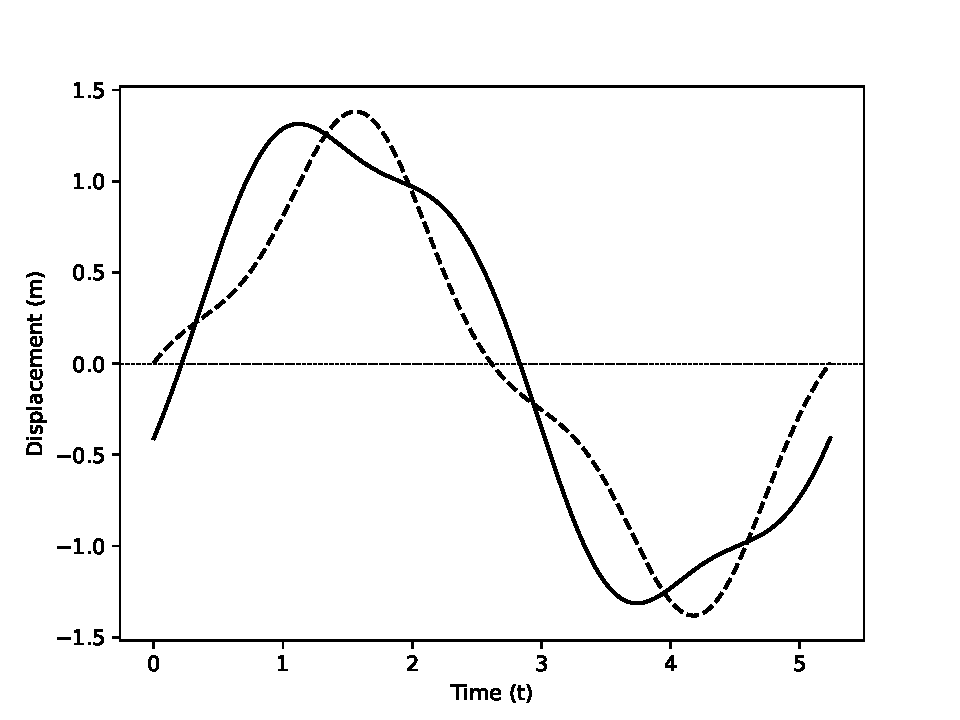
\includegraphics[width=\linewidth, height=6cm]{2dof_duffing/hb_per}
    \caption{}
  \end{subfigure}
  ~
  \begin{subfigure}[b]{0.36\textwidth}
    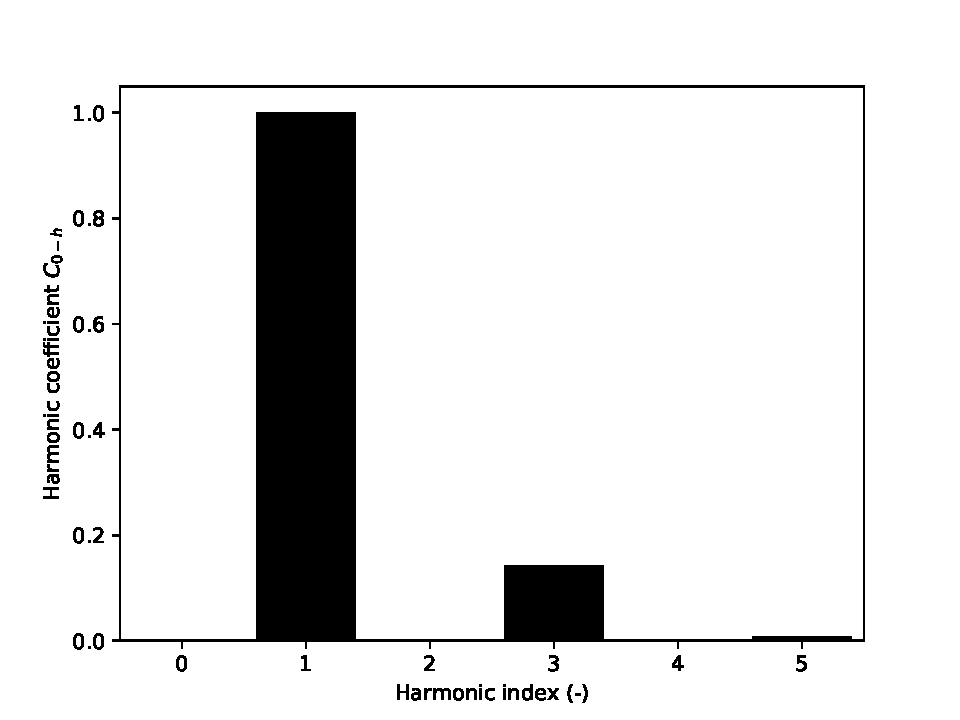
\includegraphics[width=\linewidth, height=6cm]{2dof_duffing/hb_har}
    \caption{}
  \end{subfigure}
    \caption{Periodic solution of the coupled Duffing system for $f=2$,
    $\omega=1.2$ and $N_H=5$.
    \textbf{(a)}: Time series;
    \textbf{(b)}: Normalized harmonic components of $x_1$.}
  \label{fig:hb_duffing_periodic}
\end{figure}
\FloatBarrier

\subsection{Summary}
\label{sec:per_summary}

Periodic solutions of nonlinear structures can be computed with
time-domain(shooting method) and frequency-domain(harmonic balance) methods. The
main difference is in the implementation complexity, computional complexity and
accuracy. Both methods can be used together with continuation and have ways to compute
stability analysis without much extra cost.

Summarising the shooting method
\begin{multicols}{2}
  Pro
  \begin{itemize}
  \item Accurate
  \item (all) Higher harmonics represented
  \end{itemize}
  \columnbreak
  Cons
  \begin{itemize}
  \item Many time integrations
  \item Slow for larger systems
  \end{itemize}
\end{multicols}
If the shooting method should be used for damped and forced motion, only the
state space formulation have to be changed. See appendix
\ref{sec:shooting_appendix} for the few changes.

Summarising the harmonic balance method
\begin{multicols}{2}
  Pro
  \begin{itemize}
  \item Fast
  \item Harmonic coefficients available
  \item Can be used for filtering, ie. by defining the number of harmonics in
    the solution.
  \end{itemize}
  \columnbreak
  Cons
  \begin{itemize}
  \item Less accurate
  \item High number of harmonic might be necessary. Need to check the
    contribution from last harmonics to ensure enough is included.
  \end{itemize}
\end{multicols}


Stability of a periodic solution can be assessed through  their Floquet
multipliers or exponents. When the Shooting method is used, they are found from
the monodromy matrix. When \gls{hb} is used, they are found from Hills matrix.


%%% Local Variables:
%%% mode: latex
%%% TeX-master: "../../report"
%%% End:



\section{Continuation}
\label{sec:continuation}

When the periodic solution is found, finding the successively periodic solutions
is done by continuation.

As with finding periodic solutions, there exist multiple schemes to do
continuation. A general continuation is formulated as $F(x)=0, \quad
F:\mathbb{R}^{m+1} \to \mathbb{R}^{m} $, ie. here the structure is $\bm z \in
\mathbb{R}^m$, $\omega \in \mathbb{R}^1$ and $F$ the algebraic problem for which
a solution is sought.

The most simple continuation method, where $\omega$ is used as independent
parameter and uniformly increased at each step fails at turning points. Instead
most continuation methods uses a length-wise curve parameter and a
predictor-corrector model. Starting from a known solution $\bm y_j = [\bm
z_{p0,(j)},\omega_{(j)}]^T$ the next periodic solution $\bm y_{j+1}$ is found as

\begin{itemize}
\item Tangent prediction, $\bm y_{(j+1)}^{1} = y_{(j)}+s\bm t_{(i)}$, where $s$
  is the step size and $\bm t$ the tangent.
\item Newton-like corrections - The type determines the continuation method.
\item Adaptive step control. Here a simple model using the convergence of the
  Newton iterations is used: $s = \frac{it_{opt}}{it_{NR}} s$, ie. the step is
  updated based on the defined optimal number of iterations versus the actual
  used number of iteration
\end{itemize}

The two methods used in this project are the pseudo-archlength continuation and
the Moore-Penrose continuation. The main difference is computional complexity.
With pseudo-archlength, each time a new point is found on the curve, the tangent
vector have to be computed anew. With the Moore-penrose corrector, the tangent
vector is also corrected and we save the explicit calculation of the tangent at
each new point.

The aim is to show that is no harder to use the Moore-penrose corrector. Formal
descriptions are found in \autocite{dhooge2003a}

\subsection{Procedure}
\label{sec:cont_procedure}

The tangent at a solution point $\bm y_{i}$ is
\begin{equation}
  \label{eq:cont_tangent}
  \begin{bmatrix}
    \bm J(\bm y_{(i)}) \\ \bm t^T_{(i-1)}
  \end{bmatrix}
  \bm t_{i}
  =
  \begin{bmatrix}
    \bm 0 \\ 1
  \end{bmatrix}
\end{equation}
where
\begin{equation}
  \label{eq:cont_J}
  \bm J(\bm y_{(i)}) =
  \begin{bmatrix}
    \bm H_{\bm z}(\bm y_{(i)}) & \bm H_{\omega}(\bm y_{(i)})
  \end{bmatrix}
\end{equation}

The last row in eq. \eqref{eq:cont_tangent} prevents the continuation from
turning back, $\bm t_{(i)}\bm t_{(i+1)}=1$. For the first tangent calculation it
is replaced by a row of ones, which impose the length of the tangent to 1; later
predictions $\bm t_{(i+1)}$ must be normalized.
The prediction is then

\begin{equation}
  \label{eq:cont_pred}
  \bm y^{(1)}_{(i+1)} = \bm y_{(i+1)} + s \bm t_i
\end{equation}

The corrections Pseudo-archlength and Moore-penrose are used with the shooting
method and harmonic balance, respectively. Convergence is achieved when
\begin{equation}
  \label{eq:cont_convergence}
  \frac{\norm{\bm h}}{\norm{\bm z}} < tol
\end{equation}

\subsubsection{Shooting methods}
\label{sec:shooting_cont}

For the pseudo-archlength corrections, a solution is sought in the perpendicular
direction of the prediction. The corrections are given by

\begin{equation}
  \label{eq:nnm_cont_corr}
  \begin{aligned}
    &\bm y^{(j+1)} = \bm y^{(j+1)} + \Delta \bm y =
    \bm y^{(j+1)} -\bm G^{-1}_{\bm y} \bm G
  \end{aligned}
\end{equation}
where the prediction subscripts have been omitted. We have
\begin{equation}
  \label{eq:nnm_cont_mat}
  \bm G(\bm y) =
      \begin{bmatrix}
      \bm H(\bm y) \\ \bm 0
    \end{bmatrix}, \quad
    \bm G_{\bm y}(\bm y) =
    \begin{bmatrix}
      \bm J(\bm y) \\ \bm t^T
    \end{bmatrix}
  \end{equation}
where correction superscripts have been omitted. After convergence to a
solution, the tangent is calculated and the algorithm continues.

\subsubsection{Harmonic balance}
\label{sec:hb_cont}


For the Harmonic balance method the nearest solution to the prediction is
sought. This is done by updating the tangent direction at each corrector
iteration. But first $\bm h_\omega$ in eq. \eqref{eq:cont_J} is given by
\begin{equation}
  \label{eq:hb_cont_Hw}
  \bm h_\omega = \frac{\p \bm A}{\p \omega} \bm z
\end{equation}

Using a optimisation variable $\bm v$, initialised as the prediction tangent
$\bm v^{(1)} = \bm t_{(i)}$, the Moore-penrose corrections are given by

\begin{equation}
  \label{eq:hb_cont_corr}
  \begin{aligned}
    &\bm y^{(j+1)} = \bm y^{(j+1)} + \Delta \bm y =
    \bm y^{(j+1)} -\bm G^{-1}_{\bm y} \bm G \\
    &\bm v^{(j+1)} = \bm v^{(j+1)} + \Delta \bm y =
    \bm v^{(j+1)} -\bm G^{-1}_{\bm y} \bm R
  \end{aligned}
\end{equation}
where the prediction subscripts have been omitted. We have
\begin{equation}
  \label{eq:hb_cont_mat}
  \begin{aligned}
    \bm G(\bm y, \bm v) =
    \begin{bmatrix}
      \bm H(\bm y) \\ \bm 0
    \end{bmatrix}, \quad
    \bm G_{\bm y}(\bm y, \bm v) =
    \begin{bmatrix}
      \bm J(\bm y) \\ \bm v^T
    \end{bmatrix} \\
      \bm R(\bm y, \bm v) =
  \begin{bmatrix}
    \bm J(\bm y) \bm v \\ \bm 0
  \end{bmatrix}
  \end{aligned}
\end{equation}
where correction superscripts have been omitted.

When convergence is reached the tangent is calculated as the normalized
correction of $\bm v$, $\bm t_{(j+1)} = \frac{\bm v}{\norm{\bm v}}$.

During the corrections eq. (\ref{eq:hb_cont_corr}-\ref{eq:hb_cont_mat}) $\bm H_{\bm
  z}$ is calculated, making stability analysis with Hills method cheap after
each solution is obtained.

\subsection{Example}
\label{sec:cont_example}

Figure \ref{fig:hb_frf_2dof} shows the NRFC for the coupled duffing using five
harmonic terms. That is enough to capture the harmonic components, as seen in
figure \ref{fig:hb_duffing_periodic}. If a lower number of harmonic were
included - only one and three terms would be relevant since even harmonics are
zero; it would required an even nonlinearity to generate even harmonics - the
superharmonic resonances at lower frequencies will not be captured. See appendix
\ref{sec:hb_appendix} where NRFCs are shown for different HB and continuation
parameters.

\begin{figure}[!ht]
  \centering
  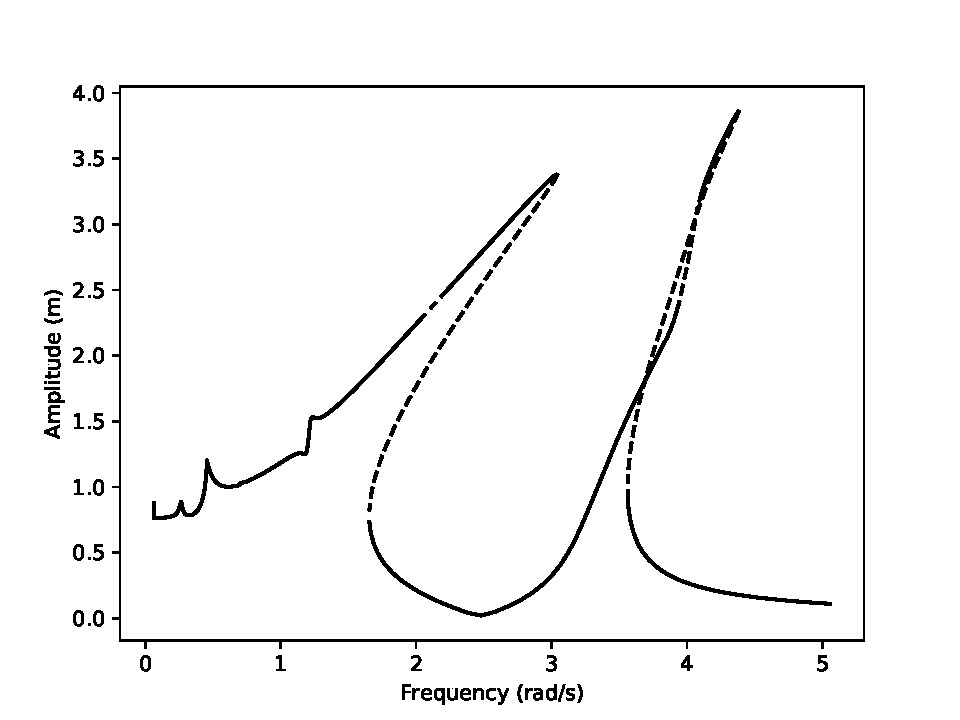
\includegraphics[width=0.7\linewidth, height=8cm]{2dof_duffing/hb_frf.pdf}
  \caption{NRFC of the coupled duffing system for $x_1$ with $f=2$N. Unstable
    branches are indicated by $- - -$. $N_H = 5, N = 512$}
  \label{fig:hb_frf_2dof}
 \end{figure}

\subsection{Summary}
\label{sec:cont_summary}

Figure \ref{fig:cont_algo} show the continuation procedure, regardless of the
the correction method. There is not much difference if implementation
complexity, but the Moore-penrose corrections saves on computional complexity.
The Pseudo-arclength method can be seen as a Moore-Penrose method for which the
correction direction is not updated.

\begin{figure}[!ht]
  \centering
  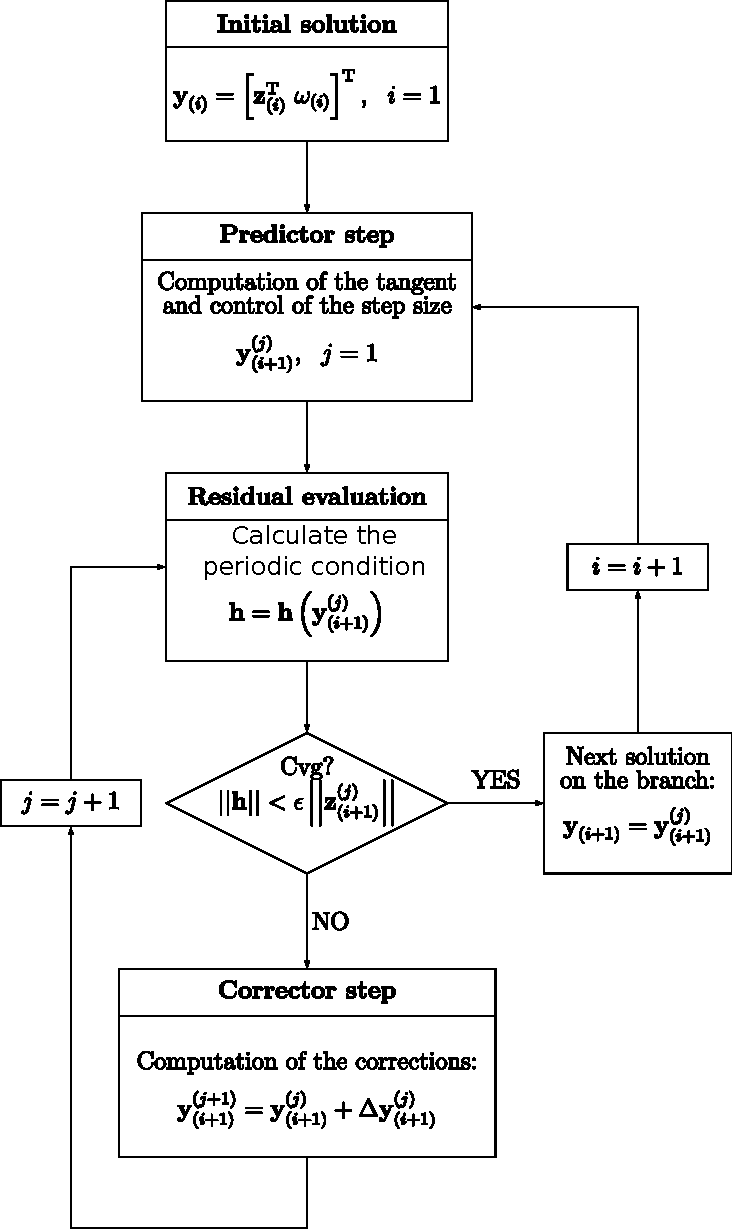
\includegraphics[width=0.7\textwidth]{continuation/continuation_diagram}
  \caption{Algorithm for Predictor-Corrector continuation of a periodic
    solution. For Moore-penrose the successive tangents are simply calculated as
  a normalization.}
  \label{fig:cont_algo}
\end{figure}



%%% Local Variables:
%%% mode: latex
%%% TeX-master: "../../report"
%%% End:


\section{Bifurcations}
\label{sec:bifurcations}

When stability of a periodic solution changes, it occurs at \textit{bifurcation
  points} in parameter space. At bifurcation points, the solution changes
qualitatively, but knowledge of the bifurcation type allows to predict the
behaviour. The type of bifurcation is related to how the Floquet multipliers
changes at said point, and the mechanism for loss of stability for the three
most common types are shown in figure \ref{fig:bifurcation}.

Bifurcations exist for multiple dimensions, but only codimension-1 bifurcations
are treated as only one parameter varies along the branch (ie. the forcing
frequency $\omega$). Bifurcations are a feature of nonlinear systems. Further
description is found in \textcite{juel2003a} or dedicated bifurcation textbooks
like \textcite{kuznetsov2013a}. Floquet multipliers $\sigma_i$ and Floquet
exponents $\lambda_i$ are related as (as restated from eq.
\eqref{eq:floquet_relations})

\begin{equation}
  \sigma_i = e^{\lambda_i T}
\end{equation}

\begin{figure}
  \centering
  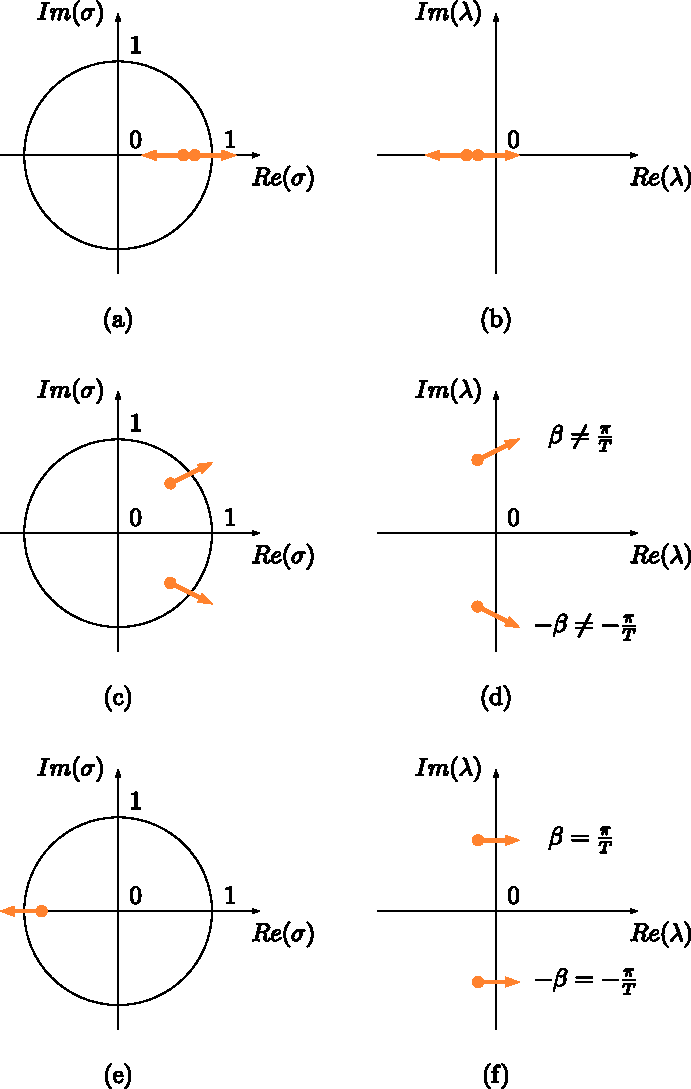
\includegraphics[width=0.7\textwidth]{bifurcation/bifurcation.pdf}
  \caption{Mechanisms for the loss of stability of a periodic solution,
    illustrated with Floquet multipliers (left column) and Floquet exponents
    (right column).
    \textbf{First row}: singular point;
    \textbf{Second row}: Neimark-Sacker bifurcation;
    \textbf{third row}: period doubling bifurcation.
    Reproduced from \parencite{detroux2016_phd}}
  \label{fig:bifurcation}
\end{figure}

\subsection{Fold and branch bifurcation Point}
\label{sec:singular_bif}

At fold point bifurcation point the state undergoes amplitude jumps and at
branch point bifurcation, branching, see below. These two types are detected when a Floquet
multiplier leaves the unit circle along the real axis through +1 or,
equivalently, when a Floquet exponent crosses the imaginary axis through 0, see
figs \ref{fig:bifurcation}(a,b)

At this point, the Jacobian matrix $\bm h_{\bm z}$ is singular: if $\bm h_{\bm
  z}$ is singular then the monodromy matrix $\bm \Phi$ of the Shooting method or
$\tilde{\bm B}$ of HB, eq \eqref{eq:hb_B}, is also singular and at least one
Floquet exponent is 0 (or a Floquet multiplier crosses the unit circle through
+1)


\begin{itemize}
\item \textit{Fold bifurcation} (also called Saddle node, Limit point or Turning
  point):\\
  The branch comes from one side and turns back, ie. the parameter($\omega$)
  increases and then decreases or decreases and then increases. Thus fold
  bifurcation indicates that there exist two solutions in its vicinity.
  It determines the upper or lower region of a bistable region and is often
  present in the vicinity of resonance peaks. This is the cause of amplitude
  jumps seen as response to stepped- or swept-sine excitation.
\item \textit{Branch bifurcation(BP)}: \\
  Two branches are connected. The two branches either meet and exchange
  stability (transcritical bifurcation), or one branch loses stability and a
  stable branch emanates from the point (pitchfork bifurcation).
\end{itemize}

Fold bifurcations satisfies
\begin{equation}
  \bm h_\omega \notin \text{range} (\bm h_{\bm z})
\end{equation}
whereas for BP
\begin{equation}
  \bm h_\omega \in \text{range} (\bm h_{\bm z})
\end{equation}

It follows that fold and BPs can be found, and distinguished, by
calculating the rank of the extended Jacobian $\bm J = [\bm h_{\bm z}| \bm
h_\omega]$ and $\bm h_{\bm z}$. If the rank of $\bm J$ is equal to $\bm h_{\bm
  z}$(and $\bm h_{\bm z}$ is singular) then it is a BP, otherwise fold.

If a BP is found, some branch switching mechanism should be used in the
continuation in order to switch branch. If no switching mechanism is used, the
continuation most likely continues on the same branch through the BP. The
new branch is found by calculating the two tangent directions at the BP;
thus some adoption of the predictor method is needed.


\subsection{Neimark-Sacker bifurcation}
\label{sec:ns_bif}

A Neimark-Sacker(NS) bifurcation (also called Hopf- or torus bifurcation) is
detected when a pair of Floquet multipliers leaves the unit circle as complex
conjugates or, equivalently, when a pair of Floquet exponent crosses the
imaginary axis as complex conjugates through any value but $\pm \frac{i\pi}{T}$,
where T is the period of oscillation, see figs \ref{fig:bifurcation}(c,d).

At NS a new type of oscillations emerges. These are called quasiperiodic
oscillations(QP) and despite the name they are not periodic. QPs contain the
forcing frequency $\omega$ (forcing), and at least another frequency
$\omega_2$(envelope). The two frequencies are incommensurate, ie.
$\frac{\omega}{\omega_2}$ is irrational. QP should not be confused with linear
beating, where the forcing frequency is close to the eigenfrequency $\omega_0$,
ie. $|\omega_0 - \omega|$ is small.

The imaginary part of the Floquet exponents that crosses the imaginary axis,
$\beta$, approximates the envelope pulsation $\omega_2$ of the QP in the
vicinity of the bifurcation, see fig. \ref{fig:bifurcation}(d)


\subsection{Period doubling bifurcation}
\label{sec:pd_bif}

A period doubling(PD) (also called flip bifurcation) is detected when a pair of Floquet
multipliers leaves the unit circle along the real axis through -1 or,
equivalently, when a pair of Floquet exponent crosses the imaginary axis as
complex conjugates through $\pm\frac{i\pi}{T}$, see figs.
\ref{fig:bifurcation}(e,f).

At PD a new branch of solution appears. The new branch have stable
periodic solutions with a doubled period. When they appear in cascade, PDs
can lead to chaos.


\section{Detecting bifurcations}
\label{sec:detecting_bifs}

To detect bifurcations during the continuation procedure, \textit{test
  functions} $\phi$ are monitored. When they change sign, a bifurcation is
detected. Each type of bifurcation have their own test function


\subsection{Fold and branch bifurcation Point}

As stated, fold and BP are characterised by rank deficiency of the
Jacobian matrix $\bm h_{\bm z}$. Thus a test function could be
\begin{equation}
  \phi_{F,BP} = \det{\bm h_{\bm z}}
\end{equation}
a computationally cheaper detection could be based on the monodromy or Hills
matrix, since this is already available
\begin{equation}
  \phi_{F,BP} = \det{\tilde{\bm B}}
\end{equation}

To distinguish between fold and BP, a dedicated test function is
\begin{equation}
  \phi_{BP} = \det
    \begin{pmatrix}
      \bm h_{\bm z} & \bm h_{\omega} \\
      \multicolumn{2}{c}{\bm t^T}
    \end{pmatrix}
\end{equation}

For detection fold bifurcation alone, a computationally cheaper way is to use
the geometric folding of the branch, ie. detect when the $\omega$ component of
the tangent prediction $\bm t$ changes sign,
\begin{equation}
  \phi_{F} = t_\omega
\end{equation}

\subsection{Neimark-Sacker and period doubling bifurcation}

NS and PD bifurcations, where a pair of Floquet exponents crosses the imaginary
axis as complex conjugates, can be detected using the \textit{bialternate
  product of a matrix} \autocite{kuznetsov2013a}. The bialternate product $\bm
P_\odot $ of a $m \times m$ matrix $\bm P$ is
\begin{equation}
  \bm P_\odot = 2\bm P \odot I_m
\end{equation}
with dimensions $m(m-1)/2$, is singular when two of its eigenvalues, $\mu 1$ and
$\mu 2$, verify:

\begin{equation}
  \mu_1 + \mu_2 = 0
\end{equation}
which is true for two purely imaginary- or real conjugate numbers. Thus the test
function is

\begin{equation}
  \phi_{NS,PD} = \det \left( \tilde{\bm B}_\odot \right)
\end{equation}
When the test function is zero, the Floquet exponents are checked. Two real
conjugates are associated with a neutral saddle point, which is not considered a
bifurcation and is ignored.
As a note: since $\tilde{\bm B}$ is diagonal, the bialternate product is also
diagonal.

\subsection{Calculating determinant efficiently}
\label{sec:bordering_tech}

Calculating the determinants needed for BP, NS and PD detection for large
scale structures might not be numerical stable. Instead the \textit{bordering
  technique} might be used, where the calculation of the determinant of $\bm G$
is replaced with calculation of a scalar function $g$ which vanishes at the same
time as the determinant \autocite{kuznetsov2013a}
\begin{equation}
  \begin{bmatrix}
    \bm G & \bm p \\
    \bm q^* & 0
  \end{bmatrix}
  \begin{bmatrix}
    \bm w \\ q
  \end{bmatrix}
  =
  \begin{bmatrix}
    \bm 0 \\ 1
  \end{bmatrix}
  \label{eq:bordered_system}
\end{equation}
where vectors $\bm p$ and $\bm q$ can be arbitrarily chosen as long as they
ensure nonsingularity of the system. This means they must be adapted or
recalculated along the branch to ensure good conditioning of the bordered
matrix.

$g$ is related to $\bm G$ by Cramer's rule
\begin{equation}
  g = \frac{\det
    \begin{pmatrix}
      \bm G & 0 \\
      \bm q^* & 1
    \end{pmatrix}}
  {\det
    \begin{pmatrix}
      \bm G & \bm p \\
      \bm q^* & 0
    \end{pmatrix}}
  =
  \frac{\det(\bm G)}
  {\det
    \begin{pmatrix}
      \bm G & \bm p \\
      \bm q^* & 0
    \end{pmatrix}}
\end{equation}


\subsection{Example}
\label{sec:bif_example}

The bifurcations for the coupled duffing system \eqref{eq:2dof} is shown in
figure \ref{fig:bif_example}. Fold, BP and NS bifurcations are found along the
branch. As expected fold bifurcations are found close to the two resonance
peaks. In fig. \ref{fig:bif_example}(b) a branch of periodic solutions emerges
from a BP bifurcation. In fig \ref{fig:bif_example}(c) QP oscillations appears
after a NS bifurcation.

\begin{figure}[ht!]
  \centering
    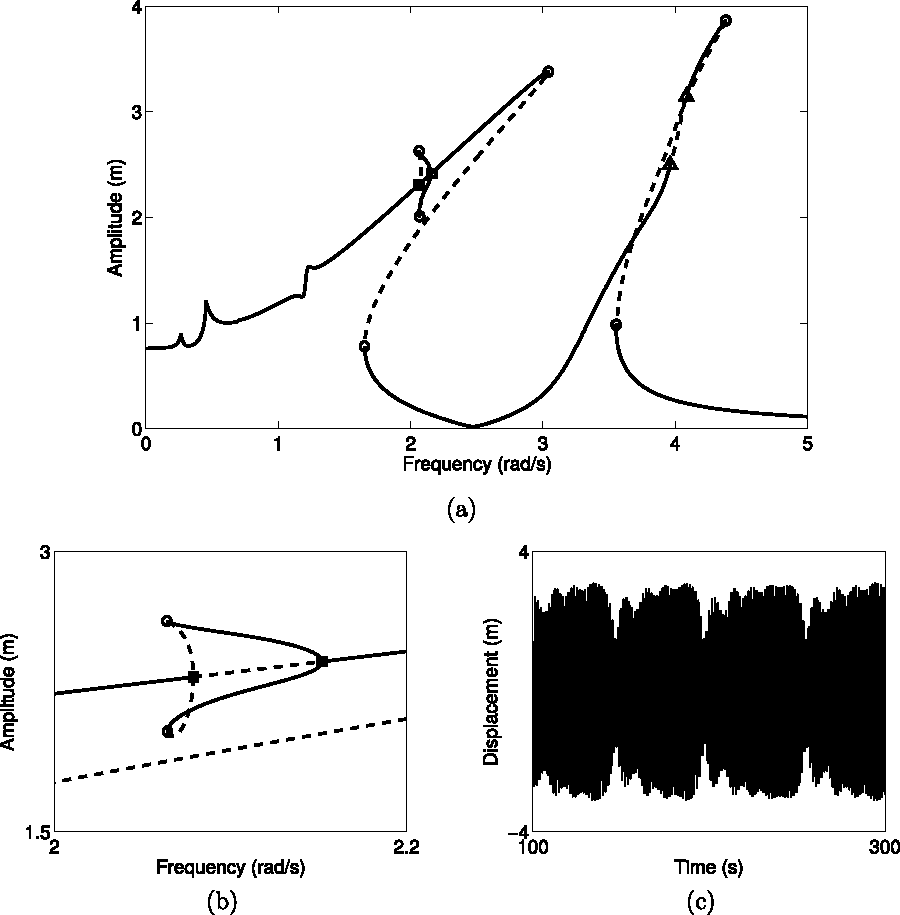
\includegraphics[width=0.85\textwidth]{bifurcation/bif_duffing.pdf}
  \caption{Bifurcation analysis of the coupled Duffing system at $x_1$ for
    $f=2$N.
    \textbf{(a)} Stable and unstable solutions are represented with solid and
    dashed lines. Fold, BP and NS bifurcations are represented with $\bm \circ$,
    $\bm \square$ and $\bm \triangle$ markers, respectively.
    \textbf{(b)} Close-up of the NRFC in the vicinity of the BPs and the
    emerging branch.
    \textbf{(c)} QP oscillations for a forcing frequency of $\omega=4$ rad/s.}
  \label{fig:bif_example}
\end{figure}

The evaluation of test functions for BP bifurcations along the branch is shown
in fig. \ref{fig:bif_BPtestfunction}. In fig \ref{fig:bif_BPtestfunction}(c) it
seen that the test function based on the determinant become very large close to
singular points whereas the bordering technique produce numerical stable values.

\begin{figure}[ht!]
  \centering
  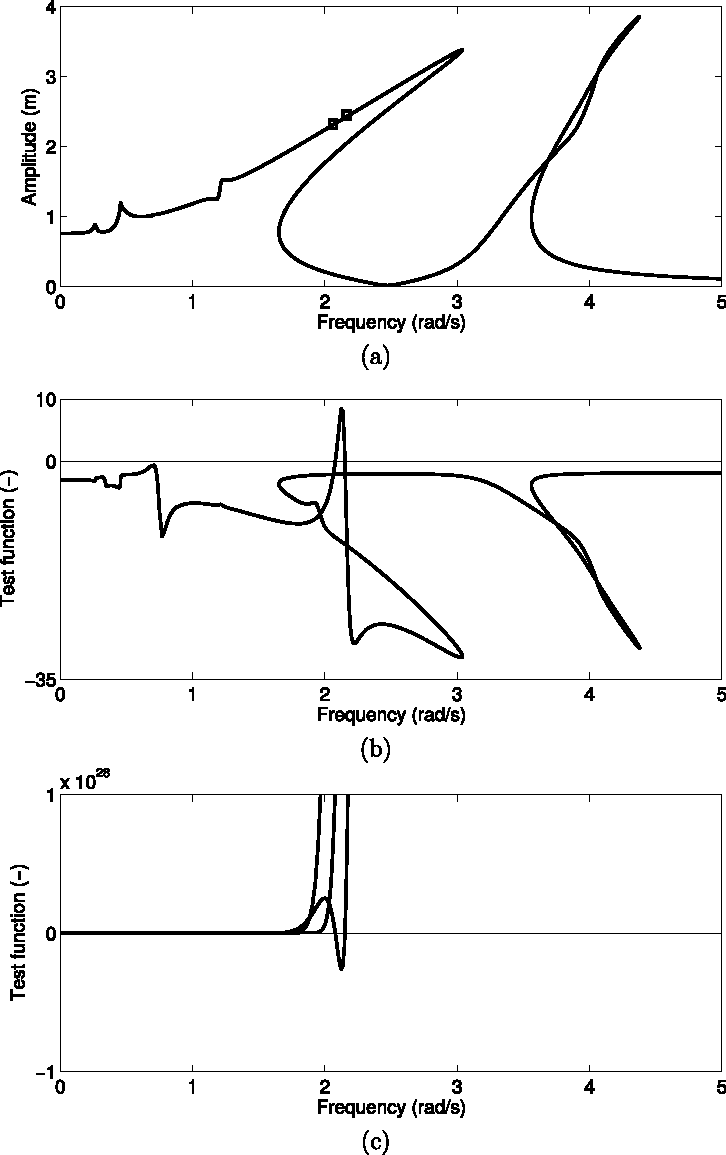
\includegraphics[width=0.85\textwidth]{bifurcation/test_funcBP.pdf}
  \caption{Test functions for BP detection.
    \textbf{(a)} NRFC and BP bifurcations marked by $\square$;
    \textbf{(b)} test function based on the bordering technique;
    \textbf{(c)} test function based on the determinant. It is noted that the
    determinant gets higher than $10^{28}$. The machine precision for a
    double precision 64 bit number is $\epsilon = 2^{-52} \sim 10^{-16}$,
    which means that the maximum spacing between two (normalised) numbers can be
    at max $2\epsilon |x|$ in order to be represented correct.}
  \label{fig:bif_BPtestfunction}
\end{figure}

\subsection{Summary}
\label{sec:bif_summary}

Bifurcation analysis can help understand nonlinear phenomena such as amplitude
jumps, quasiperiodic oscillations and period doubling. They are found during
continuation by using test functions; a summary is shown in fig
\ref{fig:bif_scheme} for Hills method.

\begin{figure}[ht!]
  \centering
 \begin{mdframed}
    \begin{enumerate}
    \item Detection of \textit{fold bifurcation}:\\
      \begin{equation*}
        \phi_F = t_{w}
      \end{equation*}
    \item Detection of \textit{bifurcation point} (BP):\\
      \begin{equation*}
        \phi_{BP} = g_{bp}
      \end{equation*}
      from the bordering system in eq. \ref{eq:bordered_system} with
      \begin{equation*}
        \bm G_{BP}
        \begin{bmatrix}
          \bm h_{\bm z} & \bm h_{\omega} \\
          \multicolumn{2}{c}{\bm t^T}
        \end{bmatrix}
      \end{equation*}
    \item Detection of \textit{Neimark-Sacker} (NS) and \textit{period doubling}
      (PD) bifurcations:\\
      \begin{equation*}
        \phi_{NS,PD} = g_{NS,PD}
      \end{equation*}
      from the bordering system in eq. \ref{eq:bordered_system} with $\bm
      G_{NS,PD} = \tilde{\bm B}_\odot$. When $\phi_{NS,PD} = 0$, matrix
      $\tilde{\bm B}$ has $\mu_1$ and $\mu_2$ among its eigenvalues, with
      \begin{equation*}
        \mu_1 + \mu_2 = 0
      \end{equation*}
      \begin{itemize}
      \item If $\mu_{1,2}=\pm i\beta$ with $\beta \neq \pi/T$, a NS
        bifurcation is detected.
      \item If $\mu_{1,2}=\pm i\beta$ with $\beta = \pi/T$, a PD bifurcation is
        detected.
      \item If $\mu_{1,2}=\pm \beta$ a neutral saddle point is detected.
      \end{itemize}
    \end{enumerate}
    \end{mdframed}
    \caption{Test functions for detection of codimensional-1 bifurcation of NFRCs}
    \label{fig:bif_scheme}
\end{figure}

%%% Local Variables:
%%% mode: latex
%%% TeX-master: "../../report"
%%% End:


\section{Nonlinear normal modes}
\label{sec:nonl-norm-modes}

The (numerical) calculations of NNMs were introduced in
\textcite{kerschen2009b}, using a shooting method and pseudo-archlength
continuation technique.

The shooting method requires substantial computational effort for larger FEM
structures. A method based on harmonic balance (HB) and continuation was
recently introduced in the review by Renson~ \autocite{renson2016a}, which, among several
benefits, reduces the computational burden. The HB method for NNMs originated
from \textcite{detroux2016a}. A method for calculating NNMs for nonconservative
systems, mentioned in the review and originating from \textcite{renson2014_phd},
will not be studied in this thesis.

This is because for simple (and weekly) damping mechanism, the damped dynamics
can often be interpreted based on the topological structure and bifurcation of
the NNMs of the underlying Hamiltonian(conservative) system,
\autocite[sec. 4]{renson2016a}

{\textbf A so far very incomplete description}

Modal features are often used to examine vibrating structures, and for linear
structures, the theory and practice is well established.

The chapter introduce the concept of nonlinear normal modes (NNM), stating with
a recap of linear normal modes (LNM). A more in-depth investigation and history
of NNMs can be found in \autocite{kerschen2009a} and the monograph \autocite[chap
2.]{vakakis2008a}.


\subsection{Linear normal modes}
\label{sec:linear-normal-modes}


Linear normal modes is a central part of linear vibration theory.

They have a clear physical interpretation: when a system vibrates at a mode, all
parts of the system moves sinusoidal with a fixed phase.
Further the mathematical properties of LNMs allow for decoupling of the
governing equations, i.e. a linear system vibrates as if it were made of
independent oscillators governed by the eigensolution. The invariance and modal
superposition comes from this decoupling:

\begin{itemize}
\item Invariance: If the motion is initiated on one specific LNM, the remaining
  LNMs remain quiescent for all time
\item Modal superposition: Free and forced vibrations can conveniently be
  expressed as linear combinations of individual LNM motions.
\end{itemize}

The theory and application of LNM is extensive and mature, including model
reduction (substructuring techniques \autocite{craig1968a}), experimental modal
analysis \autocite{ewins2000a}, finite element model updating (and
validating)\autocite{friswell1995a} and structural health monitoring
\autocite{doebling1996damage}.



For nonlinear system, attempts to apply linear analysis results at best in a
suboptimal design. NMM is an attempt to generalize to concept of normal modes to
nonlinear systems. NMM was first defined by Lyaponov, but today two definitions
of NMMs are generally used:

Targeting a nonlinear extension of LNMs, \autocite{rosenberg1966a} gave a
definition of NNMs, for an undamped system, as a {\textit vibration in unison of the
  system}, i.e. a synchronous periodic oscillation. This requires that all
points of the system reach their extreme values and pass through zero
simultaneous, allowing all displacements to be expressed in terms of a single
reference displacement.
From this it follows that in the configuration space of the system, the NNM
oscillation is represented by either a straight modal line (similar NNM) or a
modal curve (non-similar NNM).

Similar NNMs are analogous to linear normal modes, in the sense that their modal
lines do not depend on the energy of the free oscillation and space-time
separation of the governing equations of motion can still be performed; however
this type of NNMs is only realized when special symmetries occur, and are not
typical (generic) in nonlinear systems. More generic are non-similar NNMs, whose
modal curves do depend on energy; this energy dependence prevents the direct
separation of space and time in the governing equations of motion by means of
non-similar NNMs, which complicates their analytical computation.


Rosenbergs definition does not allow for internal resonance or damping.  The
latter was addressed by \autocite{shaw1993a}, who introduced the concept of {\textit
  damped NNM invariant manifold} to account for the fact that the free
oscillation of a damped nonlinear system is a non-synchronous, decaying motion.
Nothing more will be said about Shaws definition here, instead the reader can
refer to \autocite{renson2014_phd} for a numerical implementation of this
definition.

To account for internal resonance, i.e. some coordinates may vibrate faster than
others and the system no longer vibrates in unison, \autocite{kerschen2009a}
relaxed Rosenbergs definition to {\textit (not necessarily synchronous)
  time-periodic oscillation of a conservative system} and is the definition used
in this thesis.


Finally, with the present definition of NNMs, they have the following properties
related to nonlinear systems:

\begin{itemize}
\item {\textbf Frequency-energy dependence}\\
  One property of nonlinear systems is the frequency-energy dependence of their
  oscillations, e.g., through hardening or softening behaviors, and the FRF is
  no longer invariant.
  The evolution of NNMs along their backbone accounts for this dependence, as
  illustrated in Section {\textbf TODO}. In some cases, the evolution of the modal
  properties results in the localization phenomenon, where vibration energy gets
  localized in a specific part of the structure.
\item {\textbf Internal resonances}\\
  During a general motion of the system, NNMs may interact. In the presence of
  these interactions, NNMs with well-separated fundamental frequencies can
  exchange energy.

  To expand a bit: At low energies these modes may possess incommensurate
  linearized natural frequencies so they do not satisfy internal resonance
  conditions. Due to the energy dependence of their frequencies, however, at
  higher energies the same NNMs may become internally resonant, as their
  energy-dependent frequencies may become commensurate resulting in strong
  nonlinear modal interactions
\item {\textbf Relations with forced responses}\\
  For structures with low damping, the NNM backbone traces the locus of the
  resonance peaks.
\end{itemize}

They might also provide insight into when linear analysis can be used and not.



As an example, consider the nonlinear 2DOF mass and spring system shown in
figure \ref{fig:2dof_system}.

\begin{figure}[!ht]
  \centering
  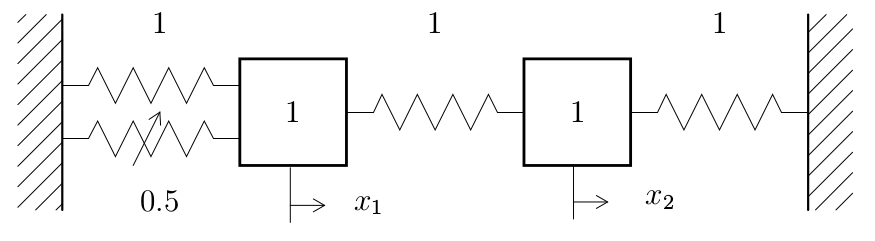
\includegraphics[width=0.7\textwidth]{nnm/2dof_system}
  \caption{Schematic representation of the 2DOF system}
  \label{fig:2dof_system}
\end{figure}

The equations of motion (EOM) are given by

\begin{equation}
  \label{eq:2dof_nonlin_sys}
  \begin{aligned}
    \ddot x_1 + (2x_1 - x_2) + 0.5 x_1^3 &= 0 \\
    \ddot x_2 + (2x_2 - x_2) &= 0
  \end{aligned}
\end{equation}

Note that this system is not symmetric so it possess only non-similar NNMs.


The underlaying linear system is given by

\begin{equation}
  \label{eq:2dof_lin_sys}
  \begin{aligned}
    \ddot x_1 + (2x_1 - x_2) &= 0 \\
    \ddot x_2 + (2x_2 - x_2) &= 0
  \end{aligned}
\end{equation}

The initial condition that excites the two linear modes of system
\eqref{eq:2dof_lin_sys} is found from the eigensolution, i.e. the two
eigenvectors.


Figure \ref{fig:nonlin_time_series} and \ref{fig:nonlin_nnm_config} shows the
time series and configuration plane for in-phase and out-of-phase NNMs for the
nonlinear system. The system vibrates in unison, even though higher harmonics
are present as seen by the curved modal lines in the configuration plot.


\begin{figure}[!ht]
  \centering
  \begin{subfigure}[b]{0.45\textwidth}
    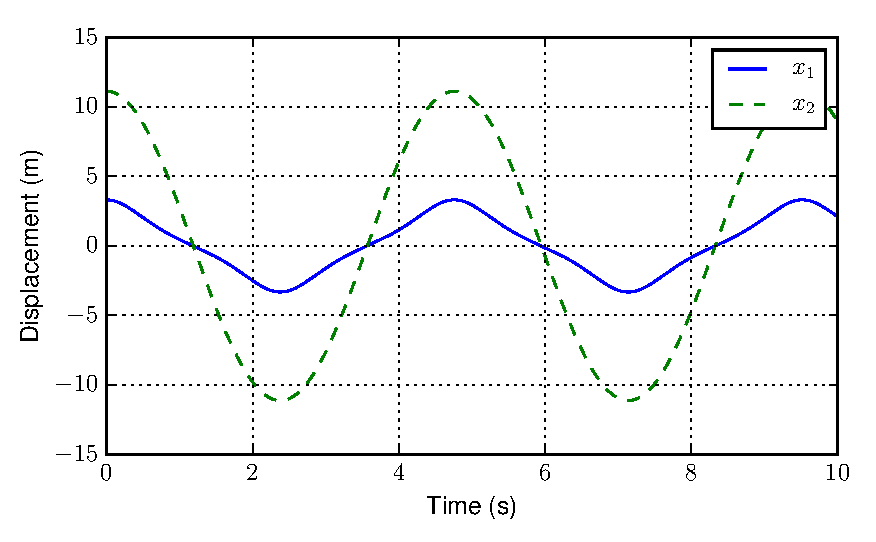
\includegraphics[width=\textwidth]{nnm/nonlin_inphase_time_hist}
  \end{subfigure}
  ~
  \begin{subfigure}[b]{0.45\textwidth}
    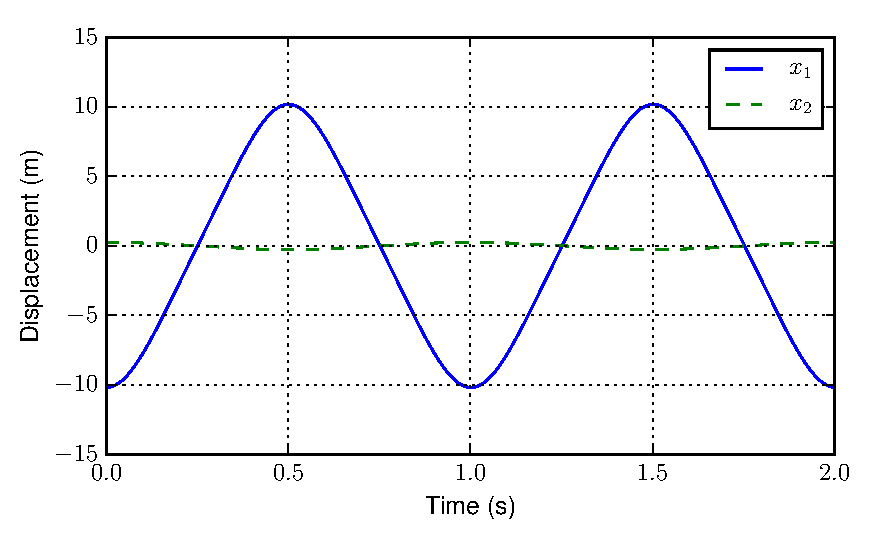
\includegraphics[width=\textwidth]{nnm/nonlin_outphase_time_hist}
  \end{subfigure}
  \caption{Time series of system (\ref{eq:2dof_nonlin_sys}).
    Left plot: in-phase NNM,
    $[x_1(0), x_2(0), \dot x_1(0), \dot x_2(0)] = [3.319, 11.134,0,0]$;
    Right plot: out-of-phase NNM,
    $[x_1(0), x_2(0), \dot x_1(0), \dot x_2(0)] = [-10.188, 0.262,0,0]$.}
  \label{fig:nonlin_time_series}
\end{figure}

\begin{figure}[!ht]
  \centering
  \begin{subfigure}[b]{0.45\textwidth}
    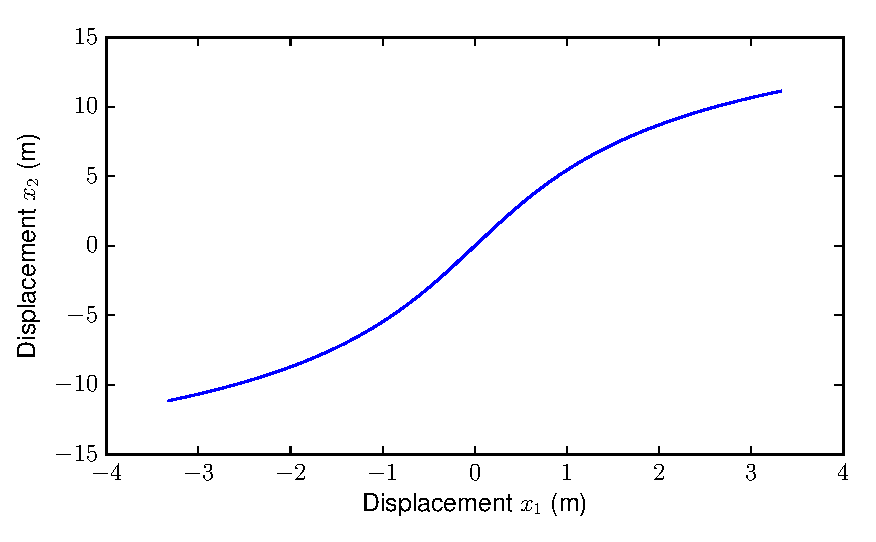
\includegraphics[width=\textwidth]{nnm/nonlin_inphase_conf_space}
  \end{subfigure}
  ~
  \begin{subfigure}[b]{0.45\textwidth}
    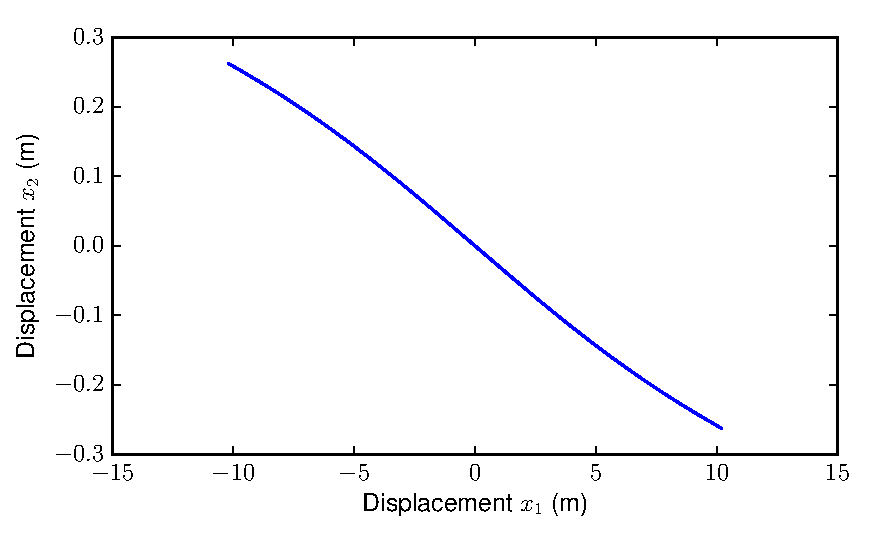
\includegraphics[width=\textwidth]{nnm/nonlin_outphase_conf_space}
  \end{subfigure}
  \caption{NNM motion of system (\ref{eq:2dof_nonlin_sys}) in configuration space.
    Left plot: in-phase NNM;
    Right plot: of-phase NNM.}
  \label{fig:nonlin_nnm_config}
\end{figure}



Figure \ref{fig:nonlin_3:1_int_resonance} shows internal 3:1 resonance. The
motion is still periodic, but not unison.

\begin{figure}[!ht]
  \centering
  \begin{subfigure}[b]{0.45\textwidth}
    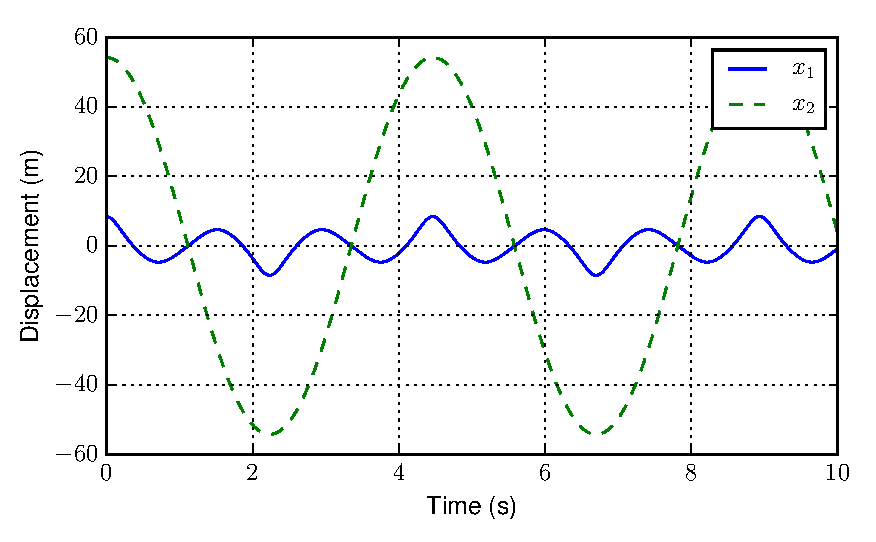
\includegraphics[width=\textwidth]{nnm/nonlin_31_time_hist}
  \end{subfigure}
  ~
  \begin{subfigure}[b]{0.45\textwidth}
    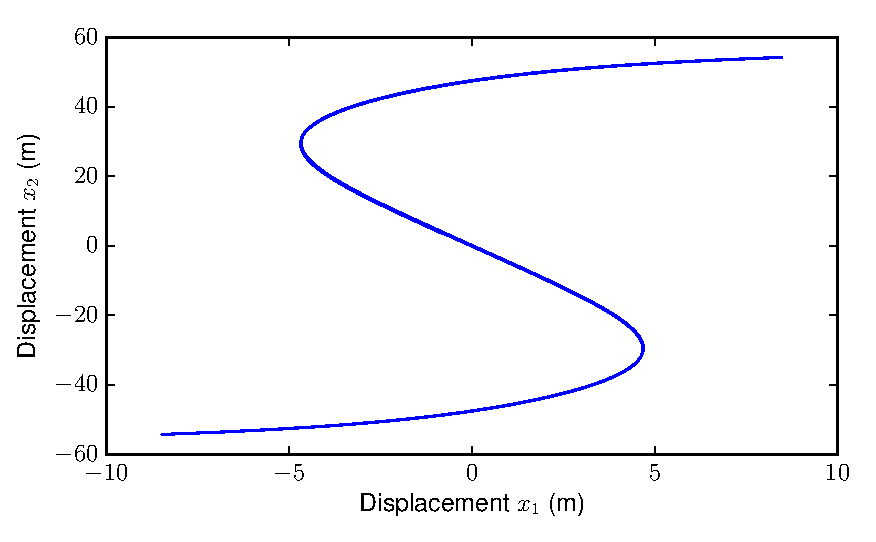
\includegraphics[width=\textwidth]{nnm/nonlin_31_conf_space}
  \end{subfigure}
  \caption{Internally resonant NNM of system \eqref{eq:2dof_nonlin_sys} (3:1
    resonance);
    $[x_1(0), x_2(0), \dot x_1(0), \dot x_2(0)] = [8.476, 54.263, 0, 0]$;
    Left plot: time series;
    Right plot: configuration space}
  \label{fig:nonlin_3:1_int_resonance}
\end{figure}




\subsection{Similar NNM, an example}
\label{sec:similar-nnm-an}


An example of similar NNMs are given in \autocite{vakakis1992a}.
Given the symmetric system

\begin{align}
    \ddot x_1 + k_3(x_1 - x_2)^3 + x_1 + x_1^3&= 0 \nonumber \\
    \ddot x_2 - k_3(x_2 - x_2)^3 + x_2 + x_2^3&= 0 \label{eq:2dof_similar_sys}
\end{align}
where $k_3$ is the strength of the nonlinear coupling.
This system possesses only similar NNMs (due to the symmetry), which are found
by imposing the functional relationship

\begin{equation}
  \label{eq:nnm_similar_relation}
  x_2 = c x_1
\end{equation}

where $c \in \Re$ is a real modal constant. Substituting
\eqref{eq:nnm_similar_relation} into \eqref{eq:2dof_similar_sys} to get a
algebraic equation satisfied by the modal constant

\begin{equation}
  \label{eq:nmm_similar_modal}
  k_3(1+c)(c-1)^3 = c(1-c^2)
\end{equation}

From figure \ref{fig:nnm_similar_bifur} it is seen that the system always
possesses the NNMs $x_2 = \pm x_1$ regardless of the coupling strength. This
correspond to the in-phase and out-of-phase similar NNMs respectively and can
be regarded as as a continuation of the two normal modes of the corresponding
linear system.


\begin{figure}[!ht]
  \centering
  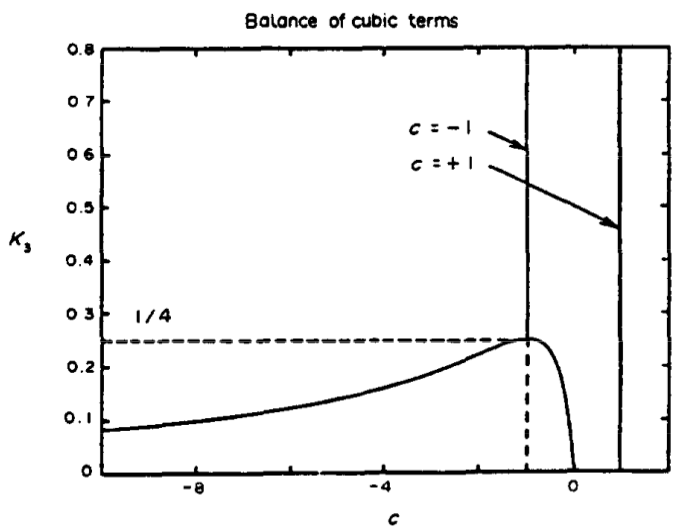
\includegraphics[width=0.7\textwidth]{nnm/similar-nnm-bifur}
  \caption{Pichfork bifurcation of NMMs. (---) stable mode, (- - -) unstable
    mode. From \autocite{vakakis1992a}}
  \label{fig:nnm_similar_bifur}
\end{figure}


However at $k_3 = 1/4$, the out-of-phase NNM bifurcates. The bifurcating NNMs are
out-of-phase, time-periodic motions of system and becomes strongly localized as
$k_3 \to 0$, i.e. one node vibrates strongly while the other stands still. This
shows another concept of NNM which differs from LNM: NNMs of a dynamical system
may exceed in number its degrees of freedom. Additionally, NNM bifurcations may
result in mode instability.


Figure \ref{fig:similar_time_series} shows the time series for out-of-phase NNMs
for \eqref{eq:2dof_similar_sys}, and figure \ref{fig:similar_nnm_config} shows
the corresponding configuration space. For the bifurcated NNM, localization is
seen. The system still vibrates with a single harmonic in unison, as seen by the
straight line in configuration space and the time series.

\begin{figure}[!ht]
  \centering
  \begin{subfigure}[b]{0.45\textwidth}
    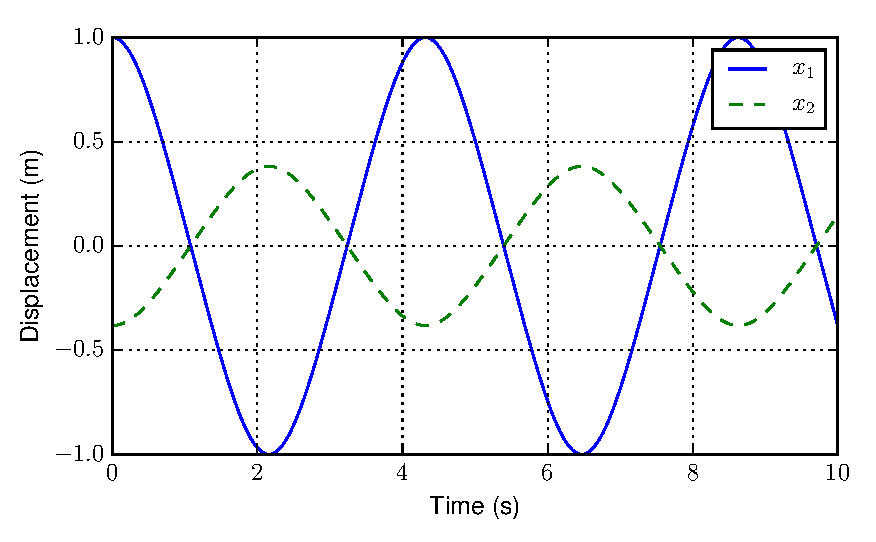
\includegraphics[width=\textwidth]{nnm/similar1_time_hist}
  \end{subfigure}
  ~
  \begin{subfigure}[b]{0.45\textwidth}
    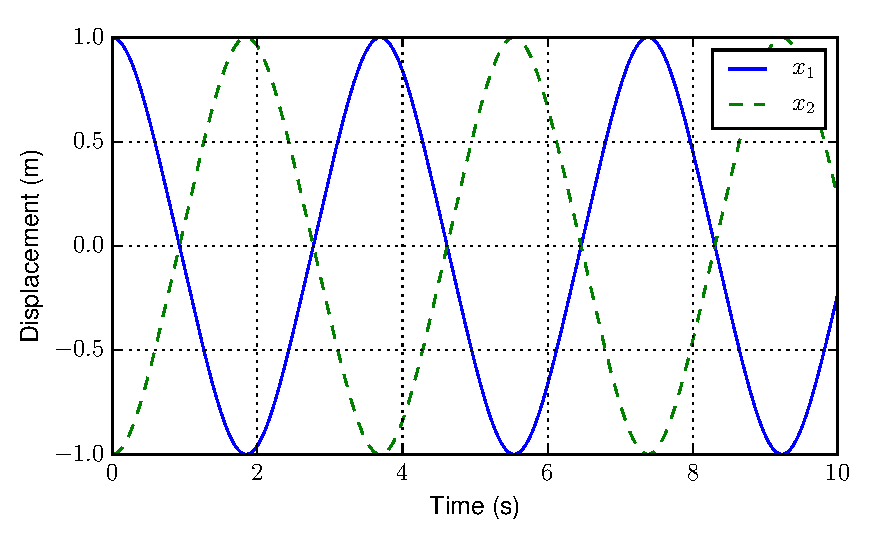
\includegraphics[width=\textwidth]{nnm/similar2_time_hist}
  \end{subfigure}
  \caption{Time series of system \eqref{eq:2dof_similar_sys}.
    Left plot: out-of-phase NNM, $k_3=0.2$,
    $[x_1(0), x_2(0), \dot x_1(0), \dot x_2(0)] = [1,-1,0,0]$;
    Right plot: out-of-phase NNM, $k_3=0.2$,
    $[x_1(0), x_2(0), \dot x_1(0), \dot x_2(0)] = [1, -0.3820,0,0]$.}
  \label{fig:similar_time_series}
\end{figure}


\begin{figure}[!ht]
  \centering
  \begin{subfigure}[b]{0.45\textwidth}
    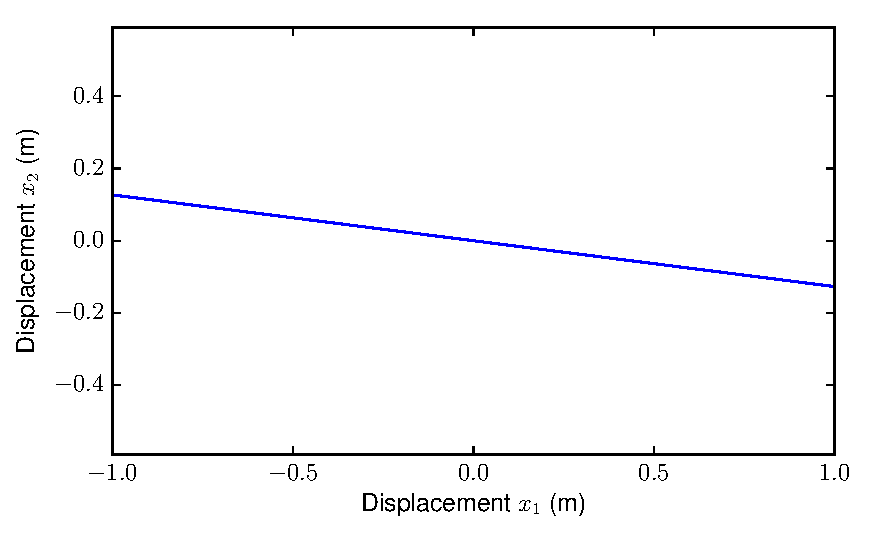
\includegraphics[width=\textwidth]{nnm/similar1_conf_space}
  \end{subfigure}
  ~
  \begin{subfigure}[b]{0.45\textwidth}
    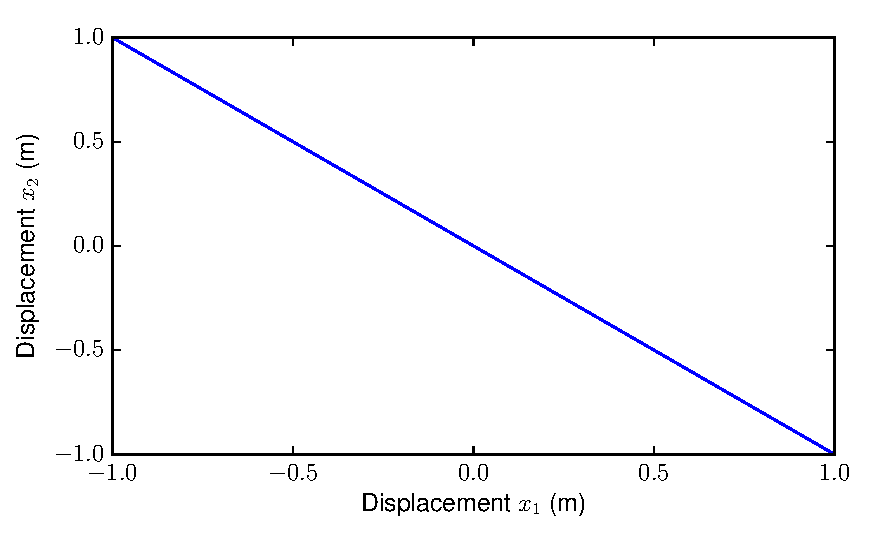
\includegraphics[width=\textwidth]{nnm/similar2_conf_space}
  \end{subfigure}
  \caption{NNM motion of system \eqref{eq:2dof_similar_sys} in configuration space.
    Left plot: out-phase NNM;
    Right plot: out-of-phase NNM.}
  \label{fig:similar_nnm_config}
\end{figure}


%%% Local Variables:
%%% mode: latex
%%% TeX-master: "../../report"
%%% End:

% -*- coding: utf-8 -*-

\chapter{Signal treatment}
\label{cha:signal-treatment}

Signal treatment and excitation type affects how the nonlinearity is seen in the
measured signal.
This chapter treats the types of excitation that are applicable for nonlinear
dynamics.

\section{Types of excitation}
\label{sec:types-excitation}

Different types of excitation gives different response for nonlinear structures,
with certain types being superior for detecting and characterizing and others
smooths out the nonlinearities. For a more in-depth treatment see
\textcite{gatto2010flexible}.


\begin{itemize}
\item \textit{steady state sine excitation}:\\
  Generally {\textit steady state sine excitation} (or {\textit stepped sine}), gives
  the most distinctive nonlinear effects. All the input energy is contained in
  the frequency of excitation. Noise can be removed from the signal by numerical
  filtering and integration, giving a good signal-to-noise ratio (SNR) and thus well
  defined FRFs with clear nonlinear distortions.
  
  The drawback of stepped sine is that it is slow compared to transient and
  random methods. At each step, time is required before the response attains
  steady state condition. It is the preferred method in literature when treating
  nonlinear behavior.

\item \textit{Impact excitation}:\\
  {\textit Impact excitation}, with hammer testing is the standard for measuring
  linear FRFs in industry. Because of the easiness of applying the test {\textit in
    situ} and the broad frequency content in the impulse excites a high number
  of modes.

  For nonlinear testing, the method is not well suited. The energy of each
  individual frequency is small, making it hard to excite structural
  nonlinearities.

\item \textit{random excitation}:\\
  FRFs obtained by band limited {\textit random excitation} will often appears
  linearized due to the randomness of the amplitude and phase of the excitation
  signal.

  \textbf{Lidt forklaring af det!} As for the impact excitation, the energy of
  each frequency is low, making it hard to drive structures into their nonlinear
  regime.

\item \textit{pseudo-random}:\\
  pseudo-random signal is a sum of multiple sine waves, with constant amplitude
  and the phase randomly selected from a uniform distribution between $180
  \degreeC$ and $-180 \degreeC$

  \begin{equation}
    \label{eq:multiple-sine}
    u(t) = \sum_{k=1}^{N_s} A_K \cos \left( 2 \pi k f_0 + \phi_k \right)
  \end{equation}

  where $N_k$ is the number of sine components, $A_k$ and $\phi_k$ is the
  amplitude and random phase of sine component $k$ and $f_0$ is the fundamental
  frequency. Time series of pseudo random signal is obtained by applying the
  inverse DFT to the generated frequency domain representation of the signal.

  To avoid transient effects delay blocks are used, ie. acquisition only starts
  after repeating the same excitation block a number of times.

  The FRF is not distorted by leakage or windowing and due to the continuous
  excitation, the signal has a high SNR.
\end{itemize}



% \section{Signal treatment}
% \label{sec:signal-treatment}

% \subsection{Differentiation}
% \label{sec:differentiation}

% Differentiation is hard without obtaining noisy results. Standard use of
% difference formulas, like the five-point central difference here, will result in noisy signals

% \begin{equation}
%   \label{eq:central_difference}
%   y_i = \frac{1}{12 \Delta t} \left( -y_{i+2} + 8y_{i+1} - 8y_{i-1} + y_{i-2} \right)
% \end{equation}



%%% Local Variables:
%%% mode: latex
%%% TeX-master: "../report"
%%% End:


\chapter{Implementation}
\label{cha:implementation}


The methods presented in the previous chapters are implemented as a library in
python and available online \autocite{paw2017}. The code depends on the standard
python libraries numpy, scipy and matplotlib and can run on all operating
systems. Care have been taking in order to ensure correctness of the
implementations; as much as it have been possible examples from papers and data given
from Liege have been recalculated to ensure that the same results were obtained.
All code is written for this thesis and implement most notably:
\begin{itemize}
\item FEM code: generate FE matrices $\bm M, \bm K$ from a \textit{gmsh}-mesh
  file. Different types of elements are available. Boundary conditions are
  enforced on system matrices.
\item Nonlinear newmark integration with sensitivity analysis
\item Morlet wavelet
\item Restoring force surface
\item Integration, filtering and periodicity calculation of signals
\item NNM continuation and stability
\item HB continuation, stability and bifurcation
\item FNSI, linear and nonlinear parameter estimation. Stabilisation diagram
  for determining model order
\item FRF calculation from periodic signals with multiple periods or from
  nonperiodic signals using spectral densities. Standard deviation of FRF
  between periods is calculated.
\item Modal properties including MAC calculation.
\item Sine sweep(linear and logarithmic) and random periodic excitation.
\item Polynomial and piecewise cubic splines available for identification.
\item Additional types of nonlinearities available for simulation with Newmark,
  HB and NNM: Piecewise linear and hyperbolic tangent(tanh), the latter only for
  damping.
\end{itemize}

As an example of the library approach, the following two examples shows how FNSI
identification and HB continuation are done. Most methods returns a class
storing all information, making multiple runs with different settings easy. To
keep the examples short, they are run with default settings.

\begin{lstlisting}[language=Python,frame=single,breaklines=true,basicstyle=\tiny]
from numpy import np
from vib.signal import Signal
from vib.fnsi import FNSI
from vib.nlforce import NL_force, NL_polynomial
from vib.common import modal_properties

# load time signal
# nsper is the number of signals per period, iu the dof(s) where the force(s) works
mat = np.load(filename + '.npz')
u, ydd, fs, nsper, iu = mat['u'], mat['ydd'], mat['fs'], mat['nsper'], mat['iu']

# create class, integrate and select period(s) (fnsi works on displacements)
signal = Signal(u, fs, ddy=ddy)
signal.get_displ(lowcut, highcut)
signal.cut(nsper, per=[7,8])

# setup nonlinear type and where it works (-1: attached to ground)
inl = np.array([[0,-1], [1,-1]])
enl = np.array([3,3])
nl_pol = NL_polynomial(inl, enl)
nl = NL_force().add(nl_pol)
fmin, fmax = 0, 10
ims, nmodel = 22, 4
fnsi = FNSI(signal, nl, fmin, fmax)
fnsi.calc_EY()
fnsi.svd_comp(ims)
fnsi.id(nmodel)
# Get identified nl parameters and linear frf.
knl, H, He = fnsi.nl_coeff(iu)
# get linear modal parameters
modal = modal_properties(fnsi.A, fnsi.C)
# Done.
\end{lstlisting}
and for HB:

\begin{lstlisting}[language=Python,frame=single,breaklines=true,basicstyle=\tiny]
import numpy as np
from vib.hb.hb import HB
from vib.hb.hbcommon import hb_signal
from vib.nlforce import NL_force, NL_polynomial

# setup system
M = np.array([[m1,0],[0,m2]])
C = np.array([[c1,0],[0,c2]])
K = np.array([[k1+k2, -k2],[-k2, k2+k3]])
inl = np.array([[0,-1], [1,-1]])
enl = np.array([3,3])
knl = np.array([mu1, mu2])
nl_pol = NL_polynomial(inl, enl, knl)
nl = NL_force()
nl.add(nl_pol)
# starting frequency, force amplitude and force dof
f0, famp, fdof = 1, 3, 0

# create HB class, periodic solution and continuation incl stability and
# bifurcation.
hb = HB(M,C,K,nl)
omega, z, stab, lamb = hb.periodic(f0, famp, fdof)
hb.continuation()

# Run for another forcing level
hb2 = HB(M,C,K,nl)
hb2.periodic(f0, 2*famp, fdof)
hb2.continuation(bifurcation=False)
# Done
\end{lstlisting}

All the examples from the previous chapters are included in the examples
directory in the source code, and should run on any python3 installation.

It is noted that the functionality of this library correspond to the Ni2D
software by Nolinsys, a company founded by researches at Liege University, and
should run at the same speed. The python library includes \textit{all} methods
included by Ni2D. The notable difference is that Ni2D have a graphical interface
and requires, besides a license to Ni2D, a license to matlab. The python library
does however have a interactive graphical interface for selecting RFS and
inspecting the evolution of \{stability changes, ie. Floquet exponents, harmonic
components and periodic solution\}(not shown in this report); both are inspired
by Ni2D.


%%% Local Variables:
%%% mode: latex
%%% TeX-master: "../report"
%%% End:


\chapter{Application}
\label{cha:application}

This chapter present two more involved cases of identification. The first case
is identification of the COST beam, introduced as a standard test case for
polynomial nonlinearities, ie. two polynomial nonlinearities at the same DOF.
The second case demonstrate the usage of cubic spines to identify a system with
two different clearances. The clearance distances are also found.


\section{COST beam}
\label{sec:cost-beam}

The European action COST F3 nonlinear beam \autocite{GOLINVAL2003} was
introduced in 2003 as a benchmark system for nonlinear vibrations. The
experimental setup is shown in fig. \ref{fig:beam_setup} and consists of a
clamped beam with a thin beam part at the end of the main beam.

\begin{figure}[!ht]
  \centering
  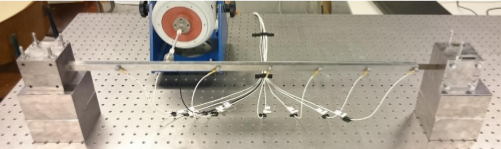
\includegraphics[width=0.7\textwidth]{nlbeam/beam_setup.png}
  \caption{Experimental setup for the COST beam. The setup is vertical to avoid
    gravitational effects which cannot be ignored due to the thin beam.}
  \label{fig:beam_setup}
\end{figure}


Accelerations are measured evenly along the beam at seven locations and excited
at node two.
From \textcite{lenaerts2003a} is it known that the system exhibit a (geometric)
cubic nonlinearity due to large deformations of the thin beam and quadratic
nonlinearity due to the clamped connection, both located at the tip of the main
beam. Using data given at the Nolinsys course, the beam will be identified as an
example of a MIMO system. After successful identification a FE model is built
using the identified parameters, and used for further examination.


\subsection{Identification}

The time series were obtained by Nolinsys. The beam is excited with a periodic
broadband input with flat amplitude spectrum, i.e. a multisine at low and high
level. At low and high level, the beam behaves linear and nonlinear
respectively. To avoid leakage in the identification due to transient behavior,
the periods used are selected from a plot of the periodicity. From fig.
\ref{fig:nlbeam_per} is seen that transients are apparent in the first two
periods and not apparent in periods 4-7, which are used for the identification.

\begin{figure}[!ht]
  \centering
  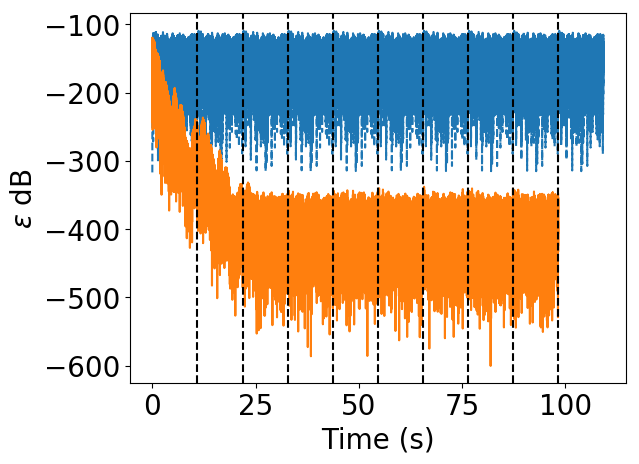
\includegraphics[width=0.6\textwidth]{nlbeam/fnsi/per.png}
  \caption{Periodicity of recorded signal at high level wrt. the last period.
    Measured at the nonlinear dof.}
  \label{fig:nlbeam_per}
\end{figure}

Figure \ref{fig:nlbeam_stab} shows the stabilisation diagram used for determine
model order. Fig. \ref{fig:nlbeam_stab}(a) is used for linear identification and
is fully stabilised at order 6. Fig. \ref{fig:nlbeam_stab}(b) shows the
nonlinear system identified with linear analysis, ie. without specifying
nonlinear basis functions. The first mode does not stabilise, which normally
indicates that the supplied basis functions are inadequate to represent the
nonlinearity. Fig. \ref{fig:nlbeam_stab}(c) shows the stabilisation after
supplying a quadratic and cubic basis function. The first mode stabilises at
model order 6, ie. the identification is most likely trustworthy and the
nonlinearity are described by these functions.

\begin{figure}
  \centering
    \begin{subfigure}[b]{0.45\textwidth}
      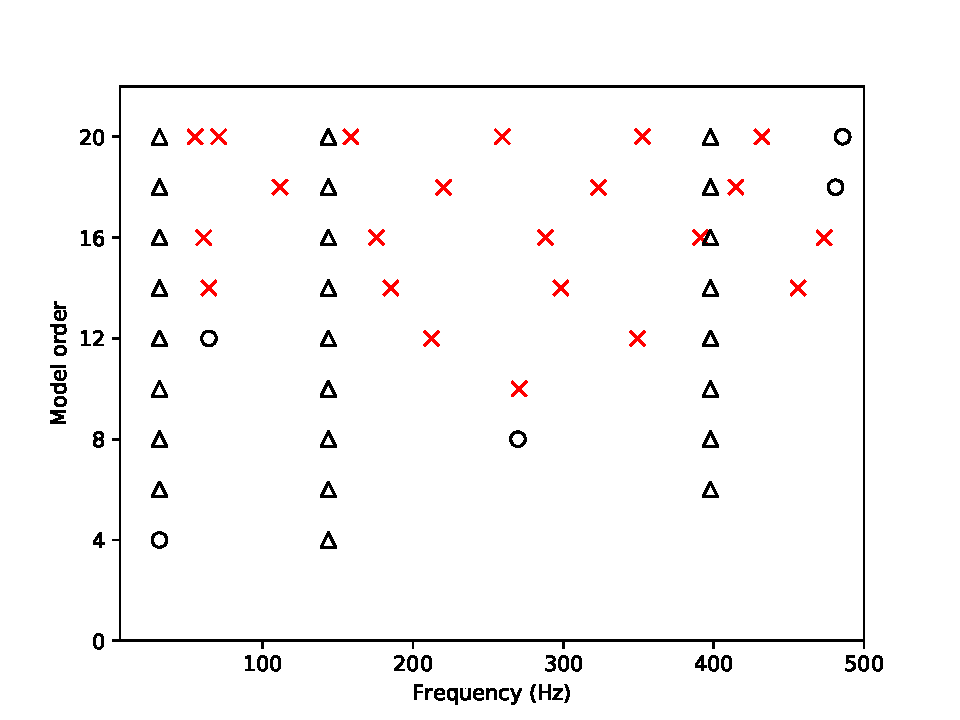
\includegraphics[width=\linewidth]{nlbeam/fnsi/stab_lin.pdf}
      \caption{}
    \end{subfigure}
    ~
    \begin{subfigure}[b]{0.45\textwidth}
      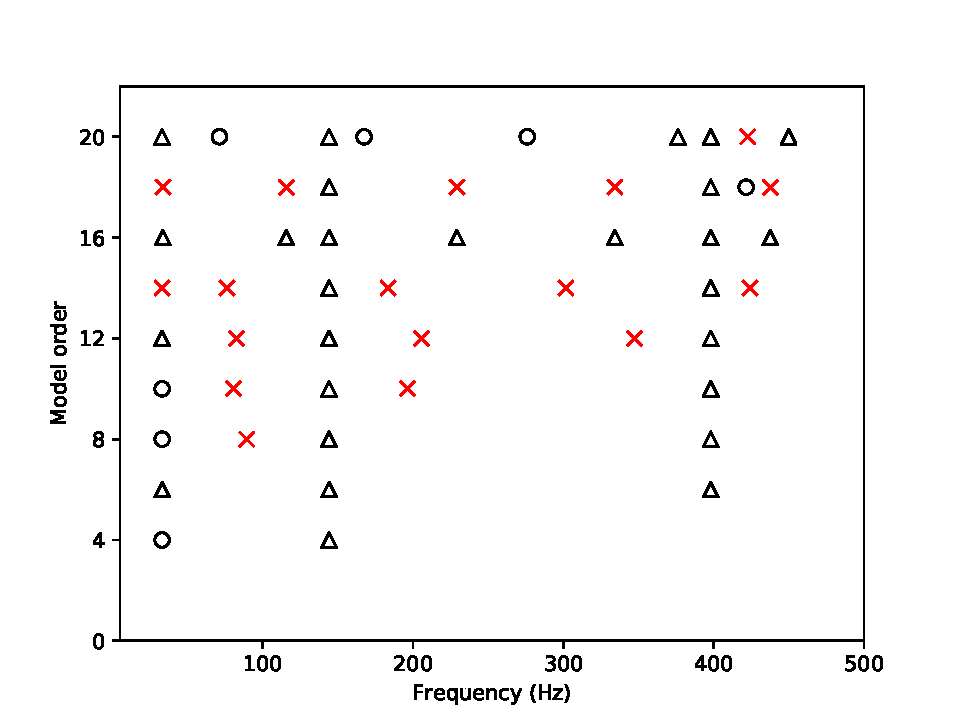
\includegraphics[width=\linewidth]{nlbeam/fnsi/stab_nlin1.pdf}
      \caption{}
    \end{subfigure}
    \\
    \begin{subfigure}[b]{0.45\textwidth}
      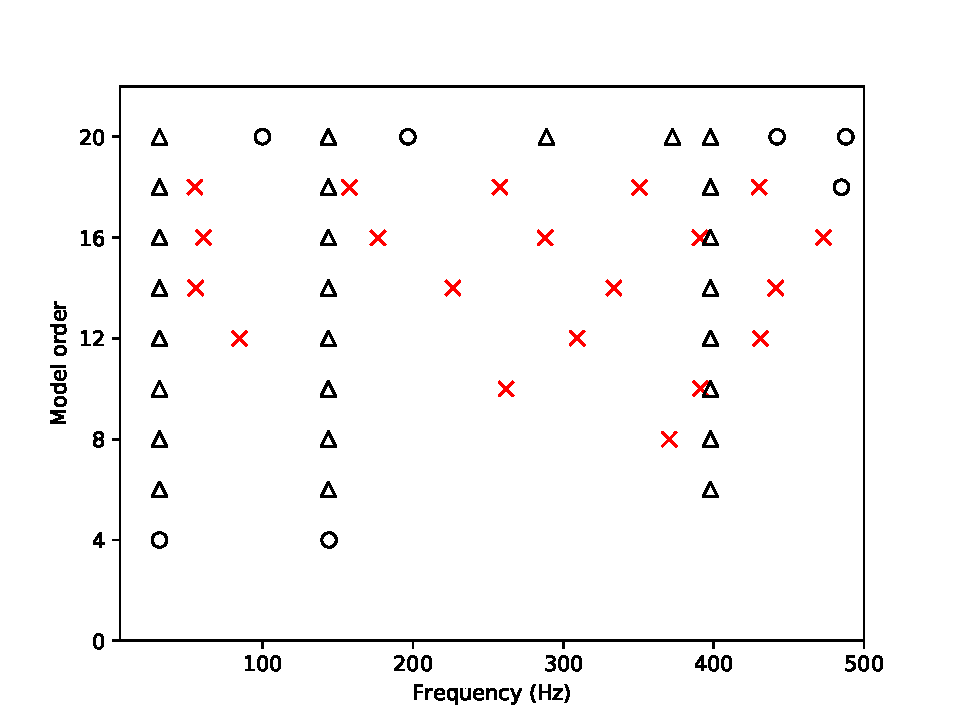
\includegraphics[width=\linewidth]{nlbeam/fnsi/stab_nlin2.pdf}
      \caption{}
    \end{subfigure}
    \caption{Estimation of model order.
    \textcolor{red}{$\pmb\times$}: new pole;
    $\pmb\circ$: extra stabilisation in MACX;
    $\pmb\triangle$: full stabilisation.
    \textbf{(a)}: Low level, linear identification;
    \textbf{(b)}: High level, linear identification - no stabilisation of first mode;
    \textbf{(c)}: High level, nonlinear identification - stabilisation of first mode;
  }
  \label{fig:nlbeam_stab}
\end{figure}

The identified linear parameters are shown in table \ref{nlbeam_par}. As
expected, the first mode shows a hardening which is seen by the linear
identification at high level. The linear parameters are estimated correctly at
high level using the two basis functions.

\begin{center}
  \begin{tabular}{*{4}{c}}
    \hline
    Mode & Frequency (Hz) & Damping ration (\%) & Deviation from linear freq. (\%) \\
    \hline
    1 & 31.3 & 1.27 \\
    2 & 143.6 & 0.29 \\
    3 & 397.8 & 0.14 \\
    \hline
    1 & 33.1 & 1.08 & 5.7 \\
    2 & 144.1 & 0.29 & 0.3 \\
    3 & 398.0 & 0.14 & 0.05 \\
    \hline
    1 & 31.3 & 1.27 & $10^{-3}$ \\
    2 & 143.6 & 0.29 & $10^{-5}$ \\
    3 & 397.8 & 0.14 & $10^{-6}$ \\
    \hline
  \end{tabular}
  \captionof{table}{Estimated linear natural frequencies and damping ratios for
    the COST beam.
    \textbf{(upper)}: Low level, linear identification;
    \textbf{(middle)}: High level, linear identification;
    \textbf{(lower)}: High level, nonlinear identification.
  }
  \label{tab:nlbeam_par}
\end{center}

The identified nonlinear coefficients are shown in figure \ref{fig:nlbeam_knl}.
The deviation of the real part is just within 1\% and the imaginary part are
around three orders of magnitude smaller, indicating a good identification.

\begin{figure}[!ht]
  \centering
  \begin{subfigure}[b]{0.45\textwidth}
    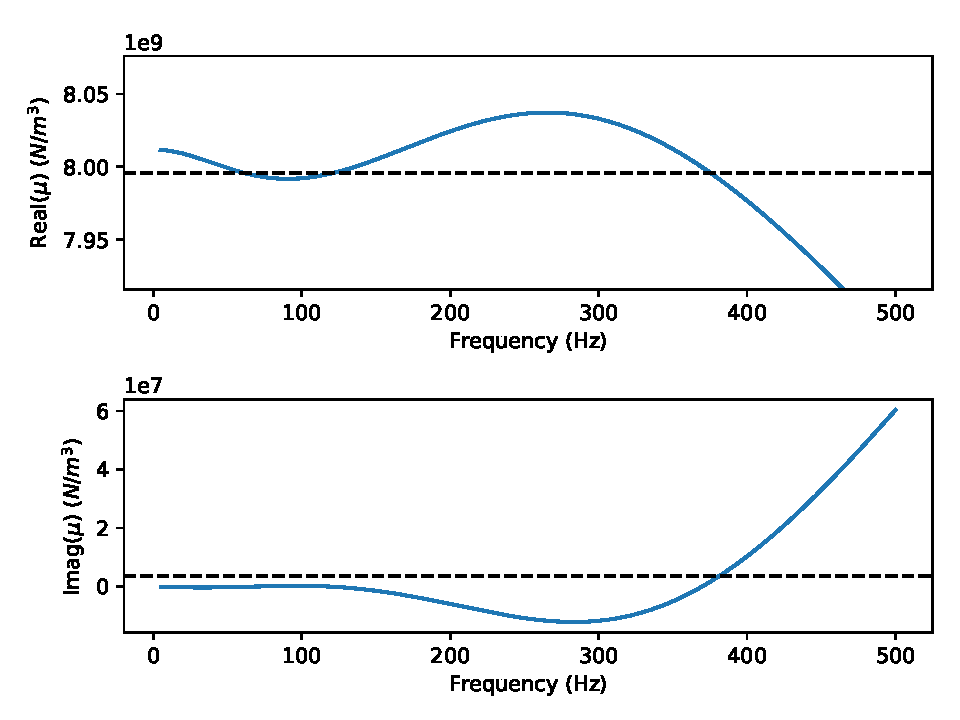
\includegraphics[width=\linewidth]{nlbeam/fnsi/knl0.pdf}
    \caption{}
  \end{subfigure}
  ~
  \begin{subfigure}[b]{0.45\textwidth}
    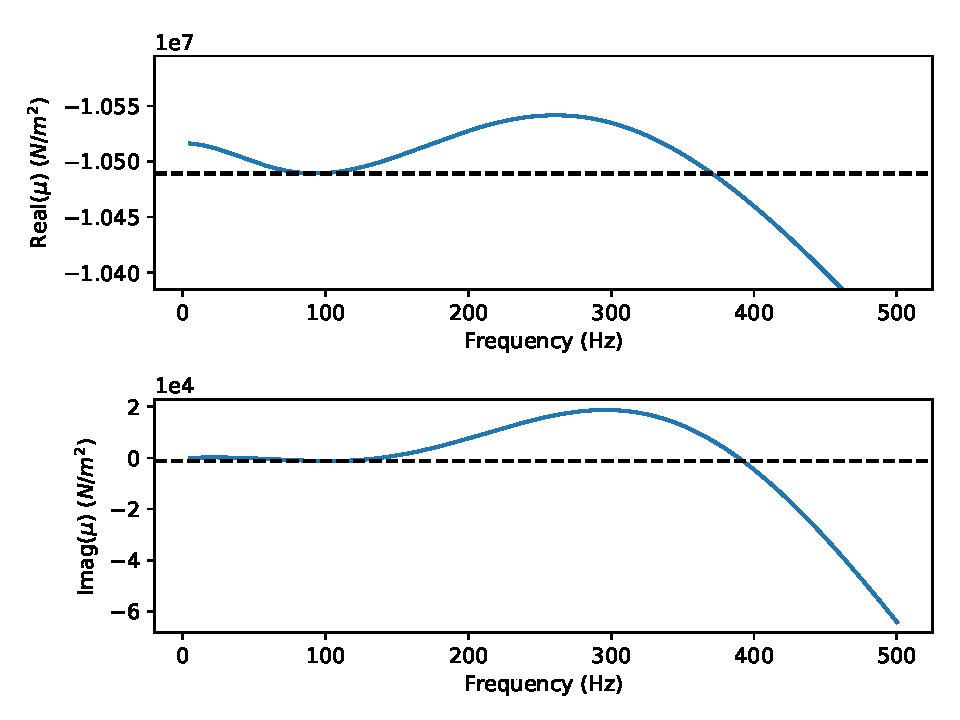
\includegraphics[width=\linewidth]{nlbeam/fnsi/knl1.pdf}
    \caption{}
  \end{subfigure}
  \caption{Real and imaginary part of estimated nonlinear coefficients $\mu_1$
    and $\mu_2$. The variation of Re($\mu$) is seen to be within a 1 interval.
    The imaginary part is about three orders of magnitude smaller. Both
    indicates a good quality of the estimation. The spectral averages of the
    real part and ratio $\text{log}_{10}\frac{\Re(\mu)}{\Im(\mu)}$ are:
    \textbf{(a)}: $\mu_1 = 8.0 \times 10^9 m/n^3$, ratio = 3.34;
    \textbf{(b)}: $\mu_2 = -1.05 \times 10^7 m/n^2$, ratio = 3.96.
  }
  \label{fig:nlbeam_knl}
\end{figure}


Finally fig. \ref{fig:nlbeam_frf} shows the FRF. Nonlinear distortion is seen
from the signal at high level excitation. The FRF(blue) from low level excitation and
identified by FNSI with basis functions(green) match.

\begin{figure}[!ht]
  \centering
  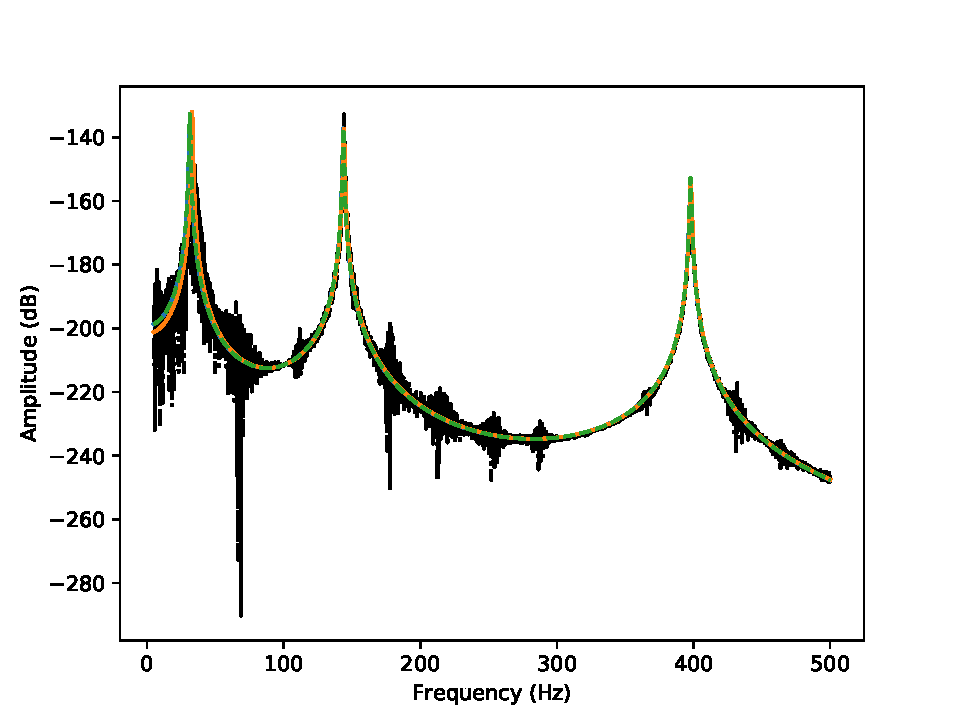
\includegraphics[width=0.6\textwidth]{nlbeam/fnsi/frf.pdf}
  \caption{FRF. Nonparametric(NP) is FRF directly from signal, parametric is
    identified FRF.
    \sampleline{}: NP from high level excitation;
    \textcolor{blue}{\sampleline{}}: NP from low level excitation.
    \textcolor{orange}{\sampleline{}}: Linear parametric from high level excitation.
    \textcolor{green}{\sampleline{dashed}}: nonlinear parametric from high level excitation.
}
  \label{fig:nlbeam_frf}
\end{figure}

\subsection{Design}

The test setup is modelled as shown in fig \ref{fig:nlbeam_fem}, using 14 and 3
two-dimensional Bernoulli-Euler beam elements for the main and thin beam
respectively. The connection between the two beams is modelled by an additional
linear rotational stiffness, as suggested in \autocite{lenaerts2003a}, resulting
in a model with 35 dofs.
% In traditional FEM, boundary conditions can be enforced
% in different ways; either modifying the stiffness matrix or the load vector.
% With the methods presented here, boundary conditions should always be enforced
% by modifying the stiffness matrix, i.e. for fixed dofs all rows and columns
% relating to these dofs are removed, which is why the system ends up having 35
% dofs.

\begin{figure}[!ht]
  \centering
  \def\svgwidth{10cm}
  \import{fig/nlbeam/}{beam_fem.pdf_tex}
  \caption{FE model of the COST beam.}
  \label{fig:nlbeam_fem}
\end{figure}

The geometric properties are also given in \autocite{lenaerts2003a} and listed
together with the mechanical properties in tables \ref{table:nlbeam_prop}.
\begin{center}
\begin{tabular}{l*{3}{c}}
  & Length(m) & Width (m) & Thickness (m) \\
  \hline
  Main beam & 0.7 & 0.014 & 0.014 \\
  Thin beam & 0.04 & 0.014 & 0.0005 \\
  \hline
\end{tabular}
\begin{tabular}{p{3.1cm}p{2cm}*{3}{c}}
  Young's modulus\newline (N/$m^2$) & Density\newline (kg/$m^3$) & $\mu_1$ (N/$m^3$) & $\mu_2$ (N/$m^2$) & Damping  \\
  \hline
  $2.05\times 10^{11}$ & 7800 & $8\cdot 10^{9}$ & $-1.05\cdot 10^{7}$ &  $\bm C = 3 \cdot 10^{-7} \bm K + 5\bm M$ \\
  \hline
\end{tabular}
\captionof{table}{Geometric and mechanical properties for the nonlinear beam}
\label{table:nlbeam_prop}
\end{center}


The damping is proportional damping and probably overestimated, giving a modal
damping ration of $1.27\%$ for the first linear mode which is high for a steel
beam. But large displacements tends to be higher damped, thus the damping is not
expected to be same for the linear and nonlinear case.

Figure \ref{fig:nlbeam_sweep} shows a comparison between a linear forward and
backward sine sweep with a sweep rate and the NFRC computed by HB. The response
is asymmetric due to the presence of the quadratic nonlinearity. The jump down
occurs because of the hardening behavior.

\begin{figure}[!ht]
  \centering
  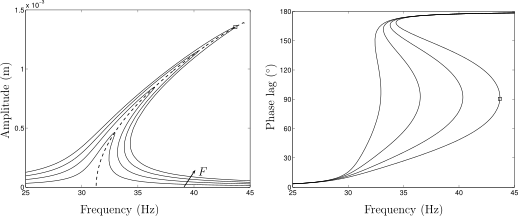
\includegraphics[width=0.7\textwidth]{nlbeam/hb/nfrc}
  \caption{Comparison between forward and backward sine sweep with HB. Sweep
    parameters: Amplitude: 3N, sweep rate: 10Hz/min. Stability is indicated for
    HB.}
  \label{fig:nlbeam_sweep}
\end{figure}

Figure \ref{fig:nlbeam_hb_components} shows the evolution of the harmonic
components along the curve. As expected from the asymmetry, there is strong
participation of the constant term, followed by the 2nd harmonic. Both due to
the squared nonlinearity.

\begin{figure}[!ht]
  \centering
  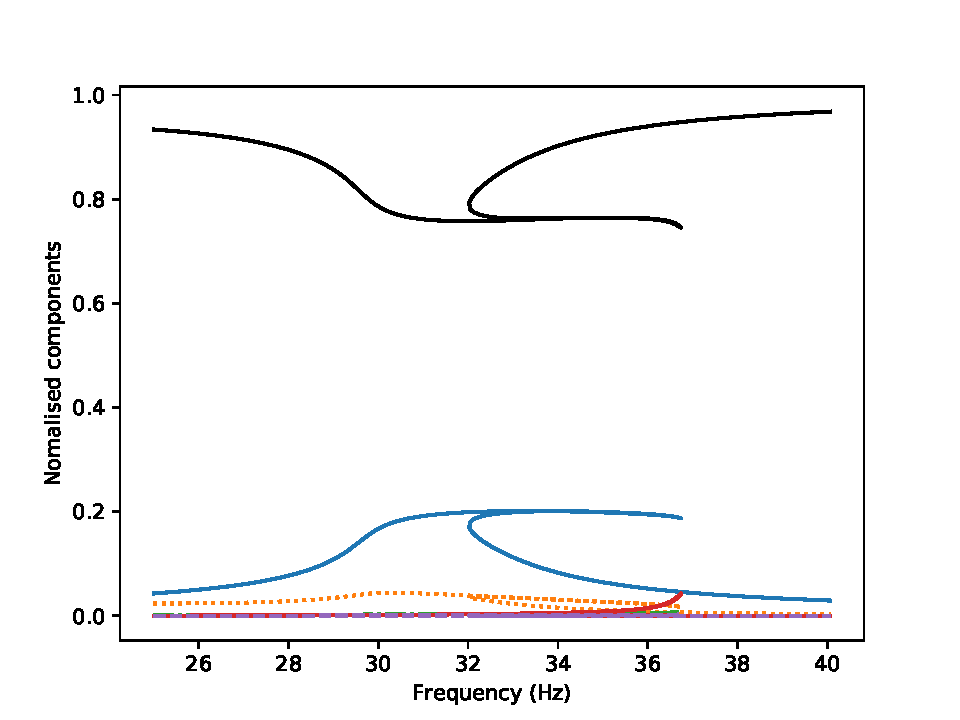
\includegraphics[height=6cm,width=0.7\textwidth]{nlbeam/hb/har}
  \caption{Evolution of HB components.
    \textcolor{blue}{\sampleline{}}: Constant;
    \sampleline{}: 1st;
    \textcolor{orange}{\sampleline{dotted}}: 2nd;
    \textcolor{green}{\sampleline{dash pattern=on .7em off .2em on .2em off .2em}}: 3th;
    \textcolor{red}{\sampleline{}}: 4th;
    \textcolor{purple}{\sampleline{dashed}}: 5th;
  }
  \label{fig:nlbeam_hb_components}
\end{figure}

% \textbf{NNM mangler - Plot fra 1.nnm er beskrevet. 2.nnm mangler at blive beregnet.}
% The NNMs of the underlying conservative system is shown in figure. The NNM
% frequency increases strongly with increasing energy, which is due to the
% hardening behavior of the cubic stiffness. The FEPs shows two branches emerging
% from the NNM backbone. These are called tongues and are said to reveal internal
% resonance. The tongue shows a 9:1 internal resonance between the first and third
% NNMs.

\FloatBarrier
\section{System with clearences}
\label{sec:syst-with-clear}

Ideen er at identificere clearence og parametre. Data genereres med en trilineær
model. Men da Newmark, mv. kræver at stivheden er differentiabel, bruges et
reguliseret udtryk. Det bliver forhåbent meget kortere end sidste eksempel. \textbf{Alt Mangler}.

A trilinear model for stiffness' $k_-, k, k_+$ and clearances $a_-, a_+$ is
given by, %\citet{renson2014_phd}
\begin{equation}
  \label{eq:fnl_piecewise}
  f_{nl}(x) =
  \begin{cases}
    \sign(x) \left( ka_+ + k_+(x-a_+) \right) & x \geq a_+ + \Delta_+ \\
    p_+(t(x)) & a_+ + \Delta_+ > x > a_+ - \Delta_+ \\
    kx & a_+ - \Delta_+ \geq -(a_- - \Delta_-) \\
    p_-(t(x)) & -(a_- + \Delta_-) > x > -(a_- + \Delta_-) \\
    \sign(x) \left( ka_- + k_-(x-a_-) \right) & x \leq -(a_- + \Delta_-) \\
  \end{cases}
\end{equation}
where $x$ is the relative distance between the two DOFs defining the nonlinear
connections. $2\Delta_\pm$ is the size of a regularization interval, used to
enforce continuity of the first derivative.

The Hermite polynomials $p_\pm$ are defined as
\begin{equation}
  \label{eq:fnl_herm_pol}
  p_\pm(t) = h_{00}(t)p_k + h_{10}(t)(x_{k+1}-x_k)m_k + h_{01}(t)p_{k+1} + h_{11}(t)(x_{k+1} - x_k)m_{k+1}
\end{equation}
where $p_k$ and $p_{k+1}$ are the values of the restoring force at points $x_k =
\sign(x)(a - \Delta)$ and $x_{k+1} = \sign(x)(a + \Delta)$, respectively. $m_k$
and $m_{k+1}$ are the values of the restoring force derivative at the same $x_k$
and $x_{k+1}$ points; they correspond to the stiffness coefficients k and
$k_\pm$, respectively. The local scaled abscissa and $h_{ij}$ functions are

\begin{equation}
  \label{eq:fnl_piecewise_coeff}
  \begin{aligned}
    t(x) &= \frac{x - x_k}{x_{k+1} - x_k}\\
    h_{00}(t) &=  2t^3 - 3t^2 + 1 \\
    h_{10}(t) &= t^3 - 2t^2 + t \\
    h_{01} &= -2t^3 + 3t^2 \\
    h_{11} &= t^3 - t^2 \\
  \end{aligned}
\end{equation}

Figure \ref{fig:fnl_piecewise} shows an example of a regulized nonlinear
restoring force.

\begin{figure}[!ht]
  \centering
  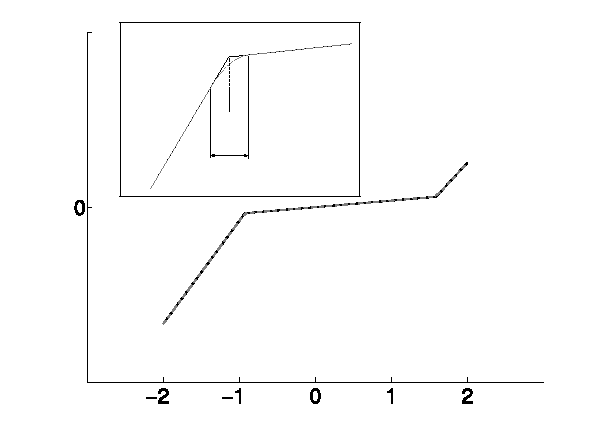
\includegraphics[width=0.7\textwidth]{appendix/piecewise_linear}
  \caption{Example of piecewise-linear restoring force. The insert image shows
    a closeup of the effect of the regularization $\Delta$.}
  \label{fig:fnl_piecewise}
\end{figure}



\FloatBarrier


%%% Local Variables:
%%% mode: latex
%%% TeX-master: "../report"
%%% End:

% \chapter{Discussion}
% \label{cha:discussion}
\chapter{Conclusion}
\label{cha:conclusion}

The focus of this report have been two-part. In the first part, methods for
vibration-based identification of localised nonlinearities have been explored and
validated. No assumption of the type of (localised) nonlinearity have been made, thus the
models works equally well for boundary, geometric, etc. types of nonlinearities.
Only stiffness have been treated; in theory the methods works just as well for
damping, but in practice damping is much harder due to the much smaller
magnitude and successful identification is still hard to obtain \autocite{noel2013a}.
Another subject that have been neglected, is identification using noisy
signals. The current FNSI implementation(in the vibration library) comes with
noise-weighting functions implemented as described by \autocite{noel2013a}(and
working accordingly to the description), but have not been tested en real noisy data.\\

In the second part, methods for investigating the behaviour of identified
nonlinear systems are treated. On the successful identification in part one, a
model is built and used for determine stability, bifurcations and internal
resonances. Where the methods in the first part requires some understanding and
knowledge about nonlinear system in order to obtain a good identification, the
methods here are easier to use and do not require as much knowledge (that said,
implementation wise they cannot be said to be easier).\\

One substantial lack in connecting the two parts, is the need to create a model
after identification is done. Current research are focused on eliminating this
step, and use the state space system identified by FNSI directly by the
numerical methods of the second part. Numerically this is
easy when both the FNSI and HB methods are implemented, but as shown in
\autocite{gourc2016a}, the FNSI method introduce spurious numerical
artefacts, and as long as these artefacts are present, the state space
formulation cannot be used directly. Preventing artefacts in the FNSI method
will be a big step forward in the seamless integration of the two methodologies.
Figure \ref{fig:fnsi_hb} shows the methodology.

\begin{figure}[!ht]
  \centering
  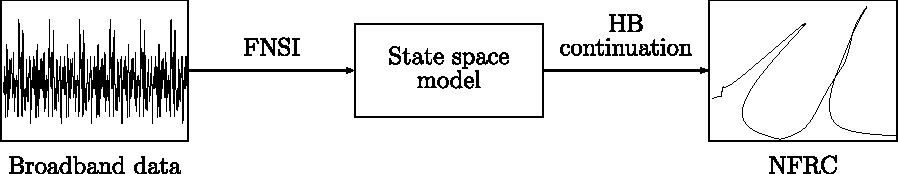
\includegraphics[width=0.7\linewidth]{discussion/fnsi_hb.pdf}
  \caption{FNSI-HB continuation procedure}
  \label{fig:fnsi_hb}
\end{figure}

This also concludes that focus have been on the methods, and efficient
implementation, and not application of them. The real limitations are not known
and using them on real life structures could be a complete project of it own.
For instance it have been assumed that a polynomial type of nonlinearity have a
integer order. This might not be case in real applications. FNSI can(or might) help
determine the polynomial order, but this have not been investigated.\\

Lacking in this thesis is the ability to track identified bifurcations.
This might be a potential feature in aiding designs: find the system parameters
where a bifurcation disappear. This could be exemplified as finding parameters
that prevents flutter. Bifurcation tracking is described in
\autocite{detroux2015a}. \\

As for the future of nonlinear system identification, progress have been made
within localised lumped nonlinearities - FNSI is just one of multiple methods - but
methods for distributed nonlinearities are still complicated and does not
convoy any physical interpretation due their flexible nature (ie. black box
models, where any combination of mathematical functions are mixed to model the
system.)\\



%%% Local Variables:
%%% mode: latex
%%% TeX-master: "../report"
%%% End:


% ------ Appendix ------
% \clearpage
% \setcounter{secnumdepth}{3}
% \addcontentsline{toc}{chapter}{Appendix}
\printbibliography[title=References]
% \appendix
% 
\chapter{Periodic solution}
\label{chap:per_sol}

\section{Shooting method}
\label{sec:shooting_appendix}

The state space formulated for the full eom \eqref{eq:per_eom} is

\begin{equation}
  \label{eq:app_state_space}
  \dot{\bm z}(t) = \bm L\bm z(t) - \bm g_{nl}(\bm z) + \bm g_{ext}(\omega,t)
\end{equation}
where

\begin{equation}
  \begin{aligned}
    \bm z =
    \begin{bmatrix}
      \bm x \\ \dot{\bm y}
    \end{bmatrix}, \quad
    \bm L =
    \begin{bmatrix}
      \bm 0 & \bm I_n \\
      -\bm M^{-1}\bm K & -\bm M^{-1} \bm C
    \end{bmatrix} \\
    \bm g_{nl} =
    \begin{bmatrix}
      \bm 0 \\ \bm M^{-1} \bm f_{nl}(\bm x, \dot{\bm x})
    \end{bmatrix}, \quad
    \bm g_{ext}
    \begin{bmatrix}
      \bm 0 \\ \bm M^{-1} \bm p_{ext}(\omega, t)
    \end{bmatrix}
  \end{aligned}
\end{equation}

Calculating the periodic motion for the full EOM, instead of the unforced and
undamped case as in section \ref{sec:shooting_method}, only requires changing
the evaluation of the state space to the formula above. The sensitivity analysis
in section \ref{sec:newmark_sens} is derived for the full EOM. Thus at max five
lines of code needs changing.

\section{HB}
\label{sec:hb_appendix}

The derivation of the equations of motion in frequency domain continues from
where it was left in section \ref{sec:harmonic_bal}.

The operators $\bm \nabla$ and $\bm \nabla^2$ used in expressing velocities and
accelerations are given as
\begin{equation}
  \label{eq:hb_nabla}
  \bm \nabla =
  \begin{bmatrix}
    \bm 0 &        &                &        & \\
          & \ddots &                &        & \\
          &        & \bm \nabla_k   &        & \\
          &        &                & \ddots & \\
          &        &                &        & \bm \nabla_{N_H}
  \end{bmatrix}, \quad
  \bm \nabla^2 =
  \begin{bmatrix}
    \bm 0 &        &                &        & \\
          & \ddots &                &        & \\
          &        & \bm \nabla^2_k &        & \\
          &        &                & \ddots & \\
          &        &                &        & \bm \nabla^2_{N_H}
  \end{bmatrix}
\end{equation}
with

\begin{equation}
  \label{eq:hb_nabla2}
  \bm \nabla_k =
  \begin{bmatrix}
    0       & -k\omega \\
    k\omega & 0
  \end{bmatrix}, \quad
  \bm \nabla^2_k =
  \begin{bmatrix}
    -(k\omega)^2 & 0 \\
    0            & -(k\omega)^2
  \end{bmatrix}
\end{equation}

Substitute eqs. \eqref{eq:hb_x_expansion}-\eqref{eq:hb_f_expansion} and
\eqref{eq:hb_vel}-\eqref{eq:hb_acc} into the EOM \eqref{eq:per_eom} to get

\begin{equation}
  \label{eq:hb_eom_subs}
  \bm M((Q(t)\bm\nabla^2) \otimes \mathbb{I}_n)\bm z  +
  \bm C((Q(t)\bm\nabla) \otimes \mathbb{I}_n)\bm z  +
  \bm K((Q(t) \otimes \mathbb{I}_n)\bm z  =
  (\bm Q(t)\otimes I_n) \bm b
\end{equation}

Using the mixed-product product of the Kronecker product $(\bm A \otimes \bm
B)=(\bm C \otimes \bm D) = (\bm A \bm C) \otimes (\bm B \bm D)$ gives


\begin{equation}
  \begin{aligned}
    \bm M((Q(t)\bm\nabla^2) \otimes \mathbb{I}_n) &=
    (1\otimes \bm M) ((\bm Q(t) \bm \nabla^2)\otimes I_n ) =
    (\bm Q(t)\bm \nabla^2)\otimes \bm M \\
    \bm C((Q(t)\bm\nabla) \otimes \mathbb{I}_n) &=
    (1\otimes \bm C) ((\bm Q(t) \bm \nabla)\otimes I_n ) =
    (\bm Q(t)\bm \nabla)\otimes \bm C \\
    \bm K(Q(t) \otimes \mathbb{I}_n) &=
    (1\otimes \bm K) (\bm Q(t) \otimes I_n ) =
    \bm Q(t)\bm \otimes \bm K
  \end{aligned}
\end{equation}

Substituting these into eq. \eqref{eq:hb_eom_subs} gives
\begin{equation}
  ((\bm Q(t)\bm \nabla^2) \otimes \bm M)\bm z +
  ((\bm Q(t)\bm \nabla) \otimes \bm C)\bm z +
  (\bm Q(t) \otimes \bm K)\bm z =
  (\bm Q(t) \otimes I_n) \bm b
  \label{eq:hb_eom_subs2}
\end{equation}

In order to remove the time dependency and to obtain an expression relating the
different Fourier coefficients, a Galerkin procedure projects eq.
\eqref{eq:hb_eom_subs2} on the orthogonal trigonometric basis $\bm Q(t)$

\begin{equation}
  \begin{aligned}
    \left( \left( \frac{2}{T}\int^T_0 \bm Q^T(t) \bm Q(t) \d t \bm \nabla^2
      \right) \otimes \bm M \right) \bm z +
    \left( \left( \frac{2}{T}\int^T_0 \bm Q^T(t) \bm Q(t) \d t \bm \nabla
      \right) \otimes \bm C \right) \bm z \\
    \left( \left( \frac{2}{T}\int^T_0 \bm Q^T(t) \bm Q(t) \d t
      \right) \otimes \bm K \right) \bm z =
    \left( \left( \frac{2}{T}\int^T_0 \bm Q^T(t) \bm Q(t) \d t
      \right) \otimes I_n \right) \bm b
  \end{aligned}
\end{equation}
where $T=2\pi / \omega$ is the period of the external force.

Using that
\begin{equation}
  \frac{2}{T}\int^T_0 \bm Q^T(t) \bm Q(t) \d t = I_{2N_H+1}
\end{equation}
the equations of motion expressed in frequency domain are

\begin{equation}
  %\label{eq:hb_feom}
  (\bm \nabla^2 \otimes \bm M)\bm z + (\bm \nabla \otimes \bm C)\bm z +
  (\mathbb{I}_{2N_H} \otimes \bm K)\bm z =
  (\mathbb{I}_{2N_H} \otimes \mathbb{I}_n )\bm b
\end{equation}
or in more compact form

\begin{equation}
  \label{eq:hb_feom_compact}
  \bm H(\bm z, \omega) = \bm A(\omega) \bm z - \bm b(\bm z) = \bm 0
\end{equation}
where $\bm A$ describes the linear dynamics

\begin{equation}
  \label{eq:hb_A}
  \begin{aligned}
    \bm A &= \bm \nabla^2 \otimes \bm M + \bm \nabla \otimes \bm C +
    \mathbb{I}_{2N_H} \otimes \bm K \\
    &=
    \begin{bmatrix}
      \bm K \\
      & \bm K - \omega^2 \bm M & -\omega \bm C \\
      & \omega \bm C & \bm K - \omega^2 \bm M \\
      & & & \ddots \\
      & & & & \bm K - (N_H \omega)^2 \bm M & -N_H \omega \bm C \\
      & & & & N_H \omega \bm C & \bm K - (N_H \omega)^2 \bm M
    \end{bmatrix}
  \end{aligned}
\end{equation}


\subsection{Stability}
\label{sec:hb_stab_appendix}

To find the stability of a periodic solution, a method known as \textit{Hills
  method} is used to estimate the Floquet exponents.

A periodic solution $\bm x(t)$ satisfying the eom eq. \eqref{eq:per_eom} is
perturbed by an exponential decay
\begin{equation}
  \label{eq:hb_pert}
  \bm p(t) = \bm x(t) + e^{\lambda t}\bm s(t)
\end{equation}
inserting this into the eom eq. \eqref{eq:per_eom},
\begin{equation}
  \bm M\ddot{\bm x} + \bm C\dot{\bm x} + \bm K\bm x +
  (\lambda^2 \bm M \bm s + \lambda(2\bm M \dot{\bm s}) +
  \bm M\ddot{\bm s} + \bm C\dot{\bm s} + \bm K \bm s ) e^{\lambda t} =
  \bm f(\bm p, \dot{\bm p}, \omega, t)
\end{equation}

Following the outline of section \ref{sec:harmonic_bal}, the solution and
perturbation are approximated by Fourier series truncated to $N_H$-th order,
i.e. $\bm x(t) = (\bm Q(t) \otimes I_n)\bm z$ and $\bm s(t) = (\bm Q(t) \otimes
I_n)\bm u$, where $\bm z$ and $\bm u$ contains the Fourier coefficients of $\bm
x$ and $\bm s$, respectively. Following section \ref{sec:hb_appendix}, a
Galerkin is used to obtain

\begin{equation}
  \bm A \bm z +
  (\bm \Delta_2\lambda^2 + \bm \Delta_1 \lambda + \bm A) e^{\lambda t} \bm u =
  \bm b(\bm z + e^{\lambda t} \bm u)
  \label{eq:hb_pert2}
\end{equation}
where $\bm \Delta$ are matrices describing the linear dynamics similar to $\bm
A$ in eq. \eqref{eq:hb_A} and $\lambda$ are Hills coefficients.

\begin{equation}
  \begin{aligned}
    \bm \Delta_1 &= \bm \nabla \otimes 2\bm M + \mathbb{I}_{2N_H+1} \otimes \bm C \\
    &=
    \begin{bmatrix}
      \bm C \\
      & \bm C & -\omega \bm M \\
      & 2\omega \bm M & \bm C \\
      & & & \ddots \\
      & & & & \bm C & -2N_H \omega \bm M \\
      & & & & 2N_H \omega \bm M & \bm C
    \end{bmatrix} \\
    \bm \Delta_2 &= \mathbb{I}_{2N_H+1} \otimes \bm M
  \end{aligned}
\end{equation}

The right-hand side of eq. \eqref{eq:hb_pert2} is evaluated through a Taylor series expansion around
the solution $\bm z$
\begin{equation}
  \bm b(\bm z+e^{\lambda t} \bm u) = \bm b(\bm z) + \frac{\p \bm b}{\p \bm z}\big|_z (e^{\lambda t}\bm u)
\end{equation}

Since $\bm A \bm z - \bm b(\bm z) = \bm 0$ by definition and given that
\begin{equation}
  \bm A - \frac{\p \bm b}{\p \bm z}\big|_z = \bm h_{\bm z}
\end{equation}
eq. \eqref{eq:hb_pert2} is rewritten into the quadratic eigenvalue problem

\begin{equation}
  \left( \bm \Delta_2 \bm \lambda^2 + \bm \Delta_1 \bm \lambda + \bm H_{\bm z}  \right)
  e^{\lambda t} \bm u = \bm 0
\end{equation}


\subsection{NNM}
\label{sec:hb_nnm_appendix}

Following the method above, NNMs can be computed using HB in the following way:

\begin{equation}
  \bm h_{ham} (\bm z, \omega) = (\bm \nabla^2 \otimes \bm M) \bm z +
  (I_{2N_H+1} \otimes \bm K) \bm z + \bm b_{nl} = \bm 0
\end{equation}
where $\bm b_{nl}$ is the vector of the Fourier coefficients of the nonlinear
forces, defined as
\begin{equation}
  \bm f_{nl}(\bm x) = (\bm Q(t)\otimes I_n) \bm b_{nl}
\end{equation}

The phase condition for frequency-domain methods are often to set a Fourier
coefficient of a DOF to zero. Doing this, the equation for a NNM motion is
\begin{equation}
  \label{eq:hb_nnm}
  \bm h_{NNM} =
  \begin{bmatrix}
    \bm h_{ham}(\bm z, \omega) \\ z_i
  \end{bmatrix}
  = \bm 0
\end{equation}
where $z_i$ is a component of $\bm z$.

%%% Local Variables:
%%% mode: latex
%%% TeX-master: "../../report"
%%% End:

% 
\chapter{Continuation}
\label{chap:cont_appendix}

\section{Harmonic balance}
\label{sec:hb_appendix}

Figure \ref{fig:hb_frf_appendix} shows the influence of the included number of
harmonics $N_H$, The time discretisation $N$ and the optimal number of
iterations $I_{opt}$. Fig. \ref{fig:hb_frf_a_appendix} shows superharmonic
resonances at low frequencies are not captured for $N_H=3$ and $N_H=1$. This is
expected as they possesses multiple frequency content, but shows that care
should be taken when the number of harmonics is selected. Especially for more
complicated and rich vibrations that this simple example.
For systems with few DOFs, it is not a problem to include a high number of
harmonics - remember that system matrices $\bm A$ in the HB method, eq
\eqref{eq:hb_A}, is of size $(2N_H + 1)n \times (2N_H + 1)n$ and the sparse
Fourier operator $\bm \Gamma$ of size $nH \times(2N_H+1)n$ where $n$ is number
of DOFs. But for large systems it will become a problem. To solve this,
\citet{GROLET2012a} present a way to automatically adopt the number of harmonics
for each DOF.

Fig. \ref{fig:hb_frf_b_appendix} shows that the solution is inaccurate around
the peak for lower $N$. This is due to aliasing effects.{\textbf -- Det slap du
  nu lidt for nemt om ved --}

Fig. \ref{fig:hb_frf_c_appendix} shows that the peak is ``cut short'' or
truncated for higher values of $I_{opt}$. Setting a high value of $I_{opt}$
allows for taking larger steps, since more Newton iterations are allowed to
correct the guess. Thus resolution is decreased. Of course one can use a
\texttt{max\_step} parameter to prevent too large steps.

\begin{figure}[ht!]
  \centering
  \begin{subfigure}[b]{0.7\textwidth}
    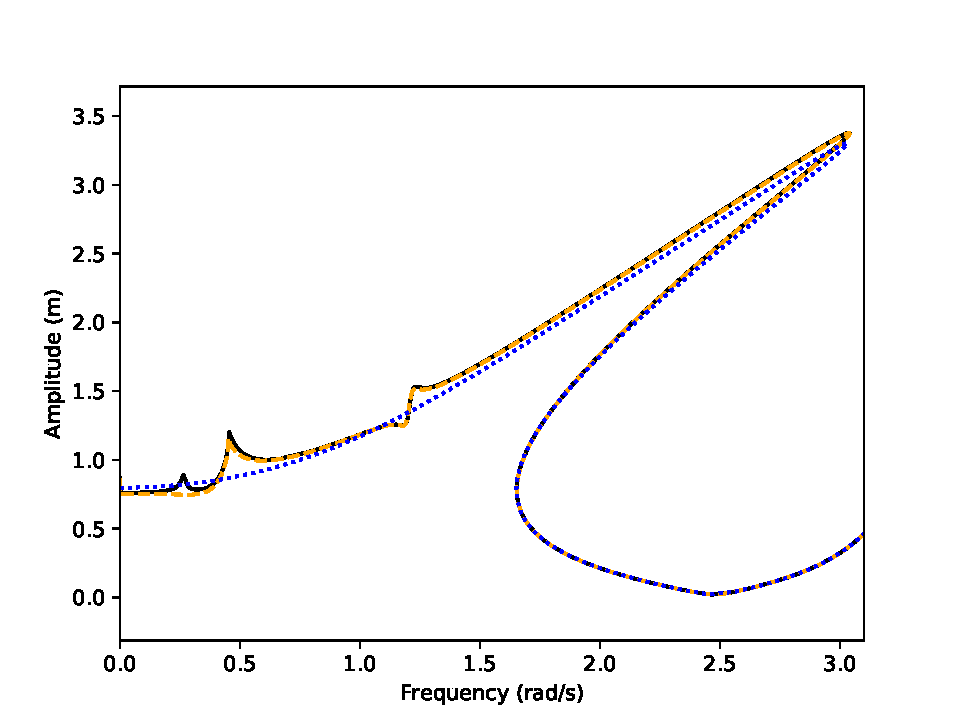
\includegraphics[width=\linewidth, height=8cm]{2dof_duffing/hb_nh.tikz}
    \caption{}
    \label{fig:hb_frf_a_appendix}
  \end{subfigure}\\
  \begin{subfigure}[b]{0.45\textwidth}
    \includegraphics[width=\linewidth, height=5cm]{2dof_duffing/hb_N.tikz}
    \caption{}
    \label{fig:hb_frf_b_appendix}
  \end{subfigure}~
  \begin{subfigure}[b]{0.45\textwidth}
    \includegraphics[width=\linewidth, height=5cm]{2dof_duffing/hb_ipopt.tikz}
    \caption{}
    \label{fig:hb_frf_c_appendix}
  \end{subfigure}
  \caption{NRFC of the coupled duffing system for $x_1$ with $f=2$N. Influence
    of HB and continuation parameters, compared to $N_H=5, N=512, I_{opt}=3$ (\sampleline{}).
    Stability is not shown.
    \textbf{(a)}
    (\sampleline{dashed}) $N_H=3$;
    (\sampleline{dotted}) $N_H=1$;
    \textbf{(b)}
    (\sampleline{dashed}) $N=128$;
    (\sampleline{dotted}) $N=64$;
    \textbf{(c)}
    (\sampleline{dashed}) $I_{opt}=5$;}
  \label{fig:hb_frf_appendix}
\end{figure}




%%% Local Variables:
%%% mode: latex
%%% TeX-master: "../../report"
%%% End:

% 
\chapter{Signals}
\label{chap:signals}


%%% Local Variables:
%%% mode: latex
%%% TeX-master: "../../report"
%%% End:

% 
\chapter{Newmark integration}
\label{chap:newmark-integration}

Newmarks time integration is used for solving the initial value problem defined by
the EOM,

\begin{align}
  \label{eq:nm_eom}
    \begin{aligned}
  &\bm M \ddot{\bm x}(t) + \bm C_v \dot{\bm x}(t) + \bm K \bm x(t) +
    \bm f_{nl} \left( \bm x(t), \dot{ \bm x}(t) \right) = \bm p(t) \\
  &\qquad \bm z_0 =
  \begin{bmatrix}
    \bm x(0) \\
    \dot{\bm x}(0)
  \end{bmatrix}
  =
  \begin{bmatrix}
    \bm x_0 \\
    \dot{\bm x}_0
  \end{bmatrix}
\end{aligned}
\end{align}
where $\bm z_0$ are the initial conditions. $\bm z$ is the state vector.

The associated sensitivity problem, ie. how sensitive the current motion is to
the initial conditions, is given by
\begin{equation}
  \label{eq:nm_sens}
  \begin{aligned}
  &\bm M  \frac{\p \ddot{ \bm x}(t)}{\p \bm z_0}  +
  \bm C_v \frac{\p \dot{\bm x}(t)}{\p \bm z_0}  +
  \bm K \frac{\p \bm x(t)}{\p \bm z_0}  +
    \frac{\p \bm f_{nl}}{\p \bm x} \bigg|_{\bm x(t)}
    \frac{\p \bm x(t)}{\p \bm z_0} +
    \frac{\p \bm f_{nl}}{\p \dot{\bm x}} \bigg|_{\dot {\bm x}(t)}
    \frac{\p \dot{ \bm x}(t)}{\p \bm z_0} =
  \bm 0 \\
  &\qquad
  \begin{bmatrix}
    \frac{\p \bm x(0)}{\p \bm z_0} \\
    \frac{\p \dot{\bm x}(0)}{\p \bm z_0}
  \end{bmatrix}
  = \bm I
    \end{aligned}
\end{equation}
where $\frac{\p \ddot{ \bm x}(t)}{\p \bm z_0}$ is implied to mean
$\frac{\d^2}{\d t^2} \left[\frac{\p \bm x(t)}{\p \bm z_0} \right]$

\section{Solving EOM}
\label{sec:nm_solve_eom}


The solution of the EOM is done by an implicit nonlinear Newmark scheme.
Description of the method can be found in \textcite{krenk2009non}.

Here follows a more throughout derivation. The algorithm itself, for fixed time
step, is shown in pseudo-code in Algorithm \ref{algo:nonlin_newmark}.


The residual of the EOM eq. \eqref{eq:nm_eom} is

\begin{equation}
  \label{eq:nm_res}
  \bm r (\bm x) = \bm M \ddot{\bm x}(t) + \bm C \dot{\bm x}(t) + \bm K \bm x(t) +
    \bm f_{nl} \left( \bm x(t), \dot{ \bm x}(t) \right) - \bm p(t) = 0
\end{equation}

From time $t$ to $t+h$, a Taylor series expansion of the velocity and
displacement with respect to $h$ gives

\begin{equation}
  \label{eq:nm_taylor}
  \begin{aligned}
    \dot {\bm x}_{t+h} &= \dot{\bm x}_t + (1-\gamma)h \ddot{\bm x}_t + \gamma h \ddot{\bm x}_{t+h} \\
    {\bm x}_{t+h} &= \bm x_t + \dot{\bm x}_t + (\frac{1}{2}-\beta)h^2 \ddot{\bm x}_t + \beta h^2 \ddot{\bm x}_{t+h}
  \end{aligned}
\end{equation}
where $\gamma$ and $\beta$ are weighting constants. Often $\gamma =\frac{1}{2},
\beta = \frac{1}{4}$ is chosen, which is the Average Acceleration method. This
gives a scheme that is unconditionally stable and converges as
$\mathcal{O}(h^2)$

This can be rewritten as

\begin{align}
  \label{eq:nm_taylor2}
  &\begin{aligned}
    \dot {\bm x}_{t+h} &= \dot{\bm x}^*_{t+h} + \gamma h \ddot{\bm x}_{t+h} \\
    \bm x_{t+h} &= \bm x^*_{t+h} + \beta h^2 \ddot{\bm x}_{t+h}
  \end{aligned} \\
  &\begin{aligned}
    \dot {\bm x}^*_{t+h} &= \dot{\bm x}_t + (1-\gamma)h \ddot{\bm x}_t  \\
    {\bm x}^*_{t+h} &= \bm x_t + \dot{\bm x}_t + (\frac{1}{2}-\beta)h^2 \ddot{\bm x}_t
  \end{aligned}
\end{align}
where $(^*)$ denotes prediction. The prediction depends on the previous time
step $t$ and implies the prediction $\ddot{\bm x}^*_{t+h} = 0$.

Rewriting eq. \eqref{eq:nm_taylor2} again
\begin{equation}
  \label{eq:nm_scheme}
  \begin{aligned}
    &\ddot{\bm x}_{t+h} = \frac{1}{\beta h^2} (\bm x_{t+h} - \bm x^*_{t+h}) \\
    &\dot{\bm x}_{t+h} = \dot{\bm x}^*_{t+h} \frac{\gamma}{\beta h} (\bm x_{t+h} - \bm x^*_{t+h})
  \end{aligned}
\end{equation}

Substituting this into the residual eq. \eqref{eq:nm_res}, the equation is only
expressed in terms of $\bm x_{t+h}$. Due to the nonlinear stiffness and
dissipation, the residual equation have to be solved iteratively by Newton-Raphson
iterations.


\begin{equation}
  \label{eq:nm_nr}
  \bm r(\bm x^k_{t+h}) + \bm S(\bm x^k_{t+h}) \bm \Delta \bm x = 0
\end{equation}

The iteration matrix $\bm S$, also called the tangent stiffness, is given by

\begin{equation}
  \label{eq:nm_tangent}
  \bm S(\bm x^k_{t+h}) = \left[ \frac{\d \bm r}{\d \bm x} \right]_{\bm x^k_{t+h}} =
  \frac{1}{\beta h^2} \bm M + \frac{\gamma}{\beta h} \bm C + \bm K +
  \frac{\p \bm f_{nl}}{\p \bm x} +
  \frac{\gamma}{\beta h} \frac{\p \bm f_{nl}}{\p \dot{ \bm x}}
\end{equation}

Thus the correction is found by solving eq. \eqref{eq:nm_nr}

\begin{equation}
  \label{eq:nm_nr2}
  \Delta \bm x^k_{t+h} = - \bm S(\bm x^k_{t+h})^{-1} \bm r(\bm x^k_{t+h})
\end{equation}
and updating the state variables

\begin{equation}
  \begin{aligned}
    &\bm x^{k+1}_{t+h} = \bm x^k_{t+h} + \Delta \bm x^k_{t+h} \\
    &\dot{\bm x}^{k+1}_{t+h} = \dot{\bm x}^k_{t+h} +
    \frac{\gamma}{\beta h} \Delta \bm x^k_{t+h} \\
    &\ddot{\bm x}^{k+1}_{t+h} = \ddot{\bm x}^k_{t+h} +
    \frac{1}{\beta h^2} \Delta \bm x^k_{t+h} \\
  \end{aligned}
\end{equation}

The Newton iterations are carried out until some norm of residual value is below
a given tolerance. \textcite{cook2007concepts} have different examples of norms that
can be used.


\section{Sensitivity Equations}
\label{sec:newmark_sens}


At the end of each time step, the sensitivity matrix $\left[ \frac{\p \bm x}{\p
    \bm z_0} \right]$ is found by solving eq. \eqref{eq:nm_sens}.
Using Newmarks scheme given by eq. \eqref{eq:nm_scheme}, at time step $t+h$ one have

\begin{align}
\label{eq:nm_sens_xdd}
  &\left[ \frac{\p \ddot{\bm x}}{\p \bm z_0} \right]_{t+h} =
    \frac{1}{\beta h^2} \left(
    \left[ \frac{\p \bm x}{\p \bm z_0} \right]_{t+h} -
    \left[ \frac{\p \bm x}{\p \bm z_0} \right]^*_{t+h}
    \right) \\
\label{eq:nm_sens_xd}
  &\left[ \frac{\p \dot{\bm x}}{\p \bm z_0} \right]_{t+h} =
    \left[ \frac{\p \dot{\bm x}}{\p \bm z_0} \right]^*_{t+h} +
    \frac{\gamma}{\beta h^2} \left(
    \left[ \frac{\p \bm x}{\p \bm z_0} \right]_{t+h} -
    \left[ \frac{\p \bm x}{\p \bm z_0} \right]^*_{t+h}
    \right)
\end{align}
the predictions are given as (* denote prediction)

\begin{align}
  \label{eq:nm_sens_predict}
  &\left[ \frac{\p \dot{\bm x}}{\p \bm z_0} \right]^*_{t+h} =
    \left[ \frac{\p \dot{\bm x}}{\p \bm z_0} \right]_{t} +
    (1-\gamma)h \left[ \frac{\p \ddot {\bm x}}{\p \bm z_0} \right]_{t} \\
  &\left[ \frac{\p \bm x}{\p \bm z_0} \right]^*_{t+h} =
    \left[ \frac{\p \bm x}{\p \bm z_0} \right]^*_{t}
    h \left[ \frac{\p \dot {\bm x}}{\p \bm z_0} \right]_{t} +
    h^2(\frac{1}{2} - \beta) \left[ \frac{\p \ddot{\bm x}}{\p \bm z_0} \right]_{t}
\end{align}


By rearranging and substitution eqs. \eqref{eq:nm_sens_xdd} and
\eqref{eq:nm_sens_xd} into the linear sensitivity eq. \eqref{eq:nm_sens}, the
sensitivity acceleration matrix at time $t+h$ is found as

\begin{align}
  &\frac{1}{\beta h^2}
  \left[
    \frac{1}{\beta h^2} \bm M +
    \frac{\gamma}{\beta h} \bm C +
    \bm K +
    \frac{\p \bm f_{nl}}{\p \bm x} +
    \frac{\gamma}{\beta h} \frac{\p \bm f_{nl}}{\p \dot{\bm x}}
  \right]
    \left[ \frac{\p \ddot{\bm x}}{\p \bm z_0} \right]_{t+h} = \nonumber \\
 & -
  \left(\bm K + \frac{\bm \p f_{nl}}{\p \bm x} \right)
  \left[ \frac{\p \bm x}{\p \bm z_0} \right]^*_{t+h}
  -
  \left(\bm C + \frac{\bm \p f_{nl}}{\p \dot {\bm x}} \right)
  \left[ \frac{\p \dot{\bm x}}{\p \bm z_0} \right]^*_{t+h}
  \label{eq:nm_sens_sol}
\end{align}
from where the sensitivity matrix is found by \eqref{eq:nm_sens_xdd}.


Thus by marching in time, the current motion and its sensitivity with respect to
initial conditions are found.

\section{Algorithm}
\label{sec:newmark_algo}


\begin{algorithm}
  % \setstretch{1.30} % For article class
  \setSpacing{1.30}
  Initial conditions, $\bm x_0, \dot{\bm x}_0$. \linebreak
  $A_1 = (1 - \gamma) h, \quad
  B_1 = (\frac{1}{2} - \beta) h^2, \quad
  A_2 = \frac{1}{\beta h^2}, \quad
  B_2 = \frac{\gamma}{\beta h}$  \linebreak
  $\bm S_{lin} = \bm K + \frac{\gamma}{\beta h} \bm C + \frac{\beta}{h^2} \bm M$  \linebreak
  $\ddot{\bm x}_0 = \bm M^{-1}(\bm p_0 - \bm C \dot{\bm x}_0 - \bm K \bm x_0 -
  \bm f_{nl}\left( \bm u_0,\dot{\bm u}_0 \right))$  \linebreak
  \If{sensitivity}{
  \nonl$\bm V = [\bm I,\bm 0; \bm 0, \bm 0], \dot{\bm V} = [\bm 0,\bm
  0;\bm 0,\bm I]$ \\
  \nonl$\ddot{\bm V} = - \bm M^{-1} \left((\bm C + \bm f_{nl,\dot{\bm x}}) \dot{\bm
      V} + (\bm K  + \bm f_{nl,\bm x}) {\bm V} \right)$
}
\For{$n \gets 0$ \KwTo $nt$}{

  Prediction step (time integration): \linebreak
  $\dot{\bm x}_{n+1} = \dot{\bm x}_{n} + A_1 \ddot{\bm x}_n$ \linebreak
  $\bm x_{n+1} = {\bm x}_{n} + h \dot{\bm x}_n + B_1 \ddot{\bm x}_n$ \linebreak
  $\ddot{\bm x}_{n+1} = 0$

  Residual calculation: \linebreak
  $\bm r = \bm M \ddot{\bm x}_{n+1} + \bm f_{nl} + \bm f_{l} -  \bm p_{n+1}$

  \While{norm($\bm r$) > tol}{
    \nonl NR iteration (increment correction) \linebreak
    $\bm S_{eff} = \bm f_{nl, \bm x} + B_2\bm f_{nl, \dot{ \bm x}} + \bm S_{lin}$  \linebreak
    $\Delta \bm x = - \bm S_{eff}^{-1} \bm r$ \linebreak
    $ \ddot{\bm x}_{n+1} += A_2 \Delta \bm x$ \linebreak
    $ \dot{\bm x}_{n+1} += B_2 \Delta \bm x$ \linebreak
    $\bm x_{n+1} += \Delta \bm x$

    $\bm r = \bm M \ddot{\bm x}_{n+1} + \bm f_{nl} + \bm f_{l} -  \bm p_{n+1}$
  }
  \If{sensitivity}{
    prediction \linebreak
    $\bm V = \bm V + h\dot{\bm V} + B_1 \ddot{\bm V}$\linebreak
    $\dot{\bm V} = \dot{\bm V} + A_1 \ddot{\bm V}$\linebreak
    correction \linebreak
    $\bm S = \bm S_{lin} + \bm f_{nl, \bm x} + B_2 \bm f_{nl,
      \dot{\bm x}}$\linebreak
    $\bm S = \beta h^2 \bm S$\linebreak
    $\ddot{\bm V} = -\bm S^{-1}\left[
      (\bm C + \bm f_{nl, \dot{\bm x}} )\dot{\bm V} +
      (\bm K + \bm f_{nl, \bm x} ) \bm V  \right]$ \linebreak
    $\bm V = \bm V + \beta h^2 \ddot{\bm V}$ \linebreak
    $\dot{\bm V} = \dot{\bm V} + \gamma h \ddot{\bm V}$\linebreak
  }
}
  \caption{Nonlinear Newmark algorithm}
  \label{algo:nonlin_newmark}
\end{algorithm}

\subsection{Summary}

The Newmark-beta method used for implicit time integration was developed in
1959. Today it is one of the most widely used solvers for dynamics systems, and
for most problems it performs reasonable well. For problems with very stiff and
very flexible parts, i.e. where eigenvalues are very separated, it performs
poorly due to lack of high frequency numerical damping. Interested readers are
referred to \cite{bathe2012a}, which also suggest one alternative (it should be
noted that what Bathe calls the Newmark trapezoidal rule is mostly known as the
Newmark average acceleration method).


%%% Local Variables:
%%% mode: latex
%%% TeX-master: "../../report"
%%% End:

% 
\chapter{Easter egg}
\label{chap:easter_egg}

Congratulations. You got through and there is no more. This note is not about
vibrations, but some few things on how you(as a student) do linear algebra
fast(er) without any effort.

Whenever you find eigenvalues, do SVD decompistion or solve linear systems, you
use linear algebra. In the end of the seventies a specification for numerical
linear algebra was made called Basic Linear Algebra Subprograms(BLAS), together
with a reference implementation written i \texttt{Fortran 77}. Later came an
extension to BLAS, Linear Algebra Package(LAPACK), also written in \texttt{f77}.
These specifications are the de-facto standard today. So when you call
\texttt{eigs} or \texttt{\textbackslash} in matlab, matlab calls LAPACK and BLAS
compatible routines under the hood.

Now when we run a program, there are many small things that impact performance
we do not think or care about. These things the software takes care of. For
instance if we multiply two matrices, then the program decides how the CPU
should access the memory where the arrays are stored. It decides which rows and
columns of the arrays should be in the fast accessible caches, when memory is
moved, what the block size should be, etc. The optimal settings for these things
differs from architecture to architecture(ie. is it a Pentium, Intel Core, AMD,
etc. cpu).

Thus it makes a big difference if the BLAS implementation is optimised for your
computer. The old reference implementation is not written with these
optimisation in mind, especially because said architectures did not exist back
then. Still it is the standard implementation that follows with many program.

Today (and for the past five years at least) the best implementation of BLAS and
ATLAS references are the intel MKL and Openblas libraries. MLK is free for
students but not open source. Openblas is completely free and open source -
choose that one. To show the difference, figure ... shows the computation time
for matrix multiplication for python compiled with Openblas and the standard
(old reference). The speed difference is remarkable and is the same for all
other linear algebra operations.

Default BLAS \& LAPACK
Dotted two 4096x4096 matrices in 64.22 s.
Dotted two vectors of length 524288 in 0.80 ms.
SVD of a 2048x1024 matrix in 10.31 s.
Cholesky decomposition of a 2048x2048 matrix in 6.74 s.
Eigendecomposition of a 2048x2048 matrix in 53.77 s.

OpenBLAS
Dotted two 4096x4096 matrices in 3.97 s.
Dotted two vectors of length 524288 in 0.74 ms.
SVD of a 2048x1024 matrix in 1.96 s.
Cholesky decomposition of a 2048x2048 matrix in 0.46 s.
Eigendecomposition of a 2048x2048 matrix in 32.95 s.

As an extra example, I wrote a matrix multiplication function in \texttt{C}.
General matrix multiplication is simple, just three loop through rows and
columns and multiply elements (while this kind of looping of course is a sin in
matlab, that is the way you should do it manually in compiled languages like C
and fortran. In fact explicit loops in C are faster than vectorizing in matlab).
The program was 12 times slower than the reference BLAS and ATLAS. The point is,
there is no way you can do linear algebra faster than ``production''
implementations of BLAS and the used version of BLAS matters for speed.

As a closing note: If you want to go really fast, you go parallel using
clusters. To help you with that, use \texttt{PETSc} which does message parsing,
preconditioning and includes a variety of iterative solvers. But \textit{that}
takes a bit of effort.

Ps.
I gave the impression that matlab comes with a slow version of BLAS. That is not
the case. Matlab(closed source and expensive) comes with Intel MKL. But why not
try python, Julia or some of the other open source languages, that are well
suited for scientific calculation and plotting. It is now, when still in
university you have the time.

PPs.
The general matrix multiplication algorithm/implementation scales at
$\mathbb{O}(n^3)$(asymtotic complexity). The fastest matrix multiplication
algorithm changes with size matrix size, since even if they scaly better, the
constant in front might make them unpractical for smaller matrices. A general
matrix algorithm that performs good is the Strassen algorithm, scaling at
$\mathbb{O}(n^{2.81})$.

PPPs.
Performance BLAS libraries are not written in fortran anymore. They are written
in a combination of assembly and C-code.


%%% Local Variables:
%%% mode: latex
%%% TeX-master: "../../report"
%%% End:


\end{document}

%%% Local Variables:
%%% mode: latex
%%% TeX-master: t
%%% End:
